% \setcounter{section}{5}
% \setcounter{dang}{0}
% \section{Thực hành tính xác xuất theo định nghĩa cổ điển}
% \subsection{Tóm tắt lí thuyết}
% \subsubsection{Phép thử}
% \begin{dn}
% 	Phép thử ngẫu nhiên là phép thử mà ta không đoán trước được kết quả của phép thử đó mặc dù biết tập tất cả các kết quả của phép thử đó.
% \end{dn}
% \subsubsection{Biến cố}
% %%\setcounter{vd}{0}
% \begin{dn}
% Biến cố là một tập con của không gian mẫu.
% \end{dn}
% \begin{note}
% \begin{listEX}
% \item Biến cố $A$ liên quan đến phép thử $T$ là biến cố mà việc xảy ra hay không xảy ra của $A$ tùy thuộc vào kết quả của $T$.
% \item Mỗi kết quả của phép thử $T$ làm cho $A$ xảy ra gọi là một kết quả thuận lợi của $A$.
% \item Biến cố $A$ có ngoài cách cho bằng mô tả, có thể cho $A$ dưới dạng liệt kê tất cả các kết quả thuận lợi của $A$.
% \end{listEX}
% \end{note}
% \subsubsection{Xác suất}
% %%\setcounter{vd}{0}
% \begin{dn}
% Xét phép thử $T$ có không gian mẫu $\Omega$ là một tập hữu hạn kết quả đồng khả năng. Biến cố $A$ liên quan đến phép thử, $A\subset \Omega$. Xác suất của biến cố $A$ là 
% $$\mathrm{P}\left(A\right)=\dfrac{n(A)}{n(\Omega)}.$$
% \end{dn}
% \begin{note}
% \begin{listEX}
% \item Với mọi biến cố $A$ của phép thử có không gian mẫu là $\Omega$. Ta luôn có 
% $0\le \mathrm{P}\left(A\right)\le 1$.
% \item $\mathrm{P}\left(A\right)=1-\mathrm{P}\left(\overline{A}\right)$, trong đó $\overline{A}$ là biến cố đối của biến cố $A$.
% \item Với $A,B$ là hai biến cố ta có $n(A\cup B)=n(A)+n(B)-n(A\cap B)$.
% \end{listEX}
% \end{note}
% \subsection{Các dạng toán}
\begin{dang}{Các bài toán về người và vật áp dụng trực tiếp định nghĩa cổ diển}
\end{dang}
\viduminhhoa	
\begin{vd}
	Gieo một con súc sắc cân đối và đồng chất. Tính xác suất để xuất hiện mặt hai chấm.
	\loigiai{
		\begin{itemize}
			\item Số trường hợp của không gian mẫu là $n(\Omega)=6$.
			\item Gọi $A$ là biến cố xuất hiện mặt hai chấm. Số trường hợp thuận lợi của $A$ là $n(A)=1$.
			\item Xác suất xuất hiện mặt hai chấm là $\mathrm{P}(A)=\dfrac{n(A)}{n(\Omega)}=\dfrac{1}{6}$.
		\end{itemize}
	}
\end{vd}
\begin{vd}
	Gieo một con súc sắc cân đối và đồng chất. Tính xác suất để xuất hiện mặt có số chấm lớn hơn $3$.
	\loigiai{
		\begin{itemize}
			\item Số trường hợp của không gian mẫu là $n(\Omega)=6$.
			\item Gọi $A$ là biến cố xuất hiện mặt có số chấm lớn hơn $3$, suy ra $A=\{4;5;6\}$. Số trường hợp thuận lợi của $A$ là $n(A)=3$.
			\item Xác suất xuất hiện mặt có số chấm lớn hơn $3$ là $\mathrm{P}(A)=\dfrac{n(A)}{n(\Omega)}=\dfrac{3}{6}=\dfrac{1}{2}$.
		\end{itemize}
	}
\end{vd}
\begin{vd}
	Gieo hai con súc sắc cân đối đồng chất khác nhau. Tính xác suất để tổng số chấm trên hai mặt xuất hiện của hai con súc sắc bằng $8$.
	\loigiai{
		\begin{itemize}
			\item Không gian mẫu là $ \Omega=\{(1;1),\,(1;2),\,(2;1),\,(1;3),\,(3;1),\,\ldots,\,(5;6),\,(6;6)\} $.\\
			Số phần tử của không gian mẫu là $ n(\Omega) = 6\cdot 6=36 $.
			\item Gọi $A$ là biến cố \lq\lq Tổng số chấm trên hai mặt xuất hiện của hai con súc sắc bằng $8$\rq\rq.\\
			Tập hợp mô tả biến cố $A$ là $ A=\{(2;6),\,(6;3),\,(3;5),\,(5;3),\,(4;4)\} $.
			\item Xác suất cần tìm là $ \mathrm{P}=\dfrac{n(A)}{n(\Omega)}=\dfrac{5}{36}$.
		\end{itemize}
	}
\end{vd}
\begin{vd}
	Có $15$ quả cầu được đánh số từ $1$ đến $15$. Chọn ngẫu nhiên một quả cầu, tính xác suất chọn được một quả cầu mang số lẻ.
	\loigiai{
		\begin{itemize}
			\item Chọn $1$ quả cầu trong $15$ quả cầu có $15$ cách chọn.
			\item Gọi $A$ là biến cố chọn được quả cầu mang số lẻ, suy ra $n(A)=8$.
			\item Xác suất chọn được quả cầu mang số lẻ là $\mathrm{P}(A)=\dfrac{8}{15}$.
		\end{itemize}
	}
\end{vd}
\begin{vd}
	Một lớp học có $22$ nam và $18$ nữ. Giáo viên cần chọn $2$ học sinh để đi trực sao đỏ, tính xác suất để chọn được $1$ nam và $1$ nữ.
	\loigiai{
		\begin{itemize}
			\item Chọn $2$ học sinh trong $40$ học sinh có $\mathrm{C}^2_{40}=780$ cách.
			\item Gọi $A$ là biến cố chọn được $1$ nam và $1$ nữ. Suy ra $n(A)=22\cdot 18=396$ cách.
			\item $\mathrm{P}(A)=\dfrac{396}{780}=\dfrac{33}{65}$.
		\end{itemize}
	}
\end{vd}
\begin{vd}
	Lớp $11B$ có $25$ đoàn viên trong đó có $10$ nam và $15$ nữ. Chọn ngẫu nhiên $5$ đoàn viên trong lớp để tham dự hội trại ngày 26 tháng 3. Tính xác suất để $5$ đoàn viên được chọn có $2$ nam và $3$ nữ.
	\loigiai{
		\begin{itemize}
			\item Chọn ngẫu nhiên $5$ đoàn viên có $\mathrm{C}_{25}^5$ cách.
			\item Chọn $5$ đoàn viên sao cho có $2$ nam và $3$ nữ có $\mathrm{C}_{10}^2\cdot \mathrm{C}_{15}^3$ cách.
			\item Xác suất cần tìm là $\dfrac{195}{506}$.
		\end{itemize}
	}
\end{vd}
\begin{vd}
	Một tổ có $5$ nữ và $4$ nam. Giáo viên cần chọn $4$ người làm vệ sinh lớp. Tính xác suất để $4$ người được chọn có đúng một bạn nam.
	\loigiai{
		\begin{itemize}
			\item Số cách chọn $4$ học sinh bất kỳ trong $9$ học sinh là $n(\Omega)=\mathrm{C}_9^4=126$.
			\item Gọi $A$ là biến cố chọn được đúng một nam trong $4$ người được chọn,\\ suy ra $n(A)=\mathrm{C}_4^1\cdot \mathrm{C}_5^3=40$.
			\item Vậy xác suất chọn được đúng một nam trong $4$ người được chọn là $\mathrm{P}(A)=\dfrac{40}{126}=\dfrac{20}{63}$.
		\end{itemize}
	}
\end{vd}
\begin{vd}
	Từ một hộp có $7$ quả cầu màu đỏ và $5$ quả cầu màu xanh, lấy ngẫu nhiên đồng thời $3$ quả cầu. Tính xác suất để được $3$ quả cầu màu xanh.
	\loigiai{
		\begin{itemize}
			\item Số phần tử của không gian mẫu là $n(\Omega)=\mathrm{C}_{12}^3=220$.
			\item Gọi biến cố $A\colon$ \lq\lq Lấy ra được $3$ quả màu xanh\rq\rq.\\
			Số kết quả thuận lợi cho biến cố $A$ là $n(A)=\mathrm{C}_5^3=10$.
			\item Xác suất của biến cố $A$ là $\mathrm{P}(A)=\dfrac{10}{220}=\dfrac{1}{22}.$
		\end{itemize}
	}
\end{vd}
\begin{vd}
	Có $4$ quả cầu trắng, $5$ quả cầu đỏ, $6$ quả cầu xanh. Chọn ngẫu nhiên $3$ quả cầu. Tính xác suất để chọn được $3$ quả cầu cùng màu.
	\loigiai
	{
		\begin{itemize}
			\item Số phần tử của không gian mẫu là $n(\Omega)=\mathrm{C}_{15}^3=455$.
			\item Gọi $A$ là biến cố \lq\lq chọn được $3$ quả cầu cùng màu\rq\rq.\\
			Số phần tử của biến cố $A$ là $n(A)=\mathrm{C}_4^3+\mathrm{C}_5^3+\mathrm{C}_6^3=34$.
			\item Vậy xác suất của biến cố $A$ là $\mathrm{P}(A)=\dfrac{n(A)}{n(\Omega)}=\dfrac{34}{455}$.
		\end{itemize}
	}
\end{vd}

\begin{vd}
	Một hộp có $4$ viên bi trắng, $5$ viên bi đỏ và $6$ viên bi vàng (các viên bi cùng màu thì giống nhau). Lấy ngẫu nhiên đồng thời từ hộp ra $4$ viên bi. Xác suất để lấy được $4$ viên bi có đủ $3$ màu.
	\loigiai{
		Lấy ngẫu nhiên 4 viên bi từ hộp chứa 15 viên bi có $n(\Omega)=\mathrm{C}_{15}^4=1365$ cách.\\
		Gọi $A$ là biến cố lấy được 4 viên bi có đủ cả 3 màu.
		\begin{itemize}
			\item Lấy được 2 bi trắng, 1 đỏ, 1 vàng có $\mathrm{C}_4^2\cdot\mathrm{C}_5^1\cdot\mathrm{C}_6^1=180$ cách.
			\item Lấy được 1 bi trắng, 2 đỏ, 1 vàng có $\mathrm{C}_4^1\cdot\mathrm{C}_5^2\cdot\mathrm{C}_6^1=240$ cách.
			\item Lấy được 1 bi trắng, 1 đỏ, 2 vàng có $\mathrm{C}_4^1\cdot\mathrm{C}_5^1\cdot\mathrm{C}_6^2=300$ cách.
		\end{itemize}
		Vậy $n(A)=180+240+300=720$ cách. \\
		Xác suất của biến cố $A$ là $\mathrm{P}(A)=\dfrac{n(A)}{n(\Omega)}=\dfrac{720}{1365}=\dfrac{48}{91}$.
	}
\end{vd}
\baitaptl
\setcounter{bt}{0}
\begin{bt}
	Chọn ngẫu nhiên một số từ tập hợp $X$, với $X=\{0, 1, 2, 3, 4, 5, 6, 7\}$. Tính xác suất để số được chọn là số chẵn.
	\loigiai{
		\begin{itemize}
			\item Chọn ngẫu nhiên một số từ $X$, ta có số phần tử của không gian mẫu là $n(\Omega)=8$.
			\item Gọi $A$ là biến cố \lq\lq chọn được số chẵn\rq\rq. Ta có số phần tử của $A$ là $n(A)=4$.
			\item Xác suất cần tìm $\mathrm{P}(A)=\dfrac{n(A)}{n(\Omega)}=\dfrac{4}{8}=\dfrac{1}{2}$.
		\end{itemize}
	}
\end{bt}
\begin{bt}
	Gieo một đồng tiền cân đối và đồng chất $4$ lần. Tính xác suất để cả $4$ lần đều xuất hiện mặt sấp.
	\loigiai{
		\begin{itemize}
			\item Số phần tử của không gian mẫu là $n\left(\Omega\right)=2^4=16.$
			\item Số phần tử của biến cố $A$ để cả $4$ lần đều xuất hiện mặt sấp là $n\left(A\right)=1$.
			\item Xác suất của biến cố $A$ là $\mathrm{P}(A)=\dfrac{n(A)}{n\left(\Omega\right)}=\dfrac{1}{16}$.
		\end{itemize}
	}
\end{bt}
\begin{bt}
	Có $7$ tấm bìa được đánh số từ $1$ đến $7$, mỗi tấm bìa ghi một số. Rút ngẫu nhiên ba tấm bìa. Tính xác suất của biến cố \lq\lq Tổng các số trên ba tấm bìa bằng $12$\rq\rq.
	\loigiai{
		\begin{itemize}
			\item Rút ngẫu nhiên 3 tấm bìa từ 7 tấm bìa là $n(\Omega)=\mathrm{C}_7^3=35$ cách chọn.
			\item Gọi $A$ là biến cố \lq\lq Tổng các số trên ba tấm bìa bằng 12\rq\rq.\\
			Khi đó $A=\{(1;4;7), (1;5;6), (2;4;6), (2;3;7), (3;4;5)\}$. Ta có $n(A)=5$ cách chọn.
			\item Xác suất của biến cố $A$ là $\mathrm{P}(A)=\dfrac{n(A)}{n(\Omega)}=\dfrac{5}{35}=\dfrac{1}{7}$.
		\end{itemize}
	}
\end{bt}
\begin{bt}
	Trong một nhóm gồm $8$ học sinh trong đó có hai bạn Đức và Thọ. Chọn ngẫu nhiên $3$ học sinh từ nhóm học sinh trên. Tính xác suất để $3$ học  được chọn ra phải có Đức và Thọ.
	\loigiai{
		\begin{itemize}
			\item Số phần tử của không gian mẫu $n (\Omega)=\mathrm{C}_8^3=56$.
			\item Số cách chọn $3$ học sinh có Đức và Thọ là  $n(A)=\mathrm{C}_6^1=6$.
			\item Xác suất $\mathrm{P}(A)=\dfrac{6}{56}=\dfrac{3}{28}$.
		\end{itemize}
	}
\end{bt}
\begin{bt}
	Một thùng sữa có $12$ hộp sữa khác nhau, trong đó có $7$ hộp sữa cam và $5$ hộp sữa dâu. Lấy ngẫu nhiên ra $2$ hộp sữa trong thùng trên. Tính xác suất để hai hộp được lấy có cả hai loại.
	\loigiai{
		\begin{itemize}
			\item Chọn $2$ hộp sữa bất kì trong $12$ hộp sữa có $\mathrm{C}^2_{12} = 66$ cách.
			\item Số cách chọn để lấy được hai hộp sữa có cả hai loại là $7\cdot 5 = 35$.
			\item Xác suất cần tìm là $\dfrac{35}{66}.$
		\end{itemize}
	}
\end{bt}

\begin{bt}
	Một người chọn ngẫu nhiên $2$ chiếc giày từ $5$ đôi giày cỡ khác nhau. Tính xác suất để $2$ chiếc giày được chọn tạo thành một đôi.
	\loigiai{
		\begin{itemize}
			\item Chọn ngẫu nhiên $2$ chiếc giày từ $10$ chiếc giày nên mỗi lần chọn ta có kết quả là một tổ hợp chập $2$ của $10$ phần tử.\\
			Vậy số phần tử của không gian mẫu là $\mathrm{C}_{10}^2=45$.
			\item Gọi $A$ là biến cố \lq\lq Hai chiếc được chọn tạo thành một đôi\rq\rq.\\
			Ta có $n(A)=5$.
			\item Vậy $\mathrm{P}(A)=\dfrac{5}{45}=\dfrac{1}{9}$.
		\end{itemize}
	}
\end{bt}
\begin{bt}
	Một hộp đựng $4$ viên bi trắng, $5$ viên bi đen và $6$ viên bi đỏ. Lấy ngẫu nhiên từ hộp đó $3$ viên bi. Tính xác suất để ba viên bi được lấy ra có đủ ba màu.
	\loigiai{
		\begin{itemize}
			\item Số phần tử của không gian mẫu $n(\Omega)=\mathrm{C}_{15}^3=455$.
			\item Gọi $A$ là biến cố \lq\lq ba viên bi lấy ra có đủ ba màu\rq\rq.\\
			Khi đó $n(A)=\mathrm{C}_4^1\cdot \mathrm{C}_5^1\cdot\mathrm{C}_6^1=120$.
			\item Vậy xác suất của biến cố $A$ là $\mathrm{P}(A)=\dfrac{n(A)}{n\left(\Omega\right)}=\dfrac{120}{455}=\dfrac{24}{91}$.
		\end{itemize}
	}
\end{bt}
\begin{bt}
	Một hộp bi có $6$ viên bi xanh và $4$ viên bi đỏ. Lấy ngẫu nhiên $3$ viên bi từ hộp bi đó. Tính xác suất để $3$ viên bi lấy được là $3$ viên bi cùng màu.
	\loigiai{
		Số cách lấy ngẫu nhiên $3$ viên bi từ hộp là $n(\Omega)=\mathrm{C}_{10}^3$.\\
		Gọi $A$ là biến cố \lq\lq Lấy được $3$ viên bi cùng màu\rq\rq. Khi đó $n(A)=\mathrm{C}_{6}^3+\mathrm{C}_{4}^3$.\\
		Xác suất của biến cố $A$ là $\mathrm{P}(A)=\dfrac{n(A)}{n(\Omega)}=\dfrac{\mathrm{C}_{6}^3+\mathrm{C}_{4}^3}{\mathrm{C}_{10}^3}=\dfrac{1}{5}$.
	}
\end{bt}
\begin{bt}
	Cho hai đường thẳng song song $a$ và $b$. Trên đường thẳng $a$ lấy $6$ điểm phân biệt, trên đường thẳng $b$ lấy $5$ điểm phân biệt. Chọn ngẫu nhiên $3$ điểm trong các điểm đã cho trên hai đường thẳng $a$ và $b$. Tính xác suất $P$ để $3$ điểm được chọn tạo thành một tam giác.
	\loigiai{
		\begin{itemize}
			\item Chọn ngẫu nhiên ba điểm từ các điểm đã cho, số cách chọn là $n(\Omega) = \mathrm{C}_{11}^3 = 165$.
			\item Để ba điểm được chọn tạo thành tam giác ta cần chọn hai điểm thuộc $a$ và một điểm thuộc $b$ hoặc ngược lại. Do đó số cách chọn ba điểm tạo thành tam giác là $n(A) = \mathrm{C}_{5}^2 \cdot \mathrm{C}_{6}^1 + \mathrm{C}_{5}^1 \cdot \mathrm{C}_{6}^2 = 135$.
			\item Do đó $P = \dfrac{135}{165} = \dfrac{9}{11}.$
		\end{itemize}
	}
\end{bt}
\begin{bt}
	Có hai hộp đựng cầu, mỗi hộp đựng $30$ quả cầu được đánh số từ $1$ đến $30$ và các quả cầu trong hai hộp khác màu. Chọn ngẫu nhiên từ mỗi hộp đó một quả cầu. Tính xác suất để trong hai quả cầu được chọn có tích hai số ghi trên hai quả cầu đó là một số chia hết cho $6$.
	\loigiai{
		Ta đặt $A=\{1;2;\ldots;30\}$, $B$ là tập các số tự nhiên từ $1$ đến $30$ và chia hết cho $6$, $C$ là tập các số tự nhiên từ $1$ đến $30$ chia hết cho $2$ nhưng không chia hết cho $6$, $D$ là tập các số tự nhiên từ $1$ đến $30$ chia hết cho $3$ nhưng không chia hết cho $6$. Khi đó ta có
		$B=\{6;12;18;24;30\}$, $C=\{2;4;8;10;14;16;20;22;26;28\}$ và $D=\{3;9;15;21;27\}$.\\
		Vì các quả cầu là khác màu và khác số nên không gian mẫu của phép thử là
		\[\Omega = \{(i;j)|i;j \in A\} \Rightarrow n\left(\Omega\right) =30^2 =900.\]
		Để chọn được hai quả cầu có tích hai số ghi trên hai quả cầu đó là một số chia hết cho $6$ có các khả năng sau
		\begin{itemize}
			\item Trường hợp chọn được cả hai quả cầu có số chia hết cho $6$ có $5\cdot 5=25$ khả năng.
			\item Trường hợp chọn được đúng một quả cầu có số chia hết cho $6$ và một quả cầu có số không chia hết cho $6$ có $2\cdot 5\cdot 25 = 250$ khả năng.
			\item Trường hợp chọn được cả hai quả cầu có số đều không chia hết cho $6$. Khi đó ta chọn một quả cầu có số thuộc tập $C$ và một quả cầu có số thuộc tập $D$. Trường hợp này có $2\cdot 10\cdot 5 = 100$ khả năng.
		\end{itemize}
		Số thuận lợi của việc chọn được hai quả cầu có tích hai số ghi trên hai quả cầu đó là một số chia hết cho $6$ là $n(A)=375$.\\
		Vậy xác suất tìm được là $\mathrm{P}(A)=\dfrac{n(A)}{n\left(\Omega\right)} = \dfrac{375}{900} = \dfrac{5}{12}$.}
\end{bt}
\begin{dang}{Phương pháp tính xác suất dựa vào biến cố đối}
\end{dang}
\viduminhhoa
\setcounter{vd}{0}
\begin{vd}
	Gieo ngẫu nhiên một con xúc sắc cân đối và đồng chất hai lần. Tính xác suất để mặt sáu chấm xuất hiện ít nhất một lần.
	\loigiai
	{
		\begin{itemize}
			\item Số các kết quả đồng khả năng là $n(\Omega)=6\cdot 6=36$.
			\item Gọi $A$ là biến cố \lq\lq Mặt sáu chấm xuất hiện ít nhất một lần\rq\rq.\\
			Suy ra $\overline{A}$ là biến cố \lq\lq Không xuất hiện mặt sáu chấm\rq\rq .\\
			Ta có $n(\overline{A})=5\cdot 5=25$, $\mathrm{P}(\overline{A})=\dfrac{25}{36}$.
			\item Vậy $\mathrm{P}(A)=1-\mathrm{P}(\overline{A})=1-\dfrac{25}{36}=\dfrac{11}{36}$.
		\end{itemize}
	}
\end{vd}	
\begin{vd}
	Trên giá sách có $4$ quyển sách toán, $3$ quyển sách lý, $2$ quyển sách hóa. Lấy ngẫu nhiên $3$ quyển sách. Tính xác suất để trong ba quyển sách lấy ra có ít nhất một quyển là toán.
	\loigiai{
		\begin{itemize}
			\item Số cách chọn $3$ quyển sách là $\mathrm{C}_9^3=84$.
			\item Goi $A$ là biến cố \lq\lq chọn được $3$ quyển sách và ít nhất một quyển là toán\rq\rq.\\
			Suy ra $\overline{A}$ là biến cố \lq\lq chọn được $3$ quyển sách và không có quyển toán\rq\rq, $n(\overline{A})=\mathrm{C}_5^3=10$.
			\item Xác suất cần tìm là $\mathrm{P}(A)=1-\mathrm{P}(\overline{A})=1-\dfrac{10}{84}=\dfrac{37}{42}$.
		\end{itemize}
	}
\end{vd}
\begin{vd}
	Một tổ có $10$ học sinh trong đó có $4$ nam và $6$ nữ. Thầy chủ nhiệm cần chọn một nhóm gồm $3$ học sinh làm trực nhật. Tính xác suất để trong ba người được chọn phải có học sinh nữ.
	\loigiai{
		Số phần tử của không gian mẫu là $n(\Omega)=\mathrm{C}_{10}^3$.\\
		Gọi $A$ là biến cố chọn ba người học sinh đi trực nhật phải có học sinh nữ.\\
		Suy ra $\overline{A}$ là biến cố chọn ba người học sinh đi trực nhật không có học sinh nữ.\\
		Số cách chọn của biến cố $\overline{A}$ là $\mathrm{C}_4^3$.\\
		Xác suất của $\overline{A}$ là $\mathrm{P}(\overline{A})=\dfrac{\mathrm{C}_4^3}{\mathrm{C}_{10}^3}=\dfrac{1}{30}$.\\
		Vậy xác suất để trong ba người được chọn phải có học sinh nữ là $\mathrm{P}(A)=1-\mathrm{P}(\overline{A})=\dfrac{29}{30}$.
	}
\end{vd}
\begin{vd}
	Một chi đoàn có $40$ người, trong đó có $4$ cặp vợ chồng. Ban chấp hành cần chọn ra $3$ người để bầu vào các chức vụ: Bí thư, Phó bí thư, Thư kí. Tính xác suất để 3 người được chọn không có cặp vợ chồng nào.
	\loigiai
	{
		\begin{itemize}
			\item Số phần tử của không gian mẫu là $\mathrm{A}_{40}^3=52980$.
			\item Gọi $A$ là biến cố $3$ người được chọn không có cặp vợ chồng nào.\\
			Biến cố đối $\overline{A}$ là $3$ người được chọn có $1$ cặp vợ chồng.
			\item Ta tính số phần tử của biến cố $\overline{A}$.\\
			Chọn $1$ cặp vợ chồng trong $4$ cặp có $4$ cách.\\
			Chọn $1$ người trong $38$ người còn lại có $38$ cách.\\
			Từ $3$ người vừa chọn bầu vào $3$ chức vụ có $3!$ cách.\\
			$n(\overline{A})=4\cdot 38 \cdot 3!=912$.\\
			$n(A)=52980-n(\overline{A})=52980-912=58368$.
			\item $\mathrm{P}(A)=\dfrac{58368}{52980}=\dfrac{64}{65}$.
		\end{itemize}
	}
\end{vd}
\begin{vd}
	Một lô hàng gồm $30$ sản phẩm tốt và $10$ sản phẩm xấu. Lấy ngẫu nhiên $3$ sản phẩm. Tính xác suất để $3$ sản phẩm lấy ra có ít nhất một sản phẩm tốt.
	\loigiai
	{
		\begin{itemize}
			\item Số phần tử của không gian mẫu là $n\left(\Omega\right)=\mathrm{C}_{40}^3=9880$.
			\item Gọi $A$ là biến cố \lq\lq $3$ sản phẩm lấy ra có ít nhất một sản phẩm tốt\rq\rq.\\
			Suy ra $\overline{A}$ là biến cố \lq\lq $3$ sản phẩm lấy ra không có sản phẩm tốt\rq\rq,  $n\left(\overline{A}\right)=\mathrm{C}_{10}^3=120$.
			\item Xác suất của biến cố $A$ là $\mathrm{P}(A)=1-\mathrm{P}(\overline{A})=1-\dfrac{120}{9880}=\dfrac{9760}{9880}=\dfrac{244}{247}$.
		\end{itemize}
	}
\end{vd}
\begin{vd}
	Xét các số tự nhiên gồm $5$ chữ số khác nhau được lập từ các số $1, 3, 5, 7, 9$. Tính xác suất để tìm được một số không bắt đầu bởi $135$.
	\loigiai{
		\begin{itemize}
			\item Số phần tử không gian mẫu là $n(\Omega)=5!=120$.
			\item Gọi $A$ là biến cố \lq\lq số tìm được không bắt đầu bởi $135$\rq\rq.\\
			biến cố đối $\overline{A}$ là biến cố \lq\lq số tìm được bắt đầu bởi $135$\rq\rq.\\
			Ta tính số các kết quả thuận lợi cho biến cố đối.\\
			Buộc các số $135$ lại thì ta còn $3$ phần tử. Số các số tạo thành thỏa mãn số $135$ đứng đầu là $n(\overline{A})=1\cdot 2\cdot 1= 2$.\\
			Suy ra $n(A)=120-2=118$.
			\item Xác suất của biến cố $A$ là $\mathrm{P}(A)=\dfrac{118}{120}=\dfrac{59}{60}$.
		\end{itemize}
	}
\end{vd}
\begin{vd}
	Có $5$ cây viết đen, $6$ cây viết đỏ, $9$ cây viết xanh. Chọn ngẫu nhiên $3$ cây viết. Tính xác suất để chọn được ít nhất $1$ cây viết đen.
	\loigiai
	{
		\begin{itemize}
			\item Số phần tử không gian mẫu là $n(\Omega)=\mathrm{C}_{20}^3=1140$.
			\item Gọi $A$ là biến cố \lq\lq chọn được ít nhất $1$ cây viết đen\rq\rq.\\
			Suy ra $\overline{A}$ là biến cố \lq\lq chọn được $0$ cây viết đen\rq\rq, $n(\overline{A})=\mathrm{C}_{15}^3=455$.
			\item Xác suất của biến cố $A$ là $\mathrm{P}(A)=1-\mathrm{P}(\overline{A})=1-\dfrac{455}{1140}=\dfrac{137}{228}$.
		\end{itemize}
	}
\end{vd}
\begin{vd}
	Một hộp quà đựng $16$ dây buộc tóc cùng chất liệu, cùng kiểu dáng nhưng khác nhau về màu sắc. Cụ thể trong hộp có $8$ dây xanh, $5$ dây đỏ, và $3$ dây vàng. Bạn An được chọn ngẫu nhiên 6 dây từ hộp quà để làm phần thưởng cho mình. Tính xác suất để trong $6$ dây bạn An chọn có ít nhất $1$ dây vàng và không quá $4$ dây đỏ.
	\loigiai
	{
		\begin{itemize}
			\item Chọn ngẫu nhiên 6 dây từ 16 dây thì số cách chọn là $n(\Omega)=\mathrm{C}_{16}^6=8008$.
			\item Gọi $A$ là biến cố \lq\lq $6$ dây bạn An chọn có ít nhất $1$ dây vàng và không quá $4$ dây đỏ\rq\rq.\\
			Gọi $\overline{A}$ là biến cố đối của $A$, khi đó các trường hợp thuận lợi cho $\overline{A}$ là\\
			\textbf{TH1.} Không có dây nào vàng, số cách lấy là $\mathrm{C}_{13}^6$.\\
			\textbf{TH2.} Có $1$ dây vàng và $5$ dây đỏ, số cách lấy là $\mathrm{C}_{3}^1 \cdot \mathrm{C}_{5}^5$.\\
			Suy ra $n(\overline{A})=\mathrm{C}_{13}^6 + \mathrm{C}_{3}^1 \cdot \mathrm{C}_{5}^5=1719$.
			\item $n(A)=n(\Omega)-n(\overline{A})=8008-1719=6289$.
			\item $\mathrm{P}(A)=\dfrac{6289}{8008}$.
		\end{itemize}
	}
\end{vd}
\begin{vd}
	Gọi $S$ là tập các số tự nhiên có hai chữ số. Từ tập $S$ chọn ra $3$ số bất kì. Tính xác suất để trong $3$ số được chọn có ít nhất một số chia hết cho $5$.
	\loigiai{
		\begin{itemize}
			\item Tập $S= \{10; 11; 12; ..; 99\}$ có $90$ số.\\
			Các số chia hết cho 5 mà thuộc tập $S$ là $\{10; 15; 20; ..95\}$ có $18$ số.\\
			Có $90-18= 72$ số không chia hết cho $5$ từ tập $S$.\\
			Số phần tử của không gian mẫu là $\mathrm{C}_{90}^3$.
			\item Gọi $A$ là biến cố \lq\lq trong $3$ số được chọn có ít nhất một số chia hết cho $5$\rq\rq.\\
			Biến cố đối $\overline{A}$ là \lq\lq trong $3$ số được chọn không có số nào chia hết cho $5$\rq\rq.\\
			Số kết quả thuận lợi cho $\overline{A}$ là $n(\overline{A})=\mathrm{C}_{72}^3$.\\
			\item Suy ra $\mathrm{P}(\overline{A})=\dfrac{\mathrm{C}_{72}^3}{\mathrm{C}_{90}^3}=\dfrac{497}{979}$.\\
			$\mathrm{P}(A)=1-\mathrm{P}(\overline{A})=\dfrac{482}{979}$.
		\end{itemize}
	}
\end{vd}
\begin{vd}
	Đội thanh niên tình nguyện của nhà trường có $20$ học sinh, trong đó có $5$ học sinh khối $12$, $8$ học sinh khối $11$ và $7$ học sinh khối $10$. Chọn ngẫu nhiên $4$ học sinh trong đội thanh  niên tình nguyện của nhà trường đi làm nhiệm vụ. Tính xác suất để $4$ học sinh được chọn có đủ cả ba khối $10,11$ và $12$.
	\loigiai
	{
		Số cách chọn ngẫu nhiên $4$ học sinh trong đội thanh  niên tình nguyện của nhà trường đi làm nhiệm vụ là $n(\Omega)=\mathrm{C}_{20}^4=4845$ (cách chọn).\\
		Gọi $A$ là biến cố $\colon$ \lq\lq $4$ học sinh được chọn có đủ cả ba khối $10,11$ và $12$\rq\rq. Khi đó $\overline{A}$ là biến cố: \lq\lq $4$ học sinh được chọn không có đủ cả ba khối $10,11$ và $12$\rq\rq.\\
		Số cách chọn $4$ học sinh chỉ có khối $10$ hoặc khối $11$ hoặc khối $12$ là $\mathrm{C}_7^4+\mathrm{C}_8^4+\mathrm{C}_5^4=110$ (cách chọn).\\
		Số cách chọn $4$ học sinh có cả khối $10$ và $11$ là $\mathrm{C}_{15}^4 - \mathrm{C}_7^4 - \mathrm{C}_8^4=1260$ (cách chọn).\\
		Số cách chọn $4$ học sinh có cả khối $10$ và $12$ là $\mathrm{C}_{12}^4 - \mathrm{C}_7^4 - \mathrm{C}_5^4=455$ (cách chọn).\\
		Số cách chọn $4$ học sinh có cả khối $11$ và $12$ là $\mathrm{C}_{13}^4 - \mathrm{C}_8^4-\mathrm{C}_5^4=640$ (cách chọn).\\
		Suy ra tổng số cách chọn $4$ học sinh được chọn không có đủ cả ba khối $10,11$ và $12$ là
		\[n\left(\overline{A}\right)=110+1260+455+640=2465.\]
		Xác suất của biến cố $\overline{A}$ là $\mathrm{P}\left(\overline{A}\right)=\dfrac{n\left(\overline{A}\right)}{n(\Omega)}=\dfrac{2465}{4845}=\dfrac{29}{57}$ .\\
		Xác suất của biến cố $A$ là $\mathrm{P}(A)=1-\dfrac{29}{57}=\dfrac{28}{57}$.
	}
\end{vd}

\baitaptl
\setcounter{bt}{0}
\begin{bt}
	Một tổ có $6$ học sinh nam và $4$ học sinh nữ. Chọn ngẫu nhiên $4$ học sinh. Tính xác suất để trong $4$ học sinh được chọn luôn có học sinh nữ.
	\loigiai{
		Ta có, số phần tử không gian mẫu là $$\mathrm n(\Omega)=\mathrm C_{10}^4=210.$$
		Gọi $A$ là biến cố $\colon$ \lq\lq trong $4$ học sinh được chọn luôn có học sinh nữ\rq\rq.\\ Khi đó,  $\overline{A}$ là biến cố: \lq\lq trong $4$ học sinh được chọn không có học sinh nữ\rq\rq.\\
		Suy ra $\overline{A}$ là biến cố $\colon$ \lq\lq $4$ học sinh được chọn toàn là hoc sinh nam\rq\rq.\\
		Khi đó, số các kết quả thuận lợi cho biến cố $\overline{A}$ là
		$$n(\overline{A})=\mathrm{C}_6^4=15.$$
		Xác suất của biến cố $\overline{A}$ là
		$$\mathrm{P}(\overline{A})=\dfrac{15}{210}=\dfrac{1}{14}.$$
		Vậy xác xuất của biến cố $A$ là $$\mathrm{P}(A)=1-\mathrm{P}(\overline{A})=\dfrac{13}{14}.$$
	}
\end{bt}
\begin{bt}
	Một hộp đựng $15$ viên bi, trong đó có $7$ biên bi xanh và $8$ viên bi đỏ. Lấy ngẫu nhiên $3$ viên bi (không kể thứ tự) ra khỏi hộp. Tính xác suất để trong $3$ viên bi lấy ra có ít nhất $1$ viên màu đỏ.
	\loigiai{
		\begin{itemize}
			\item Chọn ngẫu nhiên 3 viên bi từ 15 viên bi thì số cách chọn là $n(\Omega)=\mathrm{C}_{15}^3=455$.
			\item Gọi $A$ là biến cố \lq\lq trong 3 viên bi lấy ra có ít nhất một viên màu đỏ\rq\rq.\\
			Biến cố đối $\overline{A}\colon $ \lq\lq cả ba viên bi lấy ra đều không có màu đỏ\rq\rq (tức là lấy ra cả ba viên bi đều màu xanh\rq\rq.\\
			Số cách chọn ra 3 viên bi mà 3 viên bi đó đều màu xanh là $n(\overline{A})=\mathrm{C}_{7}^3=35$.\\
			$n(A)=455-35=420$.
			\item $\mathrm{P}(A)=\dfrac{420}{455}=\dfrac{12}{13}$.
		\end{itemize}
	}
\end{bt}
\begin{bt}
	Một hộp đựng $10$ chiếc thẻ được đánh số từ $0$ đến $9$. Lấy ngẫu nhiên ra $3$ chiếc thẻ, tính xác suất để $3$ chữ số trên $3$ chiếc thẻ được lấy ra có thể ghép thành một số chia hết cho $5$.
	\loigiai{
		\begin{itemize}
			\item Số phần tử của không gian mẫu là $\mathrm{C}_{10}^3=120$.
			\item Gọi $A$ là biến cố \lq\lq $3$ chữ số trên 3 chiếc thẻ được lấy ra có thể ghép thành một số chia hết cho $5$\rq\rq.\\
			Để cho biến cố $A$ xảy ra thì trong $3$ thẻ lấy được phải có thẻ mang chữ số $0$ hoặc chữ số $5$.\\
			Ta đi tìm số phần tử của biến cố $\overline{A}$, tức $3$ thẻ lấy ra không có thẻ mang chữ số $0$ và cũng không có thẻ mang chữ số $5$, $n(\overline{A})=\mathrm{C}_{8}^3=56$.\\
			Suy ra $n(A)=120-56=64$.
			\item $\mathrm{P}(A)=\dfrac{56}{120}=\dfrac{8}{15}$.
		\end{itemize}
	}
\end{bt}
\begin{bt}
	Một chiếc hộp đựng $7$ viên bi màu xanh, $6$ viên bi màu đen, $5$ viên bi màu đỏ, $4$ viên bi màu trắng. Chọn ngẫu nhiên ra $4$ viên bi, tính xác suất để lấy được ít nhất $2$ viên bi cùng màu.
	\loigiai{
		\begin{itemize}
			\item Số phần tử của không gian mẫu là $n(\Omega)=\mathrm{C}_{22}^4=7315$. 
			\item Gọi $A$ là biến cố \lq\lq Lấy được $4$ viên bi trong đó có ít nhất hai viên bi cùng màu\rq\rq.\\
			Để tìm số phần tử của $A$, ta đi tìm số phần tử của biến cố đối $\overline{A}$, với biến cố đối $\overline{A}$ là lấy được $4$ viên bi trong đó không có hai viên bi nào cùng màu.\\
			Suy ra số phần tử của biến cố $\overline{A}$ là $n(\overline{A})=7\cdot 6 \cdot 5 \cdot 4 = 840$.\\
			Suy ra $n(A)=7315- 840 = 6475$.
			\item $\mathrm{P}(A)=\dfrac{6475}{7315}=\dfrac{185}{209}$.
		\end{itemize}
	}
\end{bt}
\begin{bt}
	Trong đợt thi học sinh giỏi trường THPT A, môn Toán có $5$ em đạt giải trong đó có $4$ nam và $1$ nữ, môn Văn có $5$ em đạt giải trong đó có $1$ nam và $4$ nữ, môn Hóa học có $5$ em đạt giải trong đó có $2$ nam và $3$ nữ, môn Vật lí có $5$ em đạt giải trong đó có $3$ nam và $2$ nữ. Nhà trường chọn ngẫu nhiên mỗi môn một em học sinh để đi dự đại hội thi đua. Tính xác suất để có cả học sinh nam và nữ để đi dự đại hội.
	\loigiai{
		\begin{itemize}
			\item Số phần tử của không gian mẫu $\mathrm{C}_{5}^1 \cdot \mathrm{C}_{5}^1 \cdot \mathrm{C}_{5}^1 \cdot \mathrm{C}_{5}^1=625$.
			\item Gọi $A$ là biến cố \lq\lq $4$ học sinh được chọn có cả nam và nữ\rq\rq.\\
			Biến cố đối $\overline{A}\colon$ chỉ có học sinh nam hoặc chỉ có học sinh nữ đi dự đại hội.\\
			Ta tính số kết quả thuận lợi cho biến cố đối $\overline{A}$.\\
			\textbf{TH1.} Số cách chọn mỗi môn một em nam (không có nữ) là $\mathrm{C}_{4}^1 \cdot \mathrm{C}_{1}^1 \cdot \mathrm{C}_{2}^1 \cdot \mathrm{C}_{3}^1=24$.\\
			\textbf{TH2.} Số cách chọn mỗi môn một em nữ (không có nam) là $\mathrm{C}_{1}^1 \cdot \mathrm{C}_{4}^1 \cdot \mathrm{C}_{3}^1 \cdot \mathrm{C}_{2}^1=24$.\\
			Suy ra $n(\overline{A})=24+24=48$, $n(A)=625-48=577$.
			\item $\mathrm{P}(A)=\dfrac{577}{625}$.
		\end{itemize}
	}
\end{bt}
\begin{bt}
	Cho tập $A= \{1; 2; 3; 4; 5; 6\}$. Gọi $S$ là tập các số tự nhiên có $4$ chữ số đôi một khác nhau được tạo ra từ tập $A$. Chọn ngẫu nhiên $1$ số. Tính xác suất để số được chọn có hai chữ số tận cùng không phải là $23$.
	\loigiai{
		\begin{itemize}
			\item Số phần tử của không gian mẫu là $n(\Omega) = \mathrm{A}_{6}^4=360$.
			\item Gọi $A$ là biến cố số được chọn có hai chữ số tận cùng không phải là $23$.\\
			Biến cố đối $\overline{A}$ chọn được số có hai chữ số tận cùng là $23$. Ta tính số kết quả thuận lợi cho $\overline{A}$.\\
			Gọi số cần tìm có dạng $\overline{ab23}$.\\
			Ta có $4$ cách chọn $a$ và $3$ cách chọn $b$.\\
			Suy ra $n(\overline{A})=4\cdot 3 = 12$, $n(A)=360-12=348$.
			\item $\mathrm{P}(A)=\dfrac{348}{360}=\dfrac{29}{30}$.
		\end{itemize}
	}
\end{bt}
\begin{bt}
	Một hộp có $10$ sản phẩm (trong đó có $2$ phế phẩm). Lấy ngẫu nhiên từ hộp ra $6$ sản phẩm. Tính xác suất để có ít nhất $1$ phế phẩm trong $6$ sản phẩm lấy ra.
	\loigiai{
		\begin{itemize}
			\item Số trường hợp của không gian mẫu là $n(\Omega)=\mathrm{C}_{10}^6$.
			\item Gọi $A$ là biến cố \lq\lq có ít nhất $1$ phế phẩm trong $6$ sản phẩm lấy ra\rq\rq.\\
			$\overline{A}\colon $ \lq\lq Không có phế phẩm nào trong $6$ sản phẩm lấy ra\rq\rq.\\
			Suy ra $n(\overline{A})=\mathrm{C}_{8}^6$.
			\item $\mathrm{P}(\overline{A})=\dfrac{\mathrm{C}_8^6}{\mathrm{C}_{10}^6}=\dfrac{2}{15}$.\\
			$\mathrm{P}(A)=1-\mathrm{P}(\overline{A}) =\dfrac{13}{15}$. 
		\end{itemize}
	}
\end{bt}
\begin{bt}
	Một hộp chứa $3$ viên bi xanh, $5$ viên bi đỏ và $6$ viên bi vàng. Lấy ngẫu nhiên $6$ viên bi từ hộp, tính xác suất để $6$ viên bi được lấy ra có đủ cả ba màu.
	\loigiai{
		\begin{itemize}
			\item Số phần tử của không gian mẫu là $\mathrm{C}_{14}^6=3003$.
			\item Gọi $A$ là biến cố \lq\lq $6$ viên bi được lấy ra có đủ cả ba màu\rq\rq.\\
			Để tìm số phần tử của biến cố $A$ ta đi tìm số phần tử của biến cố $\overline{A}$ tức là $6$ viên bi lấy ra không có đủ ba màu như sau\\
			\textbf{TH1.} Chọn 6 viên bi chỉ có một màu (chỉ chọn được màu vàng) có $\mathrm{C}_{6}^6=1$ cách.\\
			\textbf{TH2.}\\
			Chọn $6$ viên bi có đúng hai màu xanh và đỏ có $\mathrm{C}_{8}^6$ cách.\\
			Chọn $6$ viên bi có đúng hai màu đỏ và vàng có $\mathrm{C}_{11}^6-\mathrm{C}_{6}^6$ cách.\\
			Chọn $6$ viên bi có đúng hai màu xanh và vàng có $\mathrm{C}_{9}^6-\mathrm{C}_{6}^6$ cách.\\
			Do đó trường hợp này có $\mathrm{C}_{8}^6 + \mathrm{C}_{11}^6-\mathrm{C}_{6}^6 + \mathrm{C}_{9}^6-\mathrm{C}_{6}^6 = 572$ cách.\\
			Suy ra $n(\overline{A})=1+572$ cách.\\
			$n(A)=3003- 573= 2430$.
			\item $\mathrm{P}(A)=\dfrac{2430}{3003}=\dfrac{810}{1001}$.
		\end{itemize}
	}
\end{bt}
\begin{bt}
	Một hộp có $10$ sản phẩm (trong đó có $2$ phế phẩm). Lẫy ngẫu nhiên (không hoàn lại) từ hộp ra $6$ sản phẩm. Tính xác suất để có không quá $1$ phế phẩm trong $6$ sản phẩm lấy ra.
	\loigiai{
		\begin{itemize}
			\item Số phần tử của không gian mẫu là $\mathrm{C}_{10}^6=210$.
			\item Gọi $A$ là biến cố có không quá $1$ phế phẩm trong $6$ sản phẩm lấy ra.\\
			Suy ra $\overline{A}$ là biến cố chỉ có $2$ phế phẩm.\\
			$n(\overline{A})=\mathrm{C}_{2}^2\cdot \mathrm{C}_{8}^4=70$, $n(A)=210-70=140$.
			\item $\mathrm{P}(A)=\dfrac{140}{210}=\dfrac{2}{3}$.
		\end{itemize}
	}
\end{bt}
\begin{bt}
	Một khách sạn có $6$ phòng đơn. Có $10$ khách đến thuê phòng, trong đó có $6$ nam và $4$ nữ. Do hết phòng nên người quản lý chọn ngẫu nhiên $6$ người. Tính xác suất để có ít nhất $2$ nữ.
	\loigiai{
		\begin{itemize}
			\item Số phần tử của không gian mẫu là $\mathrm{C}_{10}^6=210$.
			\item Gọi $A$ là biến cố có ít nhất $2$ nữ.\\
			Suy ra $\overline{A}$ là biến cố có $0$ nữ hoặc $1$ nữ.\\
			\textbf{TH1.} Chọn $6$ người trong đó có $0$ nữ có $\mathrm{C}_{6}^6=1$ cách.\\
			\textbf{TH2.} Chọn $6$ người trong đó có $1$ nữ có $\mathrm{C}_{6}^5 \cdot \mathrm{C}_{4}^1=24$.\\
			Suy ra $n(\overline{A})=1+24=25$, $n(A)=210-25=185$.
			\item $\mathrm{P}(A)=\dfrac{185}{210}=\dfrac{37}{42}$.
		\end{itemize}
	}
\end{bt}
\begin{dang}{Các bài toán có sử dụng phương pháp phân lớp}
	Các bài toán chia trường hợp để đếm số kết quả có thể xảy ra của phép thử hoặc đếm các kết quả thuận lợi của biến cố hoặc dùng quy tắc cộng xác suất.
	\begin{note}
	Với hai biến cố $A$ và $B$, ta có $n(A\cup B)=n(A)+n(B)-n(A\cap B)$.\\
	Đặc biệt nếu $A$ và $B$ xung khắc thì $n(A\cup B)=n(A)+n(B)$.
	\end{note}
\end{dang}

\viduminhhoa
\setcounter{vd}{0}
\begin{vd}%[1D2B5-2]
	Có $3$ bó hoa. Bó thứ nhất có $8$ hoa hồng, bó thứ hai có $7$ bông hoa ly, bó thứ ba có $6$ bông hoa huệ. Chọn ngẫu nhiên $7$ hoa từ ba bó hoa trên để cắm vào lọ hoa, tính xác suất để trong $7$ hoa được chọn có số hoa hồng bằng số hoa ly.
	\dapso{$\dfrac{994}{4845}$}
	\loigiai{Không gian mẫu là số cách chọn ngẫu nhiên $7$ hoa từ ba bó hoa gồm $21$ hoa. Suy ra số phần tử của không gian mẫu là $n(\Omega)=\mathrm{C}_{21}^7=116280$.\\
		Gọi $A$ là biến cố ``$7$ hoa được chọn có số hoa hồng bằng số hoa ly''. Ta có các trường hợp thuận lợi cho biến cố $A$ là:
		\begin{itemize}
			\item Chọn $1$ hoa hồng, $1$ hoa ly và $5$ hoa huệ nên có $\mathrm{C}_8^1\times\mathrm{C}_7^1\times\mathrm{C}_6^5$ cách.
			\item Chọn $2$ hoa hồng, $2$ hoa ly và $3$ hoa huệ nên có $\mathrm{C}_8^2\times\mathrm{C}_7^2\times\mathrm{C}_6^3$ cách.
			\item Chọn $3$ hoa hồng, $3$ hoa ly và $1$ hoa huệ nên có $\mathrm{C}_8^3\times\mathrm{C}_7^3\times\mathrm{C}_6^1$ cách.
		\end{itemize}
		Suy ra số phần tử của biến cố $A$ là $n(A)=\mathrm{C}_8^1\times\mathrm{C}_7^1\times\mathrm{C}_6^5+\mathrm{C}_8^2\times\mathrm{C}_7^2\times\mathrm{C}_6^3+\mathrm{C}_8^3\times\mathrm{C}_7^3\times\mathrm{C}_6^1$.\\
		Vậy xác suất cần tính là $\mathrm{P}(A)=\dfrac{n(A)}{n(\Omega)}=\dfrac{994}{4845}$.}
\end{vd}

\begin{vd}%[1D2B5-2]
	Có $6$ học sinh lớp 11 và $3$ học sinh lớp 12 được xếp ngẫu nhiên vào $9$ ghế thành một dãy. Tính xác suất để xếp được $3$ học sinh lớp 12 xen kẽ giữa $6$ học sinh lớp $11$.
	\dapso{$\dfrac{5}{12}$}
	\loigiai{Không gian mẫu là số cách sắp xếp tất cả $9$ học sinh vào một ghế dài. Suy ra số phần tử của không gian mẫu là $n(\Omega)=9!$.\\
		Gọi $A$ là biến cố ``Xếp $3$ học sinh lớp 12 xen kẽ giữa $6$ học sinh lớp 11''. Ta mô tả khả năng thuận lợi của biến cố $A$ như sau:
		\begin{itemize}
			\item Đầu tiên xếp $6$ học sinh lớp 11 thành một dãy, có $6!$ cách.
			\item Sau đó xem $6$ học sinh này như $6$ vách ngăn nên có $7$ vị trí để xếp $3$ học sinh lớp 12 (gồm $5$ vị trí giữa $6$ học sinh và $2$ vị trí hai đầu).\\
			Do đó có $\mathrm{A}_7^3$ cách xếp $3$ học sinh lớp 12.
		\end{itemize}
		Suy ra số phần tử của biến cố $A$ là $n(A)6!\times\mathrm{A}_7^3$.\\
		Vậy xác suất cần tính là $\mathrm{P}(A)=\dfrac{n(A)}{n(\Omega)}=\dfrac{6!\times\mathrm{A}_7^3}{9!}=\dfrac{5}{12}$.}
\end{vd}

\begin{vd}%[1D2B5-3]
	Trong một chiếc hộp có $20$ viên bi, trong đó có $8$ viên bi màu đỏ, $7$ viên bi màu xanh và $5$ viên bi màu vàng. Lấy ngẫu nhiên ra $3$ viên bi. Tìm xác suất để
	\begin{enumerate}
		\item $3$ viên bi lấy ra đều màu đỏ. \dapso{$\dfrac{14}{285}$}
		\item $3$ viên bi lấy ra có không quá hai màu. \dapso{$\dfrac{253}{380}$}
	\end{enumerate}
	\loigiai{
		Gọi các  biến cố $A$: ``$3$ viên bi lấy ra đều màu đỏ''; $B$: ``$3$ viên bi lấy ra có đúng hai màu''.\\
		Số cách lấy $3$ viên bi từ $20$ viên bi là  $\mathrm{C}_{20}^3$ nên ta có  $n(\Omega)=\mathrm{C}_{20}^3=1140$.
		\begin{enumerate}
			\item Số cách lấy $3$ viên bi màu đỏ là $\mathrm{C}_{8}^3=56$ nên $n(A)=56$. Vậy $\mathrm{P}(A)=\dfrac{56}{1140}=\dfrac{14}{285}$.
			\item Số cách lấy $3$ viên bi có đúng hai màu.\\
			\begin{itemize}
				\item Đỏ và xanh: $\mathrm{C}_{15}^3-\left(\mathrm{C}_8^3+\mathrm{C}^3_7\right)$.
				\item Đỏ và vàng: $\mathrm{C}_{13}^3-\left(\mathrm{C}_8^3+\mathrm{C}_5^3\right)$.
				\item Vàng và xanh: $\mathrm{C}_{12}^3-\left(\mathrm{C}_5^3+\mathrm{C}_7^3\right)$.
			\end{itemize}
			Nên số cách lấy $3$ viên bi có đúng hai màu là
			$$\mathrm{C}_{15}^3+\mathrm{C}_{13}^3+\mathrm{C}_{12}^3-2\left(\mathrm{C}_8^3+\mathrm{C}^3_7+\mathrm{C}_5^3\right)=759.$$
			Do đó, $n(B)=759$ và $\mathrm{P}(B)=\dfrac{253}{380}$.
		\end{enumerate}
	}
\end{vd}

\begin{vd}%[1D2K5-2]
	Từ các chữ số $0$, $1$, $2 $, $3 $, $4$ lập các số chẵn có $4$ chữ số đôi một khác nhau. Lấy ngẫu nhiên một số vừa lập. Tính xác suất để lấy được một số lớn hơn $2012$.
	\dapso{$\dfrac{7}{10}$}
	\loigiai{
		Gọi số chẵn có $4$ chữ số đôi một khác nhau lấy từ các chữ số $0$, $1$, $2 $, $3 $, $4$ là  $\overline{abcd}$.
		\begin{itemize}
			\item \textbf{Trường hợp 1:} Nếu $d=0$ thì có $4\cdot3\cdot2=24$ số.
			\item \textbf{Trường hợp 2:} Nếu $d\ne 0$ thì có thể là $2$ hoặc $4$, trường hợp này có $2\cdot3\cdot3\cdot2=36$ số.
		\end{itemize}
		Do đó có $60$ số chẵn theo giả thiết bài toán.\\
		Trong $60$ số trên các số nhỏ hơn $2012$ phải có dạng $\overline{1bcd}$.\\
		Vì $d$ chỉ có thể là $0$, $2$, $4$ nên có $3\cdot3\cdot2=18$ số như vậy, suy ra các số lớn hơn $2012$ là $42$.\\
		Từ đó suy ra xác suất cần tìm là $\dfrac{42}{60}=\dfrac{7}{10}$.
	}
\end{vd}

\begin{vd}%[1D2K5-2]
	Gọi $M$ là tập tất cả các số tự nhiên có sáu chữ số đôi một khác nhau và có dạng $\overline{a_1a_2a_3a_4a_5a_6}$. Chọn ngẫu nhiên một số từ tập $M$. Tính xác suất để số được chọn là một số chẵn, đồng thời thỏa mãn $a_1>a_2>a_3>a_4>a_5>a_6$.
	\dapso{$\dfrac{37}{34020}$}
	\loigiai{
		Vì $M$ là tập tất cả các số tự nhiên có sáu chữ số đôi một khác nhau và có dạng $\overline{a_1a_2a_3a_4a_5a_6}$ nên số phần tử của tập $M$ là
		$n(M)=9\cdot \mathrm{A}_9^5$.\\
		Gọi $A$ là biến cố \lq\lq Chọn ra được một số tự nhiên chẵn từ tập $M$ đồng thời thỏa mãn $a_1>a_2>a_3>a_4>a_5>a_6$\rq\rq. Ta có các trường hợp sau:
		\begin{itemize}
			\item \textbf{Trường hợp 1:} $a_6=0$ thì $\overline{a_1a_2a_3a_4a_5}$ có $\mathrm{C}_9^5=126$ cách chọn.
			\item \textbf{Trường hợp 2:} $a_6=2$ thì $\overline{a_1a_2a_3a_4a_5}$ có $\mathrm{C}_7^5=21$ cách chọn.
			\item \textbf{Trường hợp 3:} $a_6=4$ thì $\overline{a_1a_2a_3a_4a_5}$ có $\mathrm{C}_5^5=1$ cách chọn.
		\end{itemize}
		Vậy $n(A)=126+21+1=148$ và $\mathrm{P}(A)=\dfrac{n(A)}{n(M)}=\dfrac{148}{9\cdot A_9^5}=\dfrac{37}{34020}$.
	}
\end{vd}

\baitaptl
\setcounter{bt}{0}
\begin{bt}%[1D2B5-2]
	Một hộp đựng $6$ viên bi đỏ và $4$ viên bi xanh. Lấy lần lượt $2$ viên bi từ hộp đó. Tính xác suất để viên bi lấy được lần thứ hai là bi xanh.
	\dapso{$\dfrac{2}{5}$}
	\loigiai{
		Số cách lấy lần lượt hai viên bi từ hộp là $10 \cdot 9=90$ cách.\\
		Suy ra số phần tử không gian mẫu là $n(\Omega)=90$.\\
		Gọi $A$ là biến cố \lq\lq viên bi lấy được lần thứ hai là bi xanh\rq\rq.\\
		Ta có hai trường hợp sau:
		\begin{itemize}
			\item  \textbf{Trường hợp 1}: Lần một bi đỏ, lần hai bi xanh có $6 \cdot 4=24$ cách.
			\item  \textbf{Trường hợp 2}: Lần một bi xanh, lần hai bi xanh có $4 \cdot 3=12$ cách.
		\end{itemize}
		Suy ra $n(A)=36$.\\
		Vậy xác suất cần tìm là $\mathrm{P}(A)=\dfrac{n(A)}{n(\Omega)}=\dfrac{n(A)}{n(\Omega)}=\dfrac{2}{5}$.
	}
\end{bt}

\begin{bt}%[1D2B5-2]
	Một hộp đựng $10$ viên bi đỏ, $8$ viên bi vàng và $6$ viên bi xanh. Lấy ngẫu nhiên $4$ viên bi. Tính xác suất để các viên bi lấy ra được đủ cả ba màu.
	\dapso{$0{,}474$}
	\loigiai{
		Tổng số viên bi trong hộp là $24$.\\
		Lấy ngẫu nhiên $4$ viên trong hộp có $\mathrm{C}_{24}^4$ cách. \\
		Suy ra số phần tử không gian mẫu là $n(\Omega)=\mathrm{C}_{24}^4=10626$.\\
		Gọi $A$ là biến cố \lq\lq $4$ viên bi lấy ra có đủ ba màu\rq\rq.\\
		Ta có các trường hợp sau:
		\begin{itemize}
			\item \textbf{Trường hợp 1}: $2$ bi đỏ, $1$ bi vàng và $1$ bi xanh: có $\mathrm{C}_{10}^2 \cdot \mathrm{C}_8^1 \cdot \mathrm{C}_6^1=2160$ cách.
			\item \textbf{Trường hợp 2}: $1$ bi đỏ, $2$ bi vàng và $1$ bi xanh: có $\mathrm{C}_{10}^1 \cdot \mathrm{C}_8^2 \cdot \mathrm{C}_6^1=1680$ cách.
			\item \textbf{Trường hợp 3}: $1$ bi đỏ, $1$ bi vàng và $2$ bi xanh: có $\mathrm{C}_{10}^1 \cdot \mathrm{C}_8^1 \cdot \mathrm{C}_6^2=1200$ cách.
		\end{itemize}
		Suy ra $n(A)=2160+1680+1200=5040$.\\
		Vậy xác suất cần tìm là $\mathrm{P}(A)=\dfrac{n(A)}{n(\Omega)}=\dfrac{5040}{10626} =\dfrac{120}{253}\approx 0{,}474$.
	}
\end{bt}

\begin{bt}%[1D2B5-2]
	Một hộp chứa $4$ quả cầu màu đỏ, $5$ quả cầu màu xanh và $7$ quả cầu màu vàng. Lấy ngẫu nhiên cùng lúc ra $4$ quả cầu từ hộp đó. Tính xác suất sao cho $4$ quả cầu được lấy ra có đúng một quả cầu màu đỏ và không quá hai quả cầu màu vàng.
	\dapso{$\dfrac{37}{91}$}
	\loigiai{
		Số phần tử của không gian mẫu là $n(\Omega)=\mathrm{C}_{16}^4=1820$.\\
		Gọi $B$ là biến cố \lq\lq $4$ quả lấy được có đúng một quả cầu màu đỏ và không quá hai quả màu vàng\rq\rq.\\
		Ta xét ba khả năng sau:
		\begin{itemize}
			\item Số cách lấy $1$ quả đỏ, $3$ quả xanh là $\mathrm{C}_4^1 \cdot \mathrm{C}_5^3$.
			\item Số cách lấy $1$ quả đỏ, $2$ quả xanh, $1$ quả vàng là $\mathrm{C}_4^1 \cdot \mathrm{C}_5^2 \cdot \mathrm{C}_7^1$.
			\item Số cách lấy $1$ quả đỏ, $1$ quả xanh, $2$ quả vàng là $\mathrm{C}_4^1 \cdot \mathrm{C}_5^1 \cdot \mathrm{C}_7^2$.
		\end{itemize}
		Do đó $n(B)=740$.\\
		Vậy xác suất cần tìm là $\mathrm{P}(B)=\dfrac{n(B)}{n(\Omega)}=\dfrac{720}{1820}=\dfrac{37}{91}$.
	}
\end{bt}

\begin{bt}%[1D2B5-2]
	Một hộp chứa $6$ bi màu vàng, $5$ bi màu đỏ và $4$ bi màu xanh, lấy ngẫu nhiên $8$ bi trong hộp. Tính xác suất sao cho trong $8$ bi lấy ra có số bi màu vàng bằng số bi màu đỏ.
	\loigiai{
		Số phần tử của không gian mẫu $n(\Omega)=\mathrm{C}_{15}^8=6435$. \\
		Gọi $A$ là biến cố \lq\lq trong $8$ bi lấy ra có số bi màu vàng bằng số bi màu đỏ\rq\rq\\
		Ta có các trường hợp:
		\begin{itemize}
			\item \textbf{Trường hợp 1}: Chọn được $2$ bi vàng, $2$ bi đỏ và $4$ bi xanh.
			\item \textbf{Trường hợp 2}: Chọn được $3$ bi màu vàng, $3$ bi màu đỏ và $2$ bi màu xanh.
			\item \textbf{Trường hợp 3}: Chọn được $4$ bi vàng, $4$ bị đỏ.
		\end{itemize}
		Suy ra $n(A)=\mathrm{C}_6^2\mathrm{C}_5^2\mathrm{C}_4^4+\mathrm{C}_6^3\mathrm{C}_5^3\mathrm{C}_4^2+\mathrm{C}_6^4\mathrm{C}_5^4=1425$. \\
		Vậy xác suất cần tìm là $\mathrm{P}(A)=\dfrac{n(A)}{n(\Omega)}=\dfrac{95}{429}$.
	}
\end{bt}

\begin{bt}%[1D2K5-2]
	Một hộp chứa $11$ quả cầu được đánh số theo thứ tự từ $1$ đến $11$, lấy ngẫu nhiên $6$ quả cầu. Tính xác suất để tổng của các số được ghi trên $6$ quả cầu đó là số lẻ.
	\dapso{$\mathrm{P}=\dfrac{118}{231}$.}
	\loigiai{Số cách bốc ngẫu nhiên $6$ quả cầu từ $11$ quả là $\mathrm{C}_{11}^6=462$ (cách).\\
		Trong $11$ quả cầu thì có $5$ quả đánh số chẵn và $6$ quả đánh số lẻ. Để bốc được $6$ quả mà tổng các số là số lẻ thì trong đó phải có số quả đánh số lẻ là một số lẻ. Ta xét các trường hợp sau.
		\begin{itemize}
			\item \textbf{\textbf{Trường hợp 1}:} Bốc được $1$ quả có số lẻ, có $\mathrm{C}_6^1\times\mathrm{C}_5^5=6$ cách.
			\item \textbf{\textbf{Trường hợp 2}:} Bốc được $3$ quả có số lẻ, có $\mathrm{C}_6^3\times\mathrm{C}_5^3=200$ cách.
			\item \textbf{\textbf{Trường hợp 3}:} Bốc được $5$ quả có số lẻ, có $\mathrm{C}_6^5\times\mathrm{C}_5^1=30$ cách.
		\end{itemize}
		Vậy xác suất cần tính là $\mathrm{P}=\dfrac{6+200+30}{462}=\dfrac{118}{231}$.}
\end{bt}

\begin{bt}%[1D2B5-2]
	Một đội ngũ giáo viên gồm $8$ thầy giáo dạy Toán,$5$ cô giáo dạy Vật lý và $3$ cô giáo dạy Hóa học. Sở Giáo dục và Đào tạo chọn ngẫu nhiên $4$ người để chấm bài thi THPT quốc gia. Tính xác suất trong $4$ người được chọn phải có cô giáo và có đủ ba bộ môn.
	\dapso{$\dfrac{3}{7}$}
	\loigiai{
		Phép thử \lq\lq Chọn ngẫu nhiên $4$ thầy cô từ $16$ thầy cô\rq\rq\, có $n(\Omega)=\mathrm{C}_{16}^4=1820$.\\
		Biến cố $A$: \lq\lq $4$ giáo viên được chọn phải có cô giáo và đủ ba bộ môn\rq\rq\, có các khả năng sau:
			\begin{itemize}
				\item \textbf{Trường hợp 1}: Chọn được $2$ thầy giáo Toán, $1$ cô giáo Vật lý, $1$ cô giáo Hóa học có $\mathrm{C}_8^2\mathrm{C}_5^1\mathrm{C}_3^1$ (khả năng).
				\item \textbf{Trường hợp 2}: Chọn $1$ thầy giáo Toán, $2$ cô giáo Vật lý, $1$ cô giáo Hóa học có $\mathrm{C}_8^1\mathrm{C}_5^2\mathrm{C}_3^1$ (khả năng).
				\item \textbf{Trường hợp 3}:  Chọn $1$ thầy giáo Toán, $1$ cô giáo Vật lý, $2$ cô giáo Hóa học có $\mathrm{C}_8^1\mathrm{C}_5^1\mathrm{C}_3^2$ (khả năng).
			\end{itemize}
		Vậy xác suất để chọn được $4$ người phải có cô giáo và có đủ ba bộ môn là
		$$\mathrm{P}(A)=\dfrac{\mathrm{C}_8^2\mathrm{C}_5^1\mathrm{C}_3^1+\mathrm{C}_8^1\mathrm{C}_5^2\mathrm{C}_3^1+\mathrm{C}_8^1\mathrm{C}_5^1\mathrm{C}_3^2}{\mathrm{C}_{16}^4}=\dfrac{3}{7}.$$
	}
\end{bt}

\begin{bt}%[1D2G5-2]
	Một công ty nhận được $30$ hồ sơ của $30$ người muốn xin việc vào công ty, trong đó có $15$ người biết tiếng Anh, $8$ người biết tiếng Pháp và $14$ người không biết tiếng Anh và tiếng Pháp. Công ty cần tuyển $5$ người biết ít nhất tiếng Anh hoặc tiếng Pháp. Tính xác suất để trong $5$ người được chọn có $3$ người biết cả tiếng Anh và tiếng Pháp.
	\dapso{$\dfrac{15}{52}$}
	\loigiai{
		Ta có:
		\begin{itemize}
			\item Số người biết ít nhất tiếng Anh hoặc tiếng Pháp là: $30-14=16$ (người).
			\item Số người biết cả tiếng Anh và tiếng Pháp là: $15+8-16=7$ (người).
			\item Số người chỉ biết tiếng Anh hoặc tiếng Pháp là: $16-7=9$ (người).
		\end{itemize}
		Xét phép thử: \lq\lq $5$ người được chọn biết ít nhất tiếng Anh hoặc tiếng Pháp\rq\rq, suy ra $n(\Omega)=\mathrm{C}_{16}^5 = 4368$.\\
		Xét biến cố $A$: \lq\lq Chọn $5$ người trong đó có $3$ người biết cả tiếng Anh và tiếng Pháp\rq\rq, suy ra $n(A)= \mathrm{C}_7^3 \cdot \mathrm{C}_9^2= 1260$.\\
		Xác suất cần tìm là $\mathrm{P}(A)=\dfrac{n(A)}{n(\Omega)} =\dfrac{15}{52}$.
	}
\end{bt}

\begin{bt}%[1D2K5-3]
	Thầy X có $15$ quyển sách gồm $4$ cuốn sách Văn, $5$ cuốn sách Sử và $6$ cuốn sách Địa. Các cuốn sách đôi một khác nhau. Thầy X chọn ngẫu nhiên $8$ cuốn sách để làm phần thưởng cho một học sinh. Tính xác suất để số cuốn sách còn lại của thầy X có đủ $3$ môn.
	\dapso{$\dfrac{5949}{6435}$}
	\loigiai{
		Số phần tử của không gian mẫu $n \left(\Omega \right) = \mathrm{C}_{15}^8$.\\
		Gọi $A$ là biến cố: \lq\lq Số cuốn sách còn lại của thầy X có đủ $3$ môn\rq\rq.\\ 
		Suy ra $ \overline{A} $ là biến cố: \lq \lq $ 7  $ cuốn sách còn lại của thầy X không có đủ $ 3  $ môn\rq \rq\\
		Xét các khả năng xảy ra:
		\begin{itemize}
			\item \textbf{Trường hợp 1}: $7$ cuốn sách còn lại chỉ có Văn và Sử. Số cách chọn là: $\mathrm{C}_9^7$.
			\item \textbf{Trường hợp 2}: $7$ cuốn sách còn lại chỉ có Văn và Địa. Số cách chọn là: $\mathrm{C}_{10}^7$.
			\item \textbf{Trường hợp 3}: $7$ cuốn sách còn lại chỉ có Địa và Sử. Số cách chọn là: $\mathrm{C}_{11}^7$.
		\end{itemize}
		Vậy $\mathrm{P}(A)=1-\mathrm{P}\left(\overline{A}\right) =1-\dfrac{\mathrm{C}_9^7 + \mathrm{C}_{10}^7 + \mathrm{C}_{11}^7}{\mathrm{C}_{15}^8}=\dfrac{5949}{6435}.$
	}
\end{bt}

\begin{bt}%[1D2K5-2]
	Xếp ngẫu nhiên $10$ học sinh gồm $2$ học sinh lớp 11A và $3$ học sinh lớp 11B và $5$ học sinh của lớp 11C thành một hàng ngang. Tính xác suất để không có học sinh nào của cùng một lớp đứng cạnh nhau.
	\dapso{$\dfrac{1}{126}$}
	\loigiai{
		Số phần tử của không gian mẫu là $n(\Omega) = 10!$.\\
		Gọi $D$ là biến cố \lq\lq Không có học sinh nào của cùng một lớp đứng cạnh nhau\rq\rq. Khi đó ta có các khả năng sau:
		\begin{itemize}
			\item \textbf{Bước 1}:  Xếp $5$ học sinh lớp 11C vào hàng có $5!$ cách. Sau khi xếp sẽ có $6$ vị trí trống gồm $4$ giữa và $2$ ở hai đầu.
			\item \textbf{Bước 2}: Xếp xen kẽ $5$ học sinh của hai lớp 11A và 11B vào các chỗ trống để hai học sinh bất kỳ của lớp 11C không đứng cạnh nhau, bước này có $2\cdot 5!$ cách.
		\end{itemize}
		Suy ra $n(D) = 5!\cdot 2 \cdot 5! = 28800$.\\
		Vậy xác suất của biến cố $D$ là
		$\mathrm{P}(D) = \dfrac{n(D)}{n(\Omega)} = \dfrac{28800}{10!} = \dfrac{1}{126}$.
	}
\end{bt}

\begin{bt}%[1D2K5-2]
	Một trường học có $25$ giáo viên nam và $15$ giáo viên nữ trong đó có đúng hai cặp vợ chồng. Nhà trường chọn ngẫu nhiên $5$ người trong số $40$ giáo viên trên đi công tác. Tính xác suất sao cho trong $5$ người được chọn có đúng một cặp vợ chồng.
	\dapso{$\dfrac{2\left(\mathrm{C}_{38}^3-\mathrm{C}_{36}^1\right)}{\mathrm{C}_{40}^5}$}
	\loigiai{
		Số phần tử của không gian mẫu là $n(\Omega)=\mathrm{C}_{40}^5$.\\
		Giả sử có hai cặp vợ chồng là (A,B) và (C,D) trong đó A và C là chồng.
		\begin{itemize}
			\item \textbf{Trường hợp 1:} Chọn cặp vợ chồng (A,B).\\
			Cần chọn $3$ người trong số $38$ người còn lại (trừ (A,B)) mà không có cặp (C,D).
			\begin{itemize}
				\item Số cách chọn $3$ người bất kì trong $38$ người là $\mathrm{C}_{38}^3$.
				\item Số cách chọn $3$ người trong số $38$ người mà có cặp (C,D) là $\mathrm{C}_{36}^1$.
			\end{itemize}
			Suy ra số cách chọn $3$ người trong số $38$ người mà không có cặp (C,D) là $\mathrm{C}_{38}^3-\mathrm{C}_{36}^1$.
			\item \textbf{Trường hợp 2:} Chọn cặp vợ chồng (C,D).\\
			Tương tự ta cũng có số cách chọn là $\mathrm{C}_{38}^3-\mathrm{C}_{36}^1$.
		\end{itemize}
		Vậy xác suất cần tìm là $\dfrac{2\left(\mathrm{C}_{38}^3-\mathrm{C}_{36}^1\right)}{\mathrm{C}_{40}^5}$.	}
\end{bt}

\subsubsection{BÀI TẬP TRẮC NGHIỆM}

\setcounter{ex}{0}
\Opensolutionfile{ans}[ans/ans-XSPhanlop]
\begin{ex}%[1D2Y5-2]
	Một hộp đựng $7$ viên bi đỏ đánh số từ $1$ đến $7$ và $6$ viên bi xanh đánh số từ $1$ đến $6$. Xác suất để chọn được hai viên bi từ hộp đó sao cho chúng khác màu và khác số bằng
	\choice
	{$\dfrac{5}{13}$}
	{$\dfrac{6}{13}$}
	{$\dfrac{49}{78}$}
	{\True $\dfrac{18}{39}$}
	\loigiai{
		Ta có $n(\Omega)=\mathrm{C}_{13}^2=78$.\\
		Cứ mỗi cách lấy một viên bi xanh thì sẽ có $6$ cách lấy một viên bi đỏ khác màu và khác số. Do đó số cách lấy bi thỏa mãn bài toán là $6\cdot 6=36$ cách.\\
		Vậy xác suất cần tìm là $\dfrac{36}{78}=\dfrac{18}{39}$.}
\end{ex}

\begin{ex}%[1D2Y5-2]
	Gieo ngẫu nhiên đồng thời hai con xúc sắc cân đối, đồng chất và khác màu. Tính xác suất để tổng số chấm trên hai mặt bằng $7$.
	\choice
	{$\dfrac{7}{9}$}
	{$\dfrac{5}{18}$}
	{$\dfrac{1}{9}$}
	{\True $\dfrac{1}{6}$}
	\loigiai{Số phần tử không gian mẫu là $n(\Omega)=6\cdot6=36$.\\
		Gọi $A$ là biến cố ``Tổng số chấm trên hai mặt bằng $7$'', các khả năng thuận lợi cho biến cố $A$ là $\{1;6\}$, $\{2;5\}$, $\{3;4\}$, $\{6;1\}$, $\{5;2\}$, $\{4;3\}$ nên $n(A)=6$.\\
		Vậy $\mathrm{P}(A)=\dfrac{n(A)}{n(\Omega)}=\dfrac{6}{36}=\dfrac{1}{6}$.}
\end{ex}

\begin{ex}%[1D2B5-2]
	Trong năm học 2018 - 2019, Trường THPT A có $13$ lớp học sinh khối $10$, $12$ lớp học sinh khối $11$ và $12$ lớp học sinh khối $12$. Nhân ngày nhà giáo Việt Nam $20$ tháng $11$, nhà trường chọn ngẫu nhiên $2$ lớp trong trường để tham gia hội diễn văn nghệ của Trường. Xác suất để $2$ lớp được chọn không cùng một khối là
	\choice
	{\True $\dfrac{76}{111}$}
	{$\dfrac{87}{111}$}
	{$\dfrac{78}{111}$}
	{$\dfrac{67}{111}$}
	\loigiai{
		Số phần tử của không gian mẫu $n(\Omega)=\mathrm{C}_{37}^2$.\\
		Gọi $A$ là biến cố \lq\lq$2$ lớp được chọn không cùng một khối\rq\rq.\\
		Ta có $n(A)=\mathrm{C}_{13}^1\cdot \mathrm{C}_{12}^1+\mathrm{C}_{12}^1\cdot \mathrm{C}_{12}^1+\mathrm{C}_{12}^1\cdot \mathrm{C}_{13}^1$.\\
		Vậy $\mathrm{P}(A)=\dfrac{n(A)}{n(\Omega)}=\dfrac{\mathrm{C}_{13}^1\cdot \mathrm{C}_{12}^1+\mathrm{C}_{12}^1\cdot \mathrm{C}_{12}^1+\mathrm{C}_{12}^1\cdot \mathrm{C}_{13}^1}{\mathrm{C}_{37}^2}=\dfrac{76}{111}$.
	}
\end{ex}

\begin{ex}%[1D2B5-2]
	Đội văn nghệ trường THPT A gồm $8$ học sinh, trong đó có $5$ học sinh nam. Chọn ngẫu nhiên $5$ học sinh biểu diễn văn nghệ. Tính xác suất để $5$ học sinh được chọn có cả nam và nữ và số nam nhiều hơn số nữ.
	\choice
	{$P=\dfrac{11}{56}$}
	{\True $P=\dfrac{45}{56}$}
	{$P=\dfrac{46}{56}$}
	{$P=\dfrac{55}{56}$}
	\loigiai{
		Không gian mẫu là số cách chọn $5$ học sinh bất kì trong $8$ học sinh nên $n(\Omega)=\mathrm{C}_8^5=56$.\\
		Gọi biến cố $A$: \lq \lq $5$ học sinh được chọn có cả nam và nữ và số nam nhiều hơn số nữ \rq \rq.\\
		Ta có các kết quả thuận lợi cho $A$:
		\begin{itemize}
			\item \textbf{Trường hợp 1}: Chọn được $3$ học sinh nam và $2$ học sinh nữ có $\mathrm{C}_5^3 \cdot \mathrm{C}_3^2=30$ khả năng.
			\item \textbf{Trường hợp 2}: Chọn được $4$ học sinh nam và $1$ học sinh nữ có $\mathrm{C}_5^4 \cdot \mathrm{C}_3^1=15$ khả năng.
		\end{itemize}
		Do đó $n(A)=30+15=45$.\\
		Vậy $\mathrm{P}(A)=\dfrac{n(A)}{n(\Omega)} =\dfrac{45}{56}$.
	}
\end{ex}


\begin{ex}%[1D2B5-2]
	Một hộp đựng $9$ viên bi trong đó có $4$ viên bi đỏ và $5$ viên bi xanh. Lấy ngẫu nhiên từ hộp $3$ viên bi. Tìm xác suất để $3$ viên bi lấy ra có ít nhất $2$ viên bi màu xanh.
	\choice
	{$\dfrac{10}{21}$}
	{$\dfrac{5}{14}$}
	{\True $\dfrac{25}{42}$}
	{$\dfrac{5}{42}$}
	\loigiai{
		Không gian mẫu có số phần tử là $n(\Omega)=\mathrm{C}_{9}^3=84$.\\
		Gọi biến cố $A$: \lq \lq $3$ viên bi lấy ra có ít nhất $2$ viên bi màu xanh \rq \rq.\\
		Kết quả thuận lợi cho $A$ là:
		\begin{itemize}
			\item \textbf{Trường hợp 1}: Lấy được $2$ bi xanh, $1$ bi đỏ có $\mathrm{C}_5^2 \cdot \mathrm{C}_4^1=40$ khả năng.
			\item \textbf{Trường hợp 2}: Lấy được cả $3$ bi xanh, có $\mathrm{C}_5^3=10$ khả năng.
		\end{itemize}
	Vậy $n(A)=50$ và $\mathrm{P}(A)=\dfrac{40+10}{84}=\dfrac{25}{42}$.

	}
\end{ex}


\begin{ex}%[1D2B5-2]
	Một hộp có $ 5 $ viên bi đỏ, $ 3 $ viên bi vàng và $ 4 $ viên bi xanh. Chọn ngẫu nhiên từ hộp $ 4 $ viên bị, tính xác suất để $ 4 $ viên bi được chọn có số bi đỏ lớn hơn số bi vàng và nhất thiết phải có mặt bi xanh.
	\choice
	{$ \dfrac{1}{12} $}
	{$ \dfrac{1}{3} $}
	{\True $ \dfrac{16}{33} $}
	{$ \dfrac{1}{2} $}
	\loigiai{
		Không gian mẫu là số cách chọn ngẫu nhiên $ 4 $ viên bi từ hộp chứa $ 12 $ viên bi. Suy ra số phần tử của không gian mẫu là
		$ n(\Omega)=\mathrm{C}_{12}^4=495 $.\\
		Gọi $ A $ là biến cố “ $ 4 $ viên bi được chọn có số bi đỏ lớn hơn số bi vàng và nhất thiết phải có mặt bi xanh ”. Ta có các trường hợp thuận lợi cho biến cố $ A $ là:
		\begin{itemize}
			\item \textbf{Trường hợp 1}: Chọn $ 1 $ bi đỏ và $ 3 $ bi xanh nên có
			$ \mathrm{C}_5^1\cdot\mathrm{C}_4^3 $ cách
			\item \textbf{Trường hợp 2}: Chọn $ 2 $ bi đỏ và $ 2 $ bi xanh nên có
			$ \mathrm{C}_5^2\cdot\mathrm{C}_4^2 $ cách.
			\item \textbf{Trường hợp 3}: Chọn $ 3 $ bi đỏ và $ 1 $ bi xanh nên có
			$ \mathrm{C}_5^3\cdot\mathrm{C}_4^1 $ cách.
			\item \textbf{Trường hợp 4}: Chọn $ 2 $ bi đỏ, $ 1 $ bi vàng và $ 1 $ bi xanh nên có
			$ \mathrm{C}_5^2\cdot\mathrm{C}_3^1\cdot\mathrm{C}_4^1 $ cách.
		\end{itemize}
		Suy ra số phần tử của biến cố $ A $ là
		$ n(A)=  \mathrm{C}_5^1\cdot\mathrm{C}_4^3 +\mathrm{C}_5^2\cdot\mathrm{C}_4^2 + \mathrm{C}_5^3\cdot\mathrm{C}_4^1 + \mathrm{C}_5^2\cdot\mathrm{C}_3^1\cdot\mathrm{C}_4^1=240 $.\\
		Vậy xác suất cần tính là
		$\mathrm{P}(A)=\dfrac{n(A)}{n(\Omega)}=\dfrac{240}{495}=\dfrac{16}{33}$
	}
\end{ex}

\begin{ex}%[1D2B5-2]
	Một tổ học sinh lớp X có $12$ học sinh trong số đó có An và Bình. Cô giáo thực hiện phân nhóm ngẫu nhiên thành $3 $ nhóm, mỗi nhóm gồm $4$ thành viên để thực hiện nhiệm vụ học tập. Xác suất để An và Bình cùng nhóm là
	\choice
	{\True $\dfrac{3\cdot\mathrm{C}_{10}^2\cdot\mathrm{C}_8^4\cdot\mathrm{C}_4^4}{\mathrm{C}_{12}^4\cdot\mathrm{C}_8^4\cdot\mathrm{C}_4^4}$}
	{$1-\dfrac{3\cdot\mathrm{C}_{10}^2\cdot\mathrm{C}_8^4\cdot\mathrm{C}_4^4}{\mathrm{C}_{12}^4\cdot\mathrm{C}_8^4\cdot\mathrm{C}_4^4}$}
	{$\dfrac{3!\cdot\mathrm{C}_{10}^2\cdot\mathrm{C}_8^4\cdot\mathrm{C}_4^4}{\mathrm{C}_{12}^4\cdot\mathrm{C}_8^4\cdot\mathrm{C}_4^4}$}
	{$1-\dfrac{3!\cdot\mathrm{C}_{10}^2\cdot\mathrm{C}_8^4\cdot\mathrm{C}_4^4}{\mathrm{C}_{12}^4\cdot\mathrm{C}_8^4\cdot\mathrm{C}_4^4}$}
	\loigiai{
		Số phần tử của không gian mẫu là $n(\Omega)=\mathrm{C}_{12}^2\cdot\mathrm{C}_8^4\cdot\mathrm{C}_4^4$.\\
		Gọi $A$ là biến cố \lq\lq An và Bình cùng nhóm\rq\rq. Khi đó các khả năng thuận lợi cho $A$ như sau:\\
		Đầu tiên có $3$ cách chọn nhóm để cho An và Bình vào nhóm đó, sau khi đã chọn An và Bình thì chọn thêm $2$ bạn nữa nên có $\mathrm{C}_{10}^2$ cách. Chọn $4$ bạn cho nhóm tiếp theo nên có $\mathrm{C}_8^4$ cách và $4$ bạn còn lại vào nhóm cuối cùng nên có $\mathrm{C}_4^4$ cách.\\
		Suy ra $n(A)=3\cdot\mathrm{C}_{10}^2\cdot\mathrm{C}_8^4\cdot\mathrm{C}_4^4$.\\
		Vậy xác suất của biến cố $A$ là $\mathrm{P}(A)=\dfrac{3\cdot\mathrm{C}_{10}^2\cdot\mathrm{C}_8^4\cdot\mathrm{C}_4^4}{\mathrm{C}_{12}^4\cdot\mathrm{C}_8^4\cdot\mathrm{C}_4^4}$.}
\end{ex}

\begin{ex}%[1D2B5-2]
	Trong mặt phẳng với hệ trục tọa độ $Oxy$, chọn ngẫu nhiên một điểm có hoành độ và tung độ là các số nguyên có trị tuyệt đối nhỏ hơn hoặc bằng $5$, các điểm cùng có xác suất được chọn như nhau. Xác suất để chọn được một điểm mà khoảng cách từ điểm được chọn đến gốc tọa độ nhỏ hơn hoặc bằng $3$.
	\choice
	{$\dfrac{36}{121}$}
	{$\dfrac{13}{81}$}
	{$\dfrac{15}{81}$}
	{\True $\dfrac{29}{121}$}
	\loigiai{
		Không gian mẫu $\Omega$: tập hợp các điểm có hoành độ và tung độ là các số nguyên có trị tuyệt đối nhỏ hơn hoặc bằng $5$. Suy ra $n(\Omega)=11\cdot 11=121$.\\
		Gọi điểm $A(x;y)$ thỏa mãn khoảng cách từ điểm $A$ đến gốc tọa độ nhỏ hơn hoặc bằng $3$.\\ Ta có $OA\le 3\Leftrightarrow\sqrt{x^2+y^2}\le 3 \Leftrightarrow x^2+y^2\leq 9$.
		\begin{itemize}
			\item Nếu $x=0$ thì $|y|\leq 3 \Rightarrow y\in\left\{-3;-2;-1;0;1-2;3\right\}$ nên có $7$ điểm thỏa mãn.
			\item Nếu $y=0$ và $x\neq 0$ thì $|x|\leq 3\Rightarrow x\in\left\{-3;-2;-1;1-2;3\right\}$ nên có $6$ điểm thỏa mãn.
			\item Nếu $x\neq 0$ và $y\neq 0$ thì $\Rightarrow\heva {&x\in\left\{-2;-1;1;2\right\}\\&y\in\left\{-2;-1;1;2\right\}}$ nên số cách chọn điểm là $4\cdot 4=16$.
		\end{itemize}
		Số cách chọn điểm $A$ thỏa mãn điều kiện là $n(A)=7+6+16=29$.\\
		Vậy xác suất để chọn điểm $A$ thỏa mãn điều kiện là $\mathrm{P}(A)=\dfrac{n(A)}{n(\Omega )}=\dfrac{29}{121}$.
	}
\end{ex}

\begin{ex}%[1D2B5-2]%24
	Chia ngẫu nhiên $8$ đội bóng thành $2$ bảng, mỗi bảng $4$ đội. Xác suất để $2$ đội $A$, $B$ ở cùng một bảng là
	\choice
	{$\dfrac{3}{14}$}
	{$\dfrac{2}{5}$}
	{$\dfrac{3}{28}$}
	{\True $\dfrac{3}{7}$}
	\loigiai{
		Phép thử \lq\lq Chia ngẫu nhiên $8$ đội bóng thành hai bảng, mỗi bảng $4$ đội\rq\rq\, có số phần tử không gian mẫu là $n(\Omega)=\mathrm{C}_8^4\cdot \mathrm{C}_4^4 = 70$.\\
		Gọi $X$ là biến cố$\colon$ \lq\lq $2$ đội $A$, $B$ ở cùng một bảng \rq\rq. Khi đó hai đội $A$ và $B$ ở cùng bảng 1 hoặc bảng 2 với $2$ đội khác trong $6$ đội còn lại. Do đó số các kết quả thuận lợi cho biến cố $X$ là $\mathrm{n}(X)=2\cdot \mathrm{C}_6^2\cdot \mathrm{C}_4^4=30$.\\
		Vậy xác suất để $2$ đội $A$, $B$ ở cùng một bảng là $\colon \mathrm{P}(X)=\dfrac{30}{70}=\dfrac{3}{7}$.
	}
\end{ex}

\begin{ex}%[1D2B5-2]
	Cho tập $A = \{0; 1; 2; 3; 4; 5; 6; 7; 8; 9\}$. Mỗi bạn Châu và An chọn ngẫu nhiên ba số trong tập $A$. Tính xác suất để trong hai bộ số của Châu và An chọn ra có nhiều nhất một số giống nhau.
	\choice
	{$ \dfrac{21}{40}$}
	{\True $ \dfrac{49}{60} $}
	{$  \dfrac{17}{24} $}
	{ $  \dfrac{203}{480} $ }
	\loigiai{
		Số phần tử của không gian mẫu là $n(\Omega) = \mathrm{C}^3_{10} \cdot \mathrm{C}^3_{10} = 14400$.\\
		Gọi biến cố $A$: \lq\lq Trong hai bộ số của Châu và An chọn ra có nhiều nhất một số giống nhau\rq\rq.
		\begin{itemize}
			\item \textbf{Trường hợp $1$}: Trong hai bộ số được chọn, không có số giống nhau, khi đó có $\mathrm{C}^3_{10} \cdot \mathrm{C}^3_7$ (cách).
			\item \textbf{Trường hợp $2$}: Trong hai bộ số được chọn, có một bộ số giống nhau, khi đó có $\mathrm{C}^3_{10} \cdot \mathrm{C}^1_3 \cdot \mathrm{C}^2_7$ (cách).
		\end{itemize}
		Vậy số phần tử của biến cố $A$ là $n(A) = \mathrm{C}^3_{10} \cdot \mathrm{C}^3_7 + \mathrm{C}^3_{10} \cdot \mathrm{C}^1_3 \cdot \mathrm{C}^2_7 = 11760$.\\
		Xác suất của biến cố $A$ là $\mathrm{P}(A) = \dfrac{n(A)}{n(\Omega)} = \dfrac{11760}{14400} = \dfrac{49}{60}$.
	}
\end{ex}

\begin{ex}%[1D2B5-2]
	Một đội gồm $5$ nam và $8$ nữ. Lập thành một nhóm gồm $4$ người hát tốp ca. Tính xác suất để trong $4$ người được chọn có ít nhất $3$ nữ.
	\choice
	{$\dfrac{56}{143}$}
	{$\dfrac{73}{143}$}
	{$\dfrac{87}{143}$}
	{\True $\dfrac{70}{143}$}
	\loigiai{
		Không gian mẫu có số phần tử là $n(\Omega)=\mathrm{C}_{13}^4$.\\
		Gọi $A$ là biến cố: \lq\lq Bốn người được chọn có ít nhất ba nữ \rq\rq.\\
		Các trường hợp thoả mãn yêu cầu:
		\begin{itemize}
			\item \textbf{Trường hợp 1:} $3$ nữ và $1$ nam, số cách chọn là $\mathrm{C}_{8}^3\cdot\mathrm{C}_5^1$.
			\item \textbf{Trường hợp 2:} $4$ nữ, số cách chọn là $\mathrm{C}_8^4$.
		\end{itemize}
		Suy ra số các kết quả thuận lợi cho biến cố $A$ là $n(A)=\mathrm{C}_8^3\cdot\mathrm{C}_5^1+\mathrm{C}_8^4$.\\
		Suy ra xác suất cần tính là $\mathrm{P}((A))=\dfrac{n(A)}{n(\Omega)}=\dfrac{70}{143}$.
	}
\end{ex}

\begin{ex}%[1D2B5-2]
	Một lô hàng có $10$ sản phẩm, trong đó có $2$ phế phẩm. Lấy tùy ý $6$ sản phẩm từ lô hàng đó. Tính xác suất để trong $6$ sản phẩm lấy ra không có quá $1$ phế phẩm.
	\choice
	{$\dfrac{1}{3}$}
	{$\dfrac{2}{15}$}
	{\True $\dfrac{2}{3}$}
	{$\dfrac{8}{15}$}
	\loigiai{Để lấy tùy ý $6$ sản phầm, ta có $\mathrm{C}_{10}^6$ cách.\\
		Để trong $6$ sản phẩm lấy ra có không qua $1$ phế phẩm, ta có hai trường hợp
		\begin{itemize}
			\item\textbf{\textbf{Trường hợp 1}:} Lấy ra được $6$ sản phẩm đều tốt, có $\mathrm{C}_8^6$ cách.
			\item\textbf{\textbf{Trường hợp 2}:} Lấy ra được $5$ sản phẩm tốt và $1$ phế phẩm, có $\mathrm{C}_8^5\cdot\mathrm{C}_2^1$ cách.
		\end{itemize}
		Vậy xác suất để trong $6$ sản phẩm lấy ra có không quá $1$ phế phẩm là
		$$P=\dfrac{\mathrm{C}_8^6+\mathrm{C}_8^5\cdot\mathrm{C}_2^1}{\mathrm{C}_{10}^6}=\dfrac{2}{3}.$$}
\end{ex}

\begin{ex}%[1D2B5-5]
	Một đoàn tàu điện gồm $3$ toa tiến vào sân ga, ở đó đang có $5$ hành khách chờ lên tàu. Giả sử các hành khách lên tàu một cách ngẫu nhiên và mỗi toa tàu có nhiều hơn $5$ vị trí trống. Tính xác suất để mỗi toa có ít nhất một hành khách lên tàu.
	\choice
	{$\dfrac{9}{40}$}
	{$\dfrac{39}{50}$}
	{$\dfrac{39}{81}$}
	{\True $\dfrac{50}{81}$}
	\loigiai{
		Số phần tử của không gian mẫu là $n(\Omega)=3^5$.\\
		Gọi $A$ là biến cố ``mỗi toa có ít nhất một hành khách lên tàu''. Khi đó
		\begin{itemize}
			\item \textbf{Trường hợp 1}: Một toa có $3$ người, $2$ toa có $1$ người: có $3 \cdot \mathrm{C}_5^3 \cdot \mathrm{C}_2^1 \cdot \mathrm{C}_1^1$.
			\item \textbf{Trường hợp 2}: Một toa có $1$ người, $2$ toa có $2$ người: có $3 \cdot \mathrm{C}_5^1 \cdot \mathrm{C}_4^2 \cdot \mathrm{C}_2^2$.
		\end{itemize}
		Do đó số kết quả thuận lợi cho biến cố $A$ là $n(A)=150$.\\
		Vậy xác suất của biến cố $A$ là $\mathrm{P}(A)=\dfrac{150}{3^5}=\dfrac{50}{81}$.}
\end{ex}

\begin{ex}%[1D2B5-5]
	Một chi đoàn có $3$ đoàn viên nữ và một số đoàn viên nam. Cần lập một đội thanh niên tình nguyện gồm $4$ người. Biết xác suất để trong $4$ người được chọn có $3$ nữ bằng $\dfrac{2}{5}$	lần xác suất $4$ người được chọn toàn
	nam. Hỏi chi đoàn đó có bao nhiêu đoàn viên?
	\choice
	{$12$}
	{\True $9$}
	{$10$}
	{$11$}
	\loigiai{
		Gọi $n$, $(n\ge 7)$ là tổng số đoàn viên trong chi đoàn đó.\\
		Số đoàn viên nam là $n-3$.\\
		Số cách lập đội thanh niên tình nguyện gồm $4$ người là $\mathrm{C}_n^4$.\\
		Xác xuất trong $4$ người được chọn có $3$ nữ  là $\dfrac{\mathrm{C}_3^3\cdot \mathrm{C}_{n-3}^1}{\mathrm{C}_n^4}$.\\
		Xác suất cả $4$ người được chọn đều là  nam là $\dfrac{\mathrm{C}_{n-3}^4}{\mathrm{C}_n^4}$.\\
		Theo bài ra, ta có $$\begin{aligned}[t]
			&\	\dfrac{\mathrm{C}_3^3\cdot \mathrm{C}_{n-3}^1}{\mathrm{C}_n^4}=\dfrac{2}{5}\cdot \dfrac{\mathrm{C}_{n-3}^4}{\mathrm{C}_n^4}\Leftrightarrow \mathrm{C}_3^3\cdot \mathrm{C}_{n-3}^1=\dfrac{2}{5}\mathrm{C}_{n-3}^4\Leftrightarrow n-3=\dfrac{2}{5}\cdot \dfrac{(n-3)!}{(n-7)!4!}\\
			\Leftrightarrow	&\ (n-6)(n-5)(n-4)=60 \Leftrightarrow n=9\ \left( \text{thỏa mãn}\ n\ge 7\right).
		\end{aligned}$$
		Vậy số đoàn viên trong chi đoàn đó là $9$.
	}

\end{ex}

\begin{ex}%[1D2K5-5]
	Gieo một con súc sắc đồng nhất $3$ lần. Gọi $A$ là biến cố có tổng số chấm xuất hiện ở $2$ lần gieo đầu bằng số chấm xuất hiện ở lần gieo thứ $3$. Xác xuất biến cố $A$ bằng
	\choice
	{$\dfrac{10}{216}$}
	{$\dfrac{12}{216}$}
	{\True $\dfrac{15}{216}$}
	{$\dfrac{16}{216}$}
	\loigiai{
		Số phần tử của không gian mẫu là $n(\Omega) = 6\cdot 6 \cdot 6$.\\
		Tổng số chấm của hai lần gieo đầu thuộc tập  $\{2;3;4;\ldots;12\}$.\\
		Do đó số chấm ở lần gieo thứ ba thuộc tập $\{1;2;\ldots;6\}$. Ta có các khả năng sau:
		\begin{itemize}
			\item Lần gieo thứ ba ra mặt $2$ chấm. Vì $2=1+1$ nên có $1$ khả năng.
			\item Lần gieo thứ ba ra mặt $3$ chấm. Vì $3=1+2=2+1$ nên có $2$ khả năng.
			\item Lần gieo thứ ba ra mặt $4$ chấm. Vì $4=1+3=3+1=2+2$ nên có $3$ khả năng.
			\item Lần gieo thứ ba ra mặt $5$ chấm. Vì $5=1+4=4+1=2+3=3+2$ nên có $4$ khả năng.
			\item Lần gieo thứ ba ra mặt $6$ chấm. Vì $6=1+5=5+1=2+4=4+2=3+3$ nên có $5$ khả năng.
		\end{itemize}
		Xác suất cần tìm là $\mathrm{P}=\dfrac{1+2+3+4+5}{6\cdot 6 \cdot 6}=\dfrac{15}{216}=\dfrac{5}{72}$.
	}
\end{ex}

\Closesolutionfile{ans}
\indapan{10}{ans/ans-XSPhanlop}

\begin{dang}{Các bài toán liên quan đến tính chất số học}
	Trong dạng này ta cần chú ý tính chất số học như tính chẵn, lẻ, chia hết, số chính phương, ...
\end{dang}

\viduminhhoa
\setcounter{vd}{0}
\begin{vd}%[1D2Y5-2]
	Gieo ngẫu nhiên một con súc sắc cân đối và đồng chất. Tính xác suất của các biến cố
	\begin{enumerate}
		\item $A$: \lq\lq Mặt có số chấm lẻ xuất hiện\rq\rq.\dapso{$\dfrac{1}{2}$}
		\item $B$: \lq\lq Mặt xuất hiện có số chấm chia hết cho $3$\rq\rq.\dapso{$\dfrac{1}{3}$}
		\item $C$: \lq\lq Mặt xuất hiện có số chấm lớn hơn $2$\rq\rq.\dapso{$\dfrac{2}{3}$}
	\end{enumerate}
	\loigiai{
		\begin{enumerate}
			\item $A$: \lq\lq Mặt có số chấm lẻ xuất hiện\rq\rq.\\
			Số phần tử của không gian mẫu là $n(\Omega)=6$.\\
			Biến cố $A=\{1;3;5\}\Rightarrow n(A)=3$.\\
			Xác suất của $A$ là $\mathrm{P}(A)=\dfrac{n(A)}{n(\Omega)}=\dfrac{1}{2}$
			\item $B$: \lq\lq Mặt xuất hiện có số chấm chia hết cho $3$\rq\rq\\.
			Biến cố $B=\{6;3\}\Rightarrow n(B)=2$.\\
			Xác suất của biến cố $B$ là $\mathrm{P}\left(B\right)=\dfrac{1}{3}$.
			\item $C$: \lq\lq Mặt xuất hiện có số chấm lớn hơn $2$\rq\rq.\\
			Biến cố $C=\{3;4;5;6\}\Rightarrow \mathrm{P}\left(C\right)=\dfrac{n(C)}{n(\Omega)}=\dfrac{2}{3}$.
		\end{enumerate}
	}
\end{vd}

\begin{vd}%[1D2B5-5]
	Chọn ngẫu nhiên $3$ số trong $80$ số tự nhiên $1$, $2$, $3$, \vdots ,$80$. Tính xác suất của các biến cố
	\begin{enumerate}
		\item $A$: ``Trong $3$ số đó có đúng $2$ số là bội số của $5$''. \dapso{$\dfrac{96}{1027}$}
		\item $B$: ``Trong 3 số đó có ít nhất một số chính phương''. \dapso{$\dfrac{563}{2045}$}
	\end{enumerate}
	\loigiai{
		Số phần tử của không gian mẫu là $n(\Omega)=\mathrm{C}_{80}^3=82160$.
		\begin{enumerate}
			\item Từ $1$ đến $80$ có $\dfrac{80}{5}=16$ số chia hết cho $5$ và có $80-16=64$ số không chia hết cho $5$.\\
			Do đó $n(A)=\mathrm{C}_{64}^1\cdot \mathrm{C}_{16}^2$. Vậy $\mathrm{P}(A)=\dfrac{\mathrm{C}_{64}^1\cdot \mathrm{C}_{16}^2}{82160}=\dfrac{96}{1027}.$
			\item Từ $1$ đến $80$ có $8$ số chính phương là: $1$, $4$, $9$, $16$, $25$ , $36$, $49$, $64$. Số cách chọn $3$ số không có số chính phương nào được chọn là $\mathrm{C}_{72}^3$.\\
			Suy ra $n(B)=\mathrm{C}_{80}^3-\mathrm{C}_{72}^3$ nên $\mathrm{P}(B)=\dfrac{\mathrm{C}_{80}^3-\mathrm{C}_{72}^3}{\mathrm{C}_{80}^3}=\dfrac{563}{2045}$.
		\end{enumerate}
	}
\end{vd}

\begin{vd}%[1D2B5-2]
	Cho tập $A=\{0,1,2,3,4\}$. Gọi $E$ là tập hợp các số tự nhiên có $4$ chữ số đôi một khác nhau được lập từ $A$. Lấy ngẫu nhiên một số từ $E$. Tính xác xuất để lấy được số chia hết cho $5$.
	\dapso{$\dfrac{1}{4}$}
	\loigiai
	{
		Các số tự nhiên có $4$ chữ số đôi một khác nhau được lập từ $A$ là $4\cdot\mathrm{A}_4^3=96$ số.\\
		Số phần tử của $E$ là $96$.\\
		Các số thuộc $E$ chia hết cho $5$ có dạng $\overline{a_1a_2a_30}$, có  $\mathrm{A}_4^3=24$ số.\\
		Vậy xác xuất để lấy được số chia hết cho $5$ là $\dfrac{24}{96}=\dfrac{1}{4}$.
	}
\end{vd}

\begin{vd}%[1D2B5-2]
	Chọn ngẫu nhiên hai số trong $ 30 $ số nguyên dương đầu tiên. Tính xác suất để trong hai số được chọn có ít nhất một số chẵn.
	\dapso{$\dfrac{22}{29}$}
	\loigiai{
		Lấy ngẫu nhiên hai số trong $ 30 $ số nguyên dương đầu tiên có số cách là  $\mathrm{C}_{30}^{2}=435$.
		$\Rightarrow n(\Omega)=435 .$\\
		Gọi $A$ là biến cố \,\lq\lq Hai số được chọn có ít nhất một số chẵn \rq\rq. Số cách để chọn hai số trong đó có một số chẵn là  $15^{2}=225$ (cách).\\
		Số cách đề chọn hai số đều là số chẵn là  $\mathrm{C}_{15}^{2}=105$ (cách)
		$\Rightarrow n(A)=225+105=330 .$\\
		$\Rightarrow \mathrm{P}(A)=\dfrac{n(A)}{n(\Omega)}=\dfrac{330}{435}=\dfrac{22}{29}$.
		
	}
\end{vd}

\begin{vd}%[1D2K5-2]
	Gọi $S$ là tập tất cả các số tự nhiên gồm bốn chữ số khác nhau được chọn từ các chữ số $1$, $2$, $3$, $4$, $5$, $6$, $7$. Từ $S$ chọn ngẫu nhiên một số, tính xác suất để số được chọn là số lẻ và số lẻ đó có mặt chữ số $5$.
	\dapso{$\dfrac{5}{14}$}
	\loigiai{
		Số phần tử của $S$ là  $n(S)=\mathrm{A}_7^4=840$.\\
		Ta xác định phần tử trong $S$ là số lẻ và có mặt chữ số $5$. Giả sử số cần tìm có dạng $\overline{abcd}$, khi đó có các khả năng sau:
		\begin{itemize}
			\item Nếu $d=5$ thì có $\mathrm{A}_6^3$ cách chọn các chữ số $a$, $b$, $c$.
			\item Nếu $d\in \{1;3;5\}$ thì có $3$ cách chọn $d$, mỗi cách chọn $d$ có $3$ cách xếp chữ số $5$ vào các vị trí $a$, $b$, $c$ và $\mathrm{A}_5^2$ cách chọn cho hai chữ số còn lại.
		\end{itemize}
		Do đó số phần tử trong $S$ là số lẻ và có mặt chữ số $5$ là $\mathrm{A}_6^3 +3 \cdot 3 \cdot \mathrm{A}_5^2=300$.\\
		Phép thử \lq\lq Từ $S$ chọn ngẫu nhiên một số\rq\rq\, có số phần tử của không gian mẫu là $n(\Omega)=n(S)=840$.\\
		Biến cố $A$: \lq\lq Số được chọn là số lẻ và có mặt chữ số $5$\rq\rq\, có số thuận lợi là $n(A)=300$.\\
		Xác suất cần tìm là $\mathrm{P}(A)=\dfrac{300}{840}=\dfrac{5}{14}$.
	}
\end{vd}

\baitaptl
\setcounter{bt}{0}
\begin{bt}%[1D2Y5-2]
	Chọn ngẫu nhiên $3$ số từ tập $S=\{1,2,3,\ldots, 11\}$. Tính xác suất để tổng ba số được chọn là $12$.
	\dapso{$\dfrac{7}{165}$}
	\loigiai{
		Số phần tử của không gian mẫu là $n(\Omega)=\mathrm{C}_{11}^3=165$.\\
		Gọi $A$ là biến cố \lq\lq tổng ba số được chọn là $12$\rq\rq.\\
		Các bộ thỏa mãn là
		$\{1,2,9\}$; $\{1,3,8\}$; $\{1,4,7\}$; $\{1,5,6\}$; $\{2,3,7\}$; $\{2,4,6\}$; $\{3,5,6\}$.\\
		Suy ra $n(A)=7$.\\
		Vậy xác suất cần tìm là $\mathrm{P}(A)=\dfrac{n(A)}{n(\Omega)}=\dfrac{7}{165}$.
	}
\end{bt}

\begin{bt}%[1D2Y5-2]
	Một hộp đựng thẻ gồm $20$ thẻ được đánh số từ $1$ đến $20$. Rút ngẫu nhiên hai thẻ từ hộp thẻ đó. Tính xác suất để rút được hai thẻ có tích hai số ghi trên hai thẻ là một số lẻ.
	\dapso{$\dfrac{9}{38}$}
	\loigiai{
		Số phần tử không gian mẫu là $n(\Omega)=\mathrm{C}_{20}^2$.\\
		Gọi $A$ là biến cố \lq\lq Hai thẻ được rút có tích hai số ghi trên hai thẻ là một số lẻ\rq\rq, khi đó $n(A)=\mathrm{C}_{10}^2$.\\
		Xác suất của biến cố $A$ là $\mathrm{A}=\dfrac{n(A)}{n(\Omega)}=\dfrac{\mathrm{C}_{10}^2}{\mathrm{C}_{20}^2}=\dfrac{9}{38}$.
	}
\end{bt}

\begin{bt}%[1D2Y5-2]
	Chọn ngẫu nhiên một số tự nhiên từ $1$ đến $40$. Tính xác suất để chọn được một số nguyên tố.
	\dapso{$\dfrac{3}{10}$}
	\loigiai{
		Từ $1$ đến $40$ có các số nguyên tố là $2$; $3$; $5$; $7$; $11$; $13$; $17$; $19$; $23$; $29$; $31$; $37$.
		Gọi $A$ là biến cố chọn được một số nguyên tố từ $1$ đến $40$.\\
		Số trường hợp thuận lợi cho $A$ là $12$.\\
		Xác suất để chọn được một số nguyên tố là $P(A)=\dfrac{12}{40}=\dfrac{3}{10}$.
	}
\end{bt}

\begin{bt}%[1D2B5-2]
	Cho $6$ quả cầu giống hệt nhau được đánh số từ  $1$ đến $6$ và đựng trong hộp kín. Sau khi xáo trộn người ta lấy ra ngẫu nhiên lần lượt  $4$ quả cầu.
	\begin{enumerate}
		\item Sắp xếp chúng theo thứ tự lấy ra thành hàng ngang từ trái sang phải. Tính xác suất để được số $1234$. \dapso{$\dfrac{1}{360}$}
		\item Tính xác suất để tổng các chữ số trên $4$ quả cầu lấy ra bằng $10$. \dapso{$\dfrac{1}{15}$}
	\end{enumerate}
	\loigiai{
		\begin{enumerate}
			\item Số phần tử của không gian mẫu là $n(\Omega)=6 \cdot 5 \cdot 4 \cdot 3=360$ \\
			Vậy xác suất để được số $1234$ là $\dfrac{1}{360}$.
			\item Số phần tử của không gian mẫu là $n(\Omega)=6 \cdot 5 \cdot 4 \cdot 3=360$ \\
			Ta có $1+2+3+4+5+6=21$ nên để tổng các số ghi trên $4$ quả cầu là $10$ thì $2$ quả cầu còn lại trong hộp phải có số là $5$, $6$. Hay phải lấy được $4$ quả cầu đánh số là $1,2,3,4$. Do đó $n(A)=4!=24$.\\
			Vậy xác suất cần tìm là  $\mathrm{P}=\dfrac{24}{360}=\dfrac{1}{15}$.
		\end{enumerate}
	}
\end{bt}

\begin{bt}%[1D2B5-2]
	Gọi $S$ là tập hợp các số tự nhiên gồm $3$ chữ số phân biệt được chọn từ các số $0$, $1$, $2$, $3$, $4$, $5$, $6$. Chọn ngẫu nhiên một số từ $S$. Tính xác suất để số được chọn có chữ số hàng đơn vị gấp đôi chữ số hàng trăm.
	\dapso{$\dfrac{1}{12}$}
	\loigiai{
		Gọi số cần tìm của tập $S$ có dạng $\overline{abc}\left(a \ne 0;a \ne b \ne c;a,b,c \in \{0,1,2,3,4,5,6\}\right)$.
		\begin{itemize}
			\item Số cách chọn chữ số $a$ có $6$ cách (vì $a \ne 0$ ).
			\item Số cách chọn chữ số $b$ có $6$ cách (vì $b \ne a$ ).
			\item Số cách chọn chữ số $c$ có $5$ cách (vì $c \ne a;c \ne b$ ).
		\end{itemize}
		Vậy $S$ có $6 \cdot $6$ \cdot 5=180$ (số). \\
		Số phần tử của không gian mẫu là $n(\Omega)=180$.\\
		Gọi $A$ là biến cố \lq\lq Số được chọn có chữ số hàng đơn vị gấp đôi chữ số hàng trăm\rq\rq.\\
		Khi đó, ta có $3$ bộ số thỏa mãn là $\overline{1b2}$, $\overline{2b4}$, $\overline{3b6}$ và trong mỗi bộ thì $b$ có $5$ cách chọn nên có $3 \cdot 5=15$ (số).\\
		Suy ra $n(A)=15$.\\
		Vậy xác suất cần tìm là $\mathrm{P}(A)=\dfrac{n(A)}{n(\Omega)}=\dfrac{15}{180}=\dfrac{1}{12}$.
	}
\end{bt}

\begin{bt}%[1D2B5-2]
	Chọn ngẫu nhiên ba số đôi một khác nhau từ tập hợp $A=\left\lbrace 1;2;3;\ldots;20\right\rbrace $. Tính xác suất để trong ba số được chọn không có hai số tự nhiên liên tiếp.
	\dapso{$\dfrac{68}{95}$.
	}
	\loigiai{Số cách chọn ba số đôi một khác nhau từ tập $A$ là $\mathrm{C}_{20}^3=1140$ cách.\\
		Số cách chọn ra ba số liên tiếp là $18$ cách\\
		Số cách chọn ra ba số mà có đúng hai số liên tiếp là $17\time 2+17\time 16=306$ cách.\\
		Vậy xác suất cần tìm là $\mathrm{P}=\dfrac{1140-18-306}{1140}=\dfrac{68}{95}$.
	}
\end{bt}

\begin{bt}%[1D2B5-2]
	Gọi $X$ là tập hợp các số tự nhiên gồm sáu chữ số khác nhau được lập thành từ các chữ số $1,2,3,4,5,6,7,8,9$. Chọn một số ngẫu nhiên từ $X$ tính xác suất để số đó có đúng ba chữ số lẻ.
	\dapso{$\dfrac{10}{21}$.
	}
	\loigiai{Ta có số phần tử của $X$ là $\mathrm{A}_9^6$.\\
		Số cách số mà trong đó có đúng ba chữ số lẻ là $\mathrm{C}_5^3\cdot\mathrm{C}_4^3\cdot 6!$.\\
		Vậy xác suất cần tìm là $\mathrm{P}=\dfrac{\mathrm{C}_5^3\cdot\mathrm{C}_4^3\cdot 6!}{\mathrm{A}_9^6}=\dfrac{10}{21}$.
	}
\end{bt}

\begin{bt}%[1D2B5-4]
	Chọn ngẫu nhiên $3$ số trong $90$ số tự nhiên $1,2,3,\ldots, 90$. Tính xác suất của biến cố \lq\lq Trong $3$ số được chọn có đúng hai số chính phương.\rq\rq
	\dapso{$\dfrac{243}{9790}$}
	\loigiai{
		Ta có $n(\Omega)=\mathrm{C}_{90}^{3}=117480$.\\
		Số chính phương nằm trong khoảng từ $1$ đến $90$ là $\lbrace 1;4;9;16;25;36;49;64;81\rbrace$.\\
		Gọi $A$ là \lq\lq $3$ số được chọn có ít nhất $2$ số chính phương\rq\rq.\\
		Khi đó $n(A)=\mathrm{C}_{9}^{2}\cdot \mathrm{C}_{81}^{1}=2916$.\\
		Do đó $P(A)=\dfrac{2916}{117480}=\dfrac{243}{9790}$.
	}
\end{bt}

\begin{bt}%[1D2K5-2]
	Từ tập hợp tất cả các số tự nhiên có năm chữ số mà các chữ số đều khác $0$, lấy ngẫu nhiên một số. Tính xác suất để trong số được lấy ra chỉ có mặt ba chữ số khác nhau.
	\dapso{$\dfrac{12600}{59049}$.
	}
	\loigiai{Số các số tự nhiên có $5$ chữ số đều khác $0$ là $9^5$.\\
		Số các số tự nhiên có $5$ chữ số khác $0$ mà chỉ có $3$ chữ số khác nhau là $\mathrm{C}_9^3\cdot \mathrm{C}_3^1\cdot\dfrac{5!}{3!}+\mathrm{C}_9^3\cdot \mathrm{C}_3^2\cdot\dfrac{5!}{2!\cdot 2!}$ (do $3$ số mà tạo ra số có $5$ chữ số nên chỉ có hai trường hợp hoặc có $1$ số lặp $3$ lần hoặc có $2$ số mỗi số lặp $2$ lần).\\
		Vậy xác suất $\mathrm{P}=\dfrac{\mathrm{C}_9^3\cdot \mathrm{C}_3^1\cdot\dfrac{5!}{3!}+\mathrm{C}_9^3\cdot \mathrm{C}_3^2\cdot\dfrac{5!}{2!\cdot 2!}}{9^5}=\dfrac{12600}{59049}$.
	}

\end{bt}

\begin{bt}%[1D2K5-5]
	Một hộp đựng $9$ tấm thẻ được đánh số từ $1$ đến $9$. Hỏi phải rút ít nhất bao nhiêu thẻ để xác suất có ít nhất một thẻ ghi số chia hết cho $4$ phải lớn hơn $\dfrac{5}{6}$.
	\dapso{$6$}
	\loigiai{
		Trong $9$ thẻ đã cho có hai thẻ ghi số $4$ và $8$ chia hết cho $4$, $7$ thẻ còn lại ghi số không chia hết cho $4$.\\
		Giả sử rút $x$  thẻ  (với  $1\le x\le 9; x\in\mathbb{N}$), số cách chọn $x$  thẻ từ  $9$ thẻ trong hộp là  $\mathrm{C}_9^x$.\\
		Do đó số phần tử của không gian mẫu là $n(\Omega)=\mathrm{C}_9^x$.\\
		Gọi $A$  là biến cố: ``Trong số $x$ tấm thẻ rút ra, có ít nhất một thẻ ghi số chia hết cho $4$''.\\
		Suy ra $\overline{A}$  là biến cố: ``Lấy $x$  tấm thẻ không có tấm thẻ nào chia hết cho $4$''.\\
		Số cách chọn tương ứng với biến cố $\overline{A}$  là  $n(\overline{A})=\mathrm{C}_7^x$.\\
		Ta có $P(\overline{A})=\dfrac{\mathrm{C}_7^x}{\mathrm{C}_9^x}\Rightarrow P(A)=1-\dfrac{\mathrm{C}_7^x}{\mathrm{C}_9^x}$.\\
		Do đó
		\[ P(A)>\dfrac{5}{6}\Leftrightarrow 1-\dfrac{\mathrm{C}_7^x}{\mathrm{C}_9^x} > \dfrac{5}{6}
		\Leftrightarrow 1 - \dfrac{(9-x)(8-x)}{72}>\dfrac{5}{6}
		\Leftrightarrow x^2-17x+60<0 \Leftrightarrow 5<x<12.\]
		Kết hợp điều kiện $1\le x\le 9; x\in\mathbb{N}$, suy ra $5<x\le 9$.\\
		Vậy giá trị nhỏ nhất của  $x$ là $6$. Số thẻ ít nhất phải rút là $6$.
	}
\end{bt}

\subsubsection{BÀI TẬP TRẮC NGHIỆM}

\setcounter{ex}{0}
\Opensolutionfile{ans}[ans/ans-XSsohoc]

\begin{ex}%[1D2Y5-2]
	Một hộp chứa $20$ thẻ được đánh số từ $1$ đến $20$. Lấy ngẫu nhiên một thẻ từ hộp đó, tính xác suất thể lấy được ghi số chia hết cho $3$.
	\choice
	{\True $0{,}3$}
	{$0{,}5$}
	{$0{,}15$}
	{$0{,}2$}
	\loigiai{
		Từ $1$ đến $20$ có $6$ số chia hết cho $3$ nên xác suất thẻ bốc được ghi số chia hết cho $3$ là $\dfrac{6}{20} = 0{,}3$.
	}
\end{ex}

\begin{ex}%[1D2Y5-2]
	Chọn ngẫu nhiên một số có $2$ chữ số từ các số $00$ đến $99$. Xác suất để có số tận cùng là $0$ bằng
	\choice
	{\True $0{,}1$}
	{$0{,}2$}
	{$0{,}3$}
	{$0{,}4$}
	\loigiai{
		Không gian mẫu là số cách chọn $1$ số trong $100$ số nên $n(\Omega)=100$.\\
		Gọi biến cố $A$: \lq \lq số được chọn có số cuối bằng $0$ \rq \rq.\\
		Khi đó $A=\{00;10;20;30;40;50;60;70;80;90\}$ suy ra $n(A)=10$.\\
		Do đó $P(A)=\dfrac{10}{100}=0{,}1$.
	}
\end{ex}

\begin{ex}%[1D2B5-2]
	Chọn ngẫu nhiên đồng thời hai số từ tập hợp gồm $19$ số nguyên dương đầu tiên. Xác suất để chọn được hai số chẵn bằng
	\choice
	{$\dfrac{10}{19}$}
	{$\dfrac{5}{19}$}
	{\True $\dfrac{4}{19}$}
	{$\dfrac{9}{19}$}
	\loigiai{
		Gọi $X$ là tập hợp $19$ số nguyên dương đầu tiên. Suy ra $X=\{1;2;3;\ldots;18;19\}$.\\
		Khi đó tập $X$ có $19$ phần tử, trong đó có $9$ phần là số chẵn, $10$ phần tử là số lẻ.\\
		Chọn đồng thời hai số từ tập $X$, ta có $\mathrm{C}_{19}^{2}$ (cách chọn).\\
		Gọi $\Omega$ là không gian mẫu của phép thử chọn đồng thời hai số từ tập $X$.\\
		Suy ra số phần tử của không gian mẫu $n(\Omega)=\mathrm{C}_{19}^{2}$.\\
		Gọi $A$ là biến cố \lq \lq Chọn được hai số chẵn từ tập $X$ \rq \rq.\\
		Khi đó số phần tử của biến cố $A$ là $n(A)=\mathrm{C}_{9}^{2}$.\\
		Vậy xác suất của biến cố $A$ là $\mathrm{P}(A)=\dfrac{n(A)}{n(\Omega)}=\dfrac{\mathrm{C}_{9}^{2}}{\mathrm{C}_{19}^{2}}=\dfrac{4}{19}$.
	}
\end{ex}

\begin{ex}%[1D2B5-2]
	Gọi $X$ là tập hợp các số tự nhiên có $5$ chữ số khác nhau tạo nên từ các chữ số $0$; $1$; $3$; $4$; $5$; $7$; $8$; $9$. Lấy ngẫu nhiên một số từ tập $X$. Tính xác suất để số lấy được có chữ số đầu tiên không nhỏ hơn $5$ (chữ số đầu tiên là chữ số hàng chục nghìn).
	\choice
	{$\dfrac{5}{7}$}
	{$\dfrac{1}{2}$}
	{$\dfrac{2}{7}$}
	{\True $\dfrac{4}{7}$}
	\loigiai{
		Ta có $n(X)=7\cdot\mathrm{A}_7^4=5880$ số.\\
		Gọi $A$ là biến cố: \lq\lq lấy được số có $5$ chữ số khác nhau tạo nên từ các chữ số $0$; $1$; $3$; $4$; $5$; $7$; $8$; $9$ mà chữ số đầu tiên không nhỏ hơn $5$ (chữ số đầu tiên là chữ số hàng chục nghìn)\rq\rq.\\
		Suy ra $n(A)=4\cdot\mathrm{A}_7^4=3360$ số.\\
		Vậy xác suất cần tìm là $\mathrm{P}(A)=\dfrac{n(A)}{n(X)}=\dfrac{3360}{5880}=\dfrac{4}{7}$.}
\end{ex}

\begin{ex}%[1D2B5-2]
	Cho tập $X$ gồm các số tự nhiên có ba chữ số khác nhau được lập từ các số $1$, $2$, $3$, $4$, $5$, $6$, $7$,  $8$. Chọn một số từ $X$. Tính xác suất chọn được số chia hết cho $5$.
	\choice
	{\True $\dfrac{1}{8}$}
	{$\dfrac{3}{4}$}
	{$\dfrac{1}{4}$}
	{$\dfrac{5}{8}$}
	\loigiai{
		Số các số có tự nhiên ba chữ số khác nhau được lập từ các số $1$, $2$, $3$, $4$, $5$, $6$, $7$,  $8$ là $\mathrm{A}^3_8$.\\
		Gọi $\overline{abc}$ là số tự nhiên có ba chữ số khác nhau được lập từ các số $1$, $2$, $3$, $4$, $5$, $6$, $7$,  $8$ và chia hết cho $5$. Khi đó
		\begin{itemize}
			\item $c=5$, $c$ có $1$ cách chọn.
			\item Sau khi chọn $c$, $\overline{ab}$ có $\mathrm{A}^2_7$ cách chọn.
		\end{itemize}
		Nên có $1\cdot \mathrm{A}^2_7=\mathrm{A}^2_7$ số các số thuộc tập $X$ và chia hết cho $5$.\\
		Chọn một số từ $X$. Tính xác suất chọn được số chia hết cho $5$ là $\mathrm{P}=\dfrac{\mathrm{A}^2_7}{\mathrm{A}^3_8}=\dfrac{1}{8}$.
	}
\end{ex}

\begin{ex}%[1D2B5-5]
	Gọi $S$ là tập hợp tất cả các số tự nhiên gồm $4$ chữ số phân biệt được chọn từ các chữ số của tập hợp $A=\{1;2;3;4;5;6\}$. Chọn ngẫu nhiên một số từ tập hợp $S$. Tính xác suất để số được chọn có $2$ chữ số chẵn và $2$ chữ số lẻ.
	\choice
	{$\dfrac{2}{5}$}
	{\True $\dfrac{3}{5}$}
	{$\dfrac{1}{40}$}
	{$\dfrac{1}{10}$}
	\loigiai{
		Số phần tử của không gian mẫu: $n(\Omega)=\mathrm{A}_6^4=360$.\\
		Gọi A là biến cố: “Số được chọn có 2 chữ số chẵn và 2 chữ số lẻ”.\\
		Chọn hai chữ số chẵn $\mathrm{C}_3^2$ cách.\\
		Chọn hai chữ số lẻ: $\mathrm{C}_3^2$ cách.\\
		Sắp xếp 4 chữ số được chọn thành một số tự nhiên có 4 chữ số phân biệt: $4!$ cách.\\
		Suy ra $n(A)=\mathrm{C}_3^2 \cdot \mathrm{C}_3^2 \cdot 4!=216$.\\
		Xác suất của biến cố A là: $\mathrm{P}(A)=\dfrac{n(A)}{n(\Omega)}=\dfrac{216}{360}=\dfrac{3}{5}$.}
\end{ex}

\begin{ex}%[1D2K5-2]
	Cho tập hợp $A=\left\lbrace 1;2;3;4;5;6;7;8;9 \right\rbrace $. Gọi $S$ là tập hợp các số tự nhiên có bốn chữ số lập từ các chữ số thuộc $A$. Chọn ngẫu nhiên một số từ tập $S$. Tính xác suất để số được chọn chia hết cho $6$.
	\choice
	{$\dfrac{9}{28}$}
	{\True $\dfrac{4}{27}$}
	{$\dfrac{4}{9}$}
	{$\dfrac{1}{9}$}
	\loigiai{Số các số tự nhiên có bốn chữ số lập từ tập $A$ chính là số phần tử của không gian mẫu và là $n\left(\Omega \right)=9^4 $.\\
		Gọi $M$ là biến cố \lq\lq chọn được số có bốn chữ số chia hết cho $6$\rq\rq.\\
		Số cần tìm có dạng $\overline{abcd}$. Số được chọn chia hết cho $6$
		$$\Leftrightarrow\heva{&\overline{abcd}\vdots 2\\&\overline{abcd}\vdots 3}\Leftrightarrow \heva{&d\in \left\lbrace 2;4;6;8\right\rbrace \\&(a+b+c+d)\vdots3.}$$
		Số cách chọn $d \in \{2;4;6;8 \}$ là có $4$ cách. \\
		Chọn $a$, $b$ có $9^2$ cách. Để chọn $c$ ta xét tổng $T=a+b+d$ có ba trường hợp sau
		\begin{enumerate}
			\item Nếu $S$ chia cho $3$ dư $0$ thì $c \in \{3;6;9 \}$ suy ra có $3$ cách.
			\item Nếu $S$ chia cho $3$ dư $1$ thì $c \in \{2;5;8 \}$ suy ra có $3$ cách.
			\item Nếu $S$ chia cho $3$ dư $2$ thì $c \in \{1;4;7 \}$ suy ra có $3$ cách.
		\end{enumerate}
		Do đó $n(A)=4\cdot 9^2\cdot 3=972$. Vậy $\mathrm{P}(A)= \dfrac{972}{9^4}= \dfrac{4}{27}$.}
\end{ex}

\begin{ex}%[1D2K5-2]
	Gọi $A$ là tập hợp tất cả các số tự nhiên có $7$ chữ số đôi một khác nhau. Chọn ngẫu nhiên một số từ tập $A$. Tính xác suất để số tự nhiên được chọn chia hết cho $25$.
	\choice
	{\True $\dfrac{11}{324}$}
	{$\dfrac{1}{45}$}
	{$\dfrac{5}{168}$}
	{$\dfrac{11}{252}$}
	\loigiai{
		Số phần tử của tập $A$ là $9\cdot\mathrm{A}^6_9=544320$.\\
		Gọi $x=\overline{a_1a_2a_3a_4a_5a_6a_7} $ là số tự nhiên lấy từ tập $A$ và chia hết cho $25$. Có hai trường hợp
		\begin{itemize}
			\item Trường hợp $x=\overline{a_1a_2a_3a_4a_525}$: do $a_1$ khác $0$ và khác $2$, $5$ nên $a_1$ có $7$ cách chọn. Sau khi chọn $a_1$ thì $\overline{a_2a_3a_4a_5}$ có $\mathrm{A}^4_7$ cách chọn.\\
			Trường hợp này có $7\cdot \mathrm{A}^4_7=5880$ số.
			\item Trường hợp $x=\overline{a_1a_2a_3a_4a_550}$: \\
			Trường hợp này có $\mathrm{A}^5_8=6720$ số.
			\item Trường hợp $x=\overline{a_1a_2a_3a_4a_575}$: Tương tự trường hợp $x=\overline{a_1a_2a_3a_4a_525}$.\\
			Trường hợp này có $7\cdot \mathrm{A}^4_7=5880$ số.
		\end{itemize}
		Như vậy, trong tập $A$ có $5880+6720+5880=18480$ số chia hết cho $25$.\\
		Xác suất cần tìm là $\mathrm{P}=\dfrac{18480}{544320}=\dfrac{11}{324}$.
	}
\end{ex}

\begin{ex}%[1D2K5-5]
	Gọi $S$ là tập hợp các số tự nhiên có $9$ chữ số đôi một khác nhau. Chọn ngẫu nhiên một số trong tập $S$. Tính xác suất để số được chọn có đúng bốn chữ số lẻ sao cho số $0$ luôn đứng giữa hai chữ số lẻ.
	\choice
	{$\dfrac{20}{189}$}
	{\True $\dfrac{5}{54}$}
	{$\dfrac{5}{648}$}
	{$\dfrac{5}{42}$}
	\loigiai{
		Ta có không gian mẫu $n(\Omega)=9!\cdot 9$.\\
		Gọi $A$ là biến cố ``số có $9$ chữ số được chọn là số có đúng $4$ chữ số lẻ và số $0$ luôn nằm giữa hai chữ số lẻ''.
		\begin{itemize}
			\item Coi $2$ số lẻ và số $0$ đứng giữa hai số đó là nhóm $I$.
			\item Chọn $2$ số lẻ từ $5$ số lẻ và sắp vào hai bên số $0$ ta có $\mathrm{A}^{2}_{5}$ cách.
			\item Chọn $2$ số lẻ từ $3$ số lẻ còn lại có $\mathrm{C}^{2}_{3}$ cách.
			\item Chọn $4$ số chẵn có $1$ cách.
			\item Sắp xếp nhóm $I$ (gồm $3$ số), $2$ số lẻ và $4$ số chẵn vào vị trí có $7!$ cách.
		\end{itemize}
		Do đó $n(A)=\mathrm{A}^{2}_{5} \cdot \mathrm{C}^{2}_{3} \cdot 7!$. Vậy $\mathrm{P}(A)=\dfrac{n(A)}{n(\Omega)} = \dfrac{5}{54}$.
	}
\end{ex}

\begin{ex}%[1D2K5-5]
	Gọi $ S $ là tập các số tự nhiên có $ 4 $ chữ số đôi một khác nhau được lập thành từ các chữ số $ 1;2;3;\cdots;9 $ và lấy ngẫu nhiên một số từ tập $ S $. Tính xác suất để số được lấy ra chia hết cho $ 11 $ và tổng các chữ số của nó cũng chia hết cho $ 11 $.
	\choice
	{ $ \dfrac{8}{21} $}
	{ $ \dfrac{1}{126} $ }
	{ $ \dfrac{1}{252} $ }
	{ \True $ \dfrac{1}{63} $ }
	\loigiai{
		Gọi $ \overline{abcd} $ là số cần tìm và $ a,b,c,d\in \{1;2;3;\cdots;9\} $.\\
		Số các số có bốn chữ số thỏa đề bài là $ n(\Omega)=\mathrm{A}^4_9 $.\\
		Theo đề bài ta có $ \overline{abcd} \ \vdots \ 11 $ và $ a+b+c+d \ \vdots \ 11 $ suy ra
		\begin{align*}
			\heva{&10^3a+10^2b+10c+d\ \vdots \ 11 \\ & a+b+c+d\ \vdots\ 11} \Leftrightarrow \heva{& 10(a+c)+b+d \ \vdots\ 11\\&a+b+c+d \ \vdots\ 11}\Leftrightarrow \heva{&a+c\ \vdots\ 11\\& b+d\ \vdots\ 11.}
		\end{align*}
		Từ tập $ \{1;2;3;\cdots;9\} $ các cặp số có tổng chia hết cho $ 11 $ là $ (2;9), (3;8), (4;7) \text{ và } (5;6) $. Bài toán trở thành chọn hai trong bốn cặp số trên cho $ (a;c) $ và $ (b;d) $.\\
		Gọi $ T $ là biến cố chọn một số từ $ S $ sao cho số đó chia hết cho $ 11 $ và tổng các chữ số của nó chia hết cho $ 11 $.  Suy ra có tất cả $ n(T)= 4\cdot \mathrm{A}^2_4 $.\\
		Suy ra xác suất cần tìm là $ \mathbb{P}(T)=\dfrac{4\mathrm{A}^2_4}{\mathrm{A}^4_9}=\dfrac{1}{63} $.
	}
\end{ex}

\begin{ex}%[1D2K5-5]
	Tập $S$ gồm các số tự nhiên có $6$ chữ số đôi một khác nhau được thành lập từ các số $0,1,2,\ldots,8$. Chọn ngẫu nhiên một số từ tập $S$. Tính xác suất để số được chọn không có hai chữ số chẵn đứng cạnh nhau.
	\choice
	{\True $\dfrac{97}{560}$}
	{$\dfrac{9}{50}$}
	{$\dfrac{7}{60}$}
	{$\dfrac{1}{56}$}
	\loigiai{
		Số phần tử của tập $S$ là $8\cdot\mathrm{A}_8^5=53760$. Do đó số cách chọn ngẫu nhiên một số từ tập $S$ là $53760$ cách.\\
		Vì số được chọn có $6$ chữ số phân biệt nên có ít nhất hai số chẵn và không có hai số chẵn nào đứng cạnh nhau nên có tối đa ba số chẵn. Ta giả sử số được chọn là $\overline{abcdef}.$ Ta xét các trường hợp sau\\
		\textbf{Trường hợp 1.} Số được chọn có đúng hai số chẵn.\\
		Khi đó ta sắp $4$ số lẻ thành một hàng dài có $4!$ cách sắp và chúng tạo nên $5$ khoảng trống giữa các số lẻ này để ta có thể chèn $2$ số chẵn vào các khoảng trống đó.\\
		Khi đó ta có số các chèn $2$ số chẵn vào $5$ khoảng trống này là $\mathrm{C}_5^2\mathrm{A}_5^2-4\cdot\mathrm{C}_4^1$ cách.
		\begin{center}
			\begin{tikzpicture}[scale=0.9, font=\footnotesize, line join=round, line cap=round, >=stealth]
				\foreach \i in {1,...,9} \draw (\i-1,0) rectangle (\i,1);
				\foreach \j in {1,3,5,7} \path (\j,0)--(\j+1,1) node[midway]{\normalsize lẻ};
			\end{tikzpicture}
		\end{center}
		Trong trường hợp này có $4!\cdot\left( \mathrm{C}_5^2\mathrm{A}_5^2-4\cdot\mathrm{C}_4^1\right) =4416$ số.\\
		\textbf{Trường hợp 2.} Số được chọn có đúng $3$ số chẵn.\\
		Khi đó ta sắp $3$ số lẻ thành một hàng dài có $\mathrm{A}_4^3$ cách và chúng tạo nên $4$ khoảng cách để có thể chèn $3$ số chẵn vào giữa chúng.\\
		Khi đó ta có số cách chèn $3$ số chẵn vào là $\mathrm{C}_4^3\cdot\mathrm{A}_5^3-\mathrm{C}_3^2\cdot\mathrm{A}_4^2$ cách.
		\begin{center}
			\begin{tikzpicture}[scale=0.9, font=\footnotesize, line join=round, line cap=round, >=stealth]
				\foreach \i in {1,...,7} \draw (\i-1,0) rectangle (\i,1);
				\foreach \j in {1,3,5} \path (\j,0)--(\j+1,1) node[midway]{\normalsize lẻ};
			\end{tikzpicture}
		\end{center}
		Trong trường hợp này có $\mathrm{A}_4^3\cdot\left( \mathrm{C}_4^3\mathrm{A}_5^2-\mathrm{C}_3^2\cdot\mathrm{A}_4^2\right) =4896$ số.\\
		Vậy có tất cả $9312$ số có sáu chữ số phân biệt mà không có hai số chẵn nào đứng cạnh nhau.\\
		Do đó xác suất cần tìm là $P=\dfrac{9312}{53760}=\dfrac{97}{560}$.
	}
\end{ex}

\Closesolutionfile{ans}
\indapan{10}{ans/ans-XSsohoc}

\begin{dang}{Các bài toán liên quan hình học}
\begin{enumerate}
	\item Tính xác suất tạo thành tam giác khi lấy các điểm nằm trên $2$ đường thẳng song song.
	\item Tính xác suất tạo thành tam giác khi lấy $3$ đoạn thẳng có độ dài từ tập hợp các đoạn thẳng có độ dài cho trước.
	\item Cho một đa giác đều $(H)$ có $2n$ đỉnh. Một số kết quả liên quan đến đếm số tam giác và số tứ giác có các đỉnh là các đỉnh của $(H)$.
	\begin{itemize}
		\item [$\bullet$] Xét tam giác:
		\begin{listEX}[1]
			\item [\ding{172}] Số tam giác được tạo thành từ $2n$ đỉnh là $\mathrm{C}_{2n}^{3}$.
			\item [\ding{173}] Số tam giác vuông được tạo thành từ $2n$ đỉnh là $n(2n-2)$.
			\item [\ding{174}] Số tam giác cân được tạo thành từ $2n$ đỉnh là $2n(n-1)$.
			\item [\ding{175}] Số tam giác vuông mà không cân được tạo thành từ $2n$ đỉnh là $4\mathrm{C}_{n}^{2}-2n$.
			\item [\ding{176}] Số tam giác tù được tạo thành từ $2n$ đỉnh là $n\mathrm{C}_{\tfrac{n-2}{2}}^{2}$.
		\end{listEX}
		\item [$\bullet$] Xét tứ giác:
		\begin{listEX}[1]
			\item [\ding{172}] Số hình chữ nhật được tạo thành từ $2n$ đỉnh là $\mathrm{C}_{n}^{2}$.
			\item [\ding{173}] Số hình vuông được tạo thành từ $2n$ đỉnh ($n$ chia hết 2) là $\dfrac{n}{2}$.
		\end{listEX}
	\end{itemize} 
	
\end{enumerate}
\end{dang}
\viduminhhoa
\begin{vd}%[1D2B5-2]%
	Cho hai đường thẳng song song $a$ và $b$. Trên đường thẳng $a$ lấy $6$ điểm phân biệt, trên đường thẳng $b$ lấy $5$ điểm phân biệt. Chọn ngẫu nhiên ba điểm trong các điểm đã cho trên hai đường thẳng $a$ và $b$. Tính xác suất để ba điểm được chọn tạo thành một tam giác.
	\loigiai{
		Chọn ngẫu nhiên ba điểm trong 11 điểm đã cho trên hai đường thẳng $a$ và $b$ có $\mathrm{C}_{11}^3=165$ cách.\\
		Vậy $n\left( \Omega\right) =165$.\\
		Gọi $A$ là biến cố ``ba điểm được chọn tạo thành một tam giác''.\\
		Số kết quả thuận lợi của biến cố $A$ là $n\left( A\right)=6\cdot \mathrm{C}_5^2+5\cdot \mathrm{C}_6^2=135$.\\
		Xác suất của biến cố $A$ là $P\left( A\right)= \dfrac{135}{165}=\dfrac{9}{11}$.
	}
\end{vd}

\begin{vd}%[1D2B5-2]
	Có $5$ đoạn thẳng có độ dài lần lượt là $2$ cm, $4$ cm, $6$ cm, $8$ cm, $10$ cm. Lấy ngẫu nhiên ba đoạn thẳng trong $5$ đoạn thẳng trên. Tính xác suất để ba đoạn thẳng lấy ra lập thành một tam giác. 
	\loigiai{
		Chọn ba đoạn thẳng trong $5$ đoạn thẳng có $\mathrm{C}_5^3=10$ cách. Suy ra $n\left( \Omega\right) =10$.\\ 
		Gọi $A$ là biến cố ``ba đoạn thẳng lấy ra lập thành một tam giác''.\\
		Ta có các bộ số sau thỏa yêu cầu bài toán là $\left(4;6;8 \right) $, $\left(6;8;10 \right) $, $\left(4;8;10 \right) $.\\
		Số kết quả thuận lợi của biến cố $A$ là $n\left( A\right)=3$.\\
		Xác suất của biến cố $A$ là $P\left( A\right)= \dfrac{3}{10}$.
	}
\end{vd}
\begin{vd}%[1D2G5-2]
	Cho đa giác đều $20$ đỉnh nội tiếp trong đường tròn tâm $O$. Chọn ngẫu nhiên $4$ đỉnh của đa giác. Tính xác suất để $4$ đỉnh được chọn là $4$ đỉnh của một hình chữ nhật. 
	\loigiai{
		Mỗi hình chữ nhật có các đỉnh là $4$ trong $20$ đỉnh nội tiếp trong đường tròn tâm $O$ có các đường chéo đi qua tâm. Ngược lại, với mỗi cặp đường chéo lớn ta có các đầu mút của chúng là $4$ đỉnh của một hình chữ nhật. Suy ra số hình chữ nhật nói trên bằng số cặp đường chéo bằng $\mathrm{C}_{10}^2$. Vậy xác suất cần tính là $P=\dfrac{\mathrm{C}_{10}^2}{\mathrm{C}_{20}^4}=\dfrac{3}{323}$. 
	}  
\end{vd}	
	\begin{vd}%[1D3G1-2]
	Cho đa giác đều $12$ đỉnh nội tiếp đường tròn tâm $O$. Chọn ngẫu nhiên $3$ đỉnh của đa giác đó. Tính xác suất để $3$ đỉnh được chọn tạo thành một tam giác vuông.
	\loigiai{
		Gọi $\Omega $ là không gian mẫu, ta có $n(\Omega)=\mathrm{C}_{12}^3$.\\
		Gọi $A$ là biến cố \lq\lq $3$ đỉnh được chọn tạo thành một tam giác vuông\rq\rq.\\
		Ta có với mỗi đường kính của đường tròn, ta có $10$ đỉnh còn lại để ghép và tạo thành tam giác vuông.\\
		Với đa giác đều $12$ đỉnh thì có $6$ đường kính của đường tròn.\\
		Do đó $n(A)=6\cdot 10$.\\
		Vậy xác suất của biến cố $A$ là $\dfrac{6\cdot 10}{\mathrm{C}_{12}^{3}}$.
	}
\end{vd}
\begin{vd}%[1D2K5-2]
	Cho đa giác đều gồm $2n$ đỉnh $\left( n\geq2,\,n\in\mathbb{N}\right) $. Chọn ngẫu nhiên bốn đỉnh trong số $2n$ đỉnh của đa giác, xác suất để bốn đỉnh được chọn là bốn đỉnh của hình chữ nhật là $\dfrac{1}{65}$. Tìm giá trị của $n$.
	\loigiai{
		Chọn bốn đỉnh trong $2n$ đỉnh có $\mathrm{C}_{2n}^4$ tứ giác. Suy ra $n\left( \Omega\right) =\mathrm{C}_{2n}^4$.\\ 
		Gọi $A$ là biến cố ``bốn đỉnh được chọn là hình chữ nhật''.\\
		Số kết quả thuận lợi của biến cố $A$ là $n\left( A\right)=\mathrm{C}_n^2$.\\
		Xác suất của biến cố $A$ là $P\left( A\right)= \dfrac{\mathrm{C}_n^2}{\mathrm{C}_{2n}^4}$.\\
		Theo đề bài ta có
		\begin{eqnarray*}
			\dfrac{\mathrm{C}_n^2}{\mathrm{C}_{2n}^4}=\dfrac{1}{65}&\Leftrightarrow& \dfrac{65\cdot\left(n-1 \right)\cdot n}{2}=\dfrac{\left(2n-3 \right)\cdot \left( 2n-2\right) \cdot \left( 2n-1\right)\cdot 2n}{24}\\&\Leftrightarrow&  n\left(n-1 \right)\cdot\left[ 195- \left(2n-3 \right)\left( 2n-1\right)\right] =0\\&\Leftrightarrow& \hoac{&n=1\\&n=0\\&n=8\\&n=-6.}\\&\Leftrightarrow& n=8.	
		\end{eqnarray*}	
	}
\end{vd}
	\begin{vd}%[1D2G5-2]
		Chọn ngẫu nhiên ba đỉnh bất kỳ từ  các đỉnh của đa giác đều có $12$ cạnh $A_1A_2\ldots A_{12}$. Tính xác suất để $3$ đỉnh được chọn tạo thành một tam giác cân.
		\loigiai{
			\immini
			{
				Chọn $3$ đỉnh trong $12$ đỉnh, suy ra số phần tử không gian mẫu $n(\Omega)=\mathrm{C}_{12}^3= 220$.\\
				Gọi $A$ là biến cố: ``Ba đỉnh chọn được tạo thành một tam giác cân''.\\
				Mô tả khả năng thuận lợi của biến cố $A$.\\
				Chọn đỉnh $A_1$ khi đó chọn được $5$ cặp đỉnh cách đều $A_1$ nên có $5$ tam giác cân là các tam giác sau $A_1A_2A_{12},\, A_1A_3A_{11},\, A_1A_4A_{10},\,A_1A_5A_{9},\,A_1A_6A_{8}$.\\
				Tương tự cho các đỉnh còn lại, mỗi đỉnh có $5$ tam giác cân.\\
				Do đó $n(A)=12\cdot 5=60$.\\
				Xác suất cần tìm là $P(A)=\dfrac{n(A)}{\mathrm{C}_{12}^{3}}=\dfrac{3}{11}$.
			}
			{
				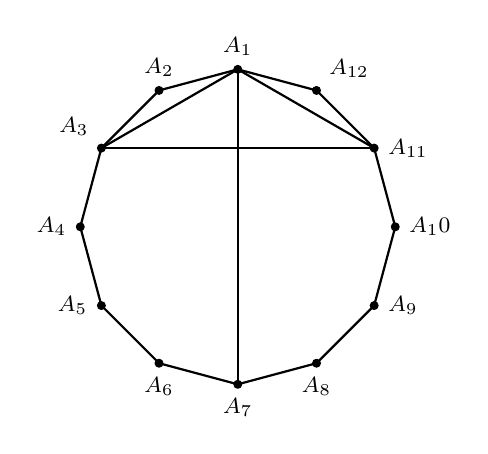
\begin{tikzpicture}[scale=1,>=stealth, font=\footnotesize, line join=round, line cap=round]
					\newdimen\R
					\R=2cm
					\draw[thick] (0:\R) \foreach \x in {30,60,90,...,360} { -- (\x:\R) };
					\foreach \x/\l/\p in
					{ 90/{$A_1$}/above,
						120/{$A_2$}/above,
						150/{$A_3$}/above left ,
						180/{$A_4$}/left,
						210/{$A_5$}/left,
						240/{$A_6$}/below,
						270/{$A_7$}/below,
						300/{$A_8$}/below,
						330/{$A_9$}/right,
						360/{$A_10$}/right,
						60/{$A_{12}$}/above right,
						30/{$A_{11}$}/right
					}
					\node[inner sep=1pt,circle,draw,fill,label={\p:\l}] at (\x:\R) {};
					\foreach \x/\l in{90/270,150/30,90/150,90/30} \draw[thick](\x:\R)--(\l:\R); 
				\end{tikzpicture}
			}
		}
	\end{vd}
\begin{vd}%[1D2G5-2]
	Cho đa giác đều $20 $ đỉnh. Lấy ngẫu nhiên $3$ đỉnh. Tính xác suất để $3$ đỉnh đó là $3$ đỉnh của $1$ tam giác vuông không cân.
	\loigiai
	{
		Chọn ngẫu nhiên $3$ đỉnh trong $20$ đỉnh có $\mathrm{C}_{20}^3$ cách $\Rightarrow n(\Omega)=1140$.\\
		Gọi $X$ là biến cố ``$3$ đỉnh đó là $3$ đỉnh của một tam giác vuông không cân''.\\
		Đa giác đều $20$ đỉnh có $10$ đường chéo đi qua tâm đa giác mà cứ $2$ đường chéo tạo thành $1$ hình chữ nhật và $1$ hình chữ nhật tạo thành $4$ tam giác vuông. Suy ra số tam giác vuông là $4\cdot \mathrm{C}_{10}^2=180$.\\
		Tuy nhiên, trong $\mathrm{C}_{10}^2$ hình chữ nhật có $5$ hình vuông nên số tam giác vuông cân là $5\cdot 4 = 20$.\\
		Do đó, số kết quả thuận lợi cho biến cố $X$ là $n(X)=180-20=160$.\\
		Vậy $P(X)=\dfrac{n(X)}{n(\Omega)}=\dfrac{160}{1140}=\dfrac{8}{57}.$
	}
\end{vd}

\begin{vd}%[1D2G5-2]
	Cho một đa giác đều có $18$ đỉnh nội tiếp trong một đường tròn tâm $O$. Gọi $X$ là tập hợp các tam giác có các đỉnh là các đỉnh của đa giác trên. Tính xác suất để chọn được một tam giác từ tập $X$ là tam giác cân nhưng không phải là tam giác đều.
	\loigiai
	{
		Chọn ngẫu nhiên $3$ đỉnh trong $18$ đỉnh có $\mathrm{C}_{18}^3$ cách.\\
		Gọi $X$ là biến cố ``tam giác được tạo từ $3$ đỉnh của đa giác là một tam giác cân nhưng không phải là tam giác đều ''.\\
		Gọi $1$ đỉnh $A$ của đa giác tạo với tâm $O$ một đường thẳng $AO$.\\
		Đường thẳng $AO$ này chia các đỉnh của đa giác thành $8$ cặp đỉnh đối xứng qua $AO$.
		Mỗi cặp đỉnh đối xứng tạo với $A$ một tam giác cân.\\
		Như vậy mỗi một đỉnh của đa giác tạo thành $8$ tam giác cân. Có $18$ đỉnh nên tạo thành $18\cdot 8 = 144$ tam giác cân.\\
		Tuy nhiên, trong $144$ tam giác cân này có $6$ tam giác đều. Do đó, số tam giác cân không phải tam giác đều là $n(X)=144-6=138$.\\
		Vậy $P(X)=\dfrac{n(X)}{n(\Omega)}=\dfrac{138}{\mathrm{C}_{18}^3}=\dfrac{23}{136}$.
	}
\end{vd}
\begin{vd}%[1D2G5-2]
	Cho đa giác đều $36$ đỉnh. Chọn ngẫu nhiên $4$ đỉnh trong $36$ đỉnh của đa giác. Tính xác suất để $4$ đỉnh được chọn tạo thành một hình vuông.
	\loigiai
	{
		Chọn ngẫu nhiên $4$ đỉnh trong $36$ đỉnh có $\mathrm{C}_{36}^4$ cách $\Rightarrow n(\Omega)=\mathrm{C}_{36}^4$.\\
		Gọi $X$ là biến cố ``$4$ đỉnh được chọn tạo thành một hình vuông''.\\
		Đa giác đều $36$ đỉnh tạo được $18$ đường chéo. Ứng với mỗi đường chéo sẽ có duy nhất một $1$ đường chéo trong $17$ đường chéo còn lại tạo thành $1$ hình vuông.\\
		Do đó $18$ đường chéo sẽ tạo được $18\colon 2=9$ hình vuông. Hay $n(X)=9$.\\
		Vậy $P(X)=\dfrac{9}{\mathrm{C}_{36}^4}= \dfrac{1}{6545}$.
	}
\end{vd}
	\begin{vd}%[1D2G5-2]
	Cho đa giác đều $32$ cạnh. Gọi $S$ là tập hợp các tứ giác tạo thành có $4$ đỉnh lấy từ các đỉnh của đa giác đều. Chọn ngẫu nhiên một phần tử của $S$. Tính xác suất để chọn được một hình chữ nhật.
	\loigiai{
		Gọi $(O)$ là đường tròn ngoại tiếp đa giác, do đa giác có số đỉnh là số chẳn nên đường nối một đỉnh tùy ý với tâm $O$ sẽ đi qua một đỉnh khác (ta gọi là $2$ điểm xuyên tâm đối).\\
		Do đa giác có $32$ đỉnh nên có $16$ cặp điểm xuyên tâm đối hay nói gọn hơn là có $16$ đường chéo đi qua tâm $O$.\\ 
		Với mỗi hai đường chéo qua tâm $O$ ta được $1$ hình chữ nhật.\\ 
		Vì có $12$ đường chéo nên số hình chữ nhật là: $\mathrm{C}_{16}^2=120$ .\\
		Số tứ giác tạo thành: $\mathrm{C}_{32}^4=35960$.\\
		Xác suất để chọn được một hình chữ nhật là $\dfrac{3}{899}$.}
\end{vd}
\baitaptl
\begin{bt}%[1D2B5-2]%
	Cho hai đường thẳng song song $d_1$ và $d_2$. Trên đường thẳng $d_1$ có $6$ điểm phân biệt được tô  màu đỏ, trên đường thẳng $d_2$ có $4$ điểm phân biệt được tô màu xanh. Xét tất cả các tam giác được tạo thành khi nối các điểm đó lại với nhau. Chọn ngẫu nhiên một tam giác, tính xác suất để thu được một tam giác có hai đỉnh màu đỏ.
	\loigiai{
		Chọn ngẫu nhiên một tam giác được tạo thành khi nối các điểm đó lại với nhau có $6\cdot \mathrm{C}_4^2+4\cdot \mathrm{C}_6^2=96$ cách.\\
		Vậy $n\left( \Omega\right) =96$.\\
		Gọi $A$ là biến cố ``thu được một tam giác có hai đỉnh màu đỏ''.\\
		Số kết quả thuận lợi của biến cố $A$ là $n\left( A\right)=4\cdot \mathrm{C}_6^2=60$.\\
		Xác suất của biến cố $A$ là $P\left( A\right)= \dfrac{60}{96}=\dfrac{5}{8}$.
	}
\end{bt}

\begin{bt}%[1D2B5-2]%
	Có $5$ đoạn thẳng có độ dài lần lượt là $1$ cm, $2$ cm, $3$ cm, $4$ cm, $5$ cm. Lấy ngẫu nhiên ba đoạn thẳng trong $5$ đoạn thẳng trên. Tính xác suất để ba đoạn thẳng lấy ra lập thành một tam giác. 
	\loigiai{
		Chọn ba đoạn thẳng trong $5$ đoạn thẳng có $\mathrm{C}_5^3=10$ cách. Suy ra $n\left( \Omega\right) =10$.\\ 
		Gọi $A$ là biến cố ``ba đoạn thẳng lấy ra lập thành một tam giác''.\\
		Ta có các bộ số sau thỏa yêu cầu bài toán là $\left(3;4;5 \right) $, $\left(2;3;4 \right) $, $\left(2;4;5 \right) $.\\
		Số kết quả thuận lợi của biến cố $A$ là $n\left( A\right)=3$.\\
		Xác suất của biến cố $A$ là $P\left( A\right)= \dfrac{3}{10}$.
	}
\end{bt}
\begin{bt}%[1D2B5-4]
	Cho đa giác đều $12$ đỉnh $A_1A_2...A_{12}$ nội tiếp đường tròn tâm $O$. Chọn ngẫu nhiên $4$ đỉnh của đa giác đó. Tính xác suất để bốn đỉnh được chọn tạo thành hình chữ nhật.
	\loigiai{
		Chọn bốn đỉnh trong $12$ đỉnh có $\mathrm{C}_{12}^4=495$ tứ giác. Suy ra $n\left( \Omega\right) =495$.\\ 
		Gọi $A$ là biến cố ``tứ giác được chọn là hình chữ nhật''.\\
		Số kết quả thuận lợi của biến cố $A$ là $n\left( A\right)=\mathrm{C}_{6}^2=15$.\\
		Xác suất của biến cố $A$ là $P\left( A\right)= \dfrac{15}{495}=\dfrac{1}{33}$.	
	}
\end{bt}

\begin{bt}%[1D2B5-4]
	Cho đa giác đều gồm $2n$ đỉnh $\left( n\geq2,\,n\in\mathbb{N}\right) $. Chọn ngẫu nhiên ba đỉnh trong số $2n$ đỉnh của đa giác, xác suất để ba đỉnh được chọn tạo thành một tam giác vuông là $0{,}2$. Tìm giá trị của $n$.
	\loigiai{
		Chọn ba đỉnh trong $2n$ đỉnh có $\mathrm{C}_{2n}^3$ tam giác. Suy ra $n\left( \Omega\right) =\mathrm{C}_{2n}^3$.\\ 
		Gọi $A$ là biến cố ``ba đỉnh được chọn là tam giác vuông''.\\
		Số kết quả thuận lợi của biến cố $A$ là $n\left( A\right)=n\cdot\left(2n-2 \right)$.\\
		Xác suất của biến cố $A$ là $P\left( A\right)= \dfrac{n\cdot\left(2n-2 \right)}{\mathrm{C}_{2n}^3}$.\\
		Theo đề bài ta có
		\begin{eqnarray*}
			\dfrac{n\cdot\left(2n-2 \right)}{\mathrm{C}_{2n}^3}=0{,}2&\Leftrightarrow& n\cdot\left(2n-2 \right)=\dfrac{0{,}2}{6}\cdot \left( 2n-2\right) \cdot \left( 2n-1\right)\cdot 2n\\&\Leftrightarrow& \left(2n-2 \right)\left( 30n-4n^2+2n\right)=0\\&\Leftrightarrow& \hoac{&n=1\\&n=8\\&n=0.}\\&\Leftrightarrow& n=8.	
		\end{eqnarray*}	
	}
\end{bt}
	\begin{bt}%[1D2G5-4]
	Chọn ngẫu nhiên ba đỉnh từ các đỉnh của một đa giác đều nội tiếp đường tròn tâm $O$, biết đa giác có $170$ đường chéo. Tính xác suất $P$ của biến cố chọn được ba đỉnh sao cho ba đỉnh được chọn tạo thành một tam giác vuông không cân.
	\loigiai{
		Gọi $n$ là số đỉnh của đa giác đều $(n \in \mathbb{N^*})$. Ta đi tìm số đường chéo của đa giác đều.\\
		Số cách chọn $2$ đỉnh từ $n$ đỉnh là $\mathrm{C}_n^2$.
		Do đó số đường chéo của đa giác đều bằng $\mathrm{C}_n^2-n=170$.\\
		\begin{eqnarray*}
		\dfrac{n!}{2!(n-2)!}-n=170 \Leftrightarrow \dfrac{n^2-n}{2}-n=170 \\ \Leftrightarrow n^2-3n-340=0 \\ \Leftrightarrow \hoac{&n=20 \text{ (nhận)}\\&n=-17 \text{ (loại).}}	
		\end{eqnarray*}	
		Số phần tử của không gian mẫu: Chọn $3$ đỉnh từ $20$ đỉnh có $\mathrm{C}_{20}^3=1140$ cách.\\
		Gọi $A$ là biến cố: Ba đỉnh được chọn tạo thành một tam giác vuông không cân.
		\begin{itemize}
			\item Để $3$ đỉnh được chọn là tam giác vuông ta cần chọn cạnh huyền từ $10$ đường kính của đường tròn tâm $O$: có $10$ cách.
			\item Sau khi chọn được cạnh huyền của tam giác vuông ta còn lại $18$ đỉnh, (giả sử đó là đỉnh thứ $1$ và thứ $11$ của đa giác đều) ta cần chọn điểm còn lại để tạo thành tam giác vuông không cân. Cần chọn các đỉnh khác với đỉnh thứ $6$ và $16$, suy ra có $16$ cách chọn.
			\item Số cách chọn để ba đỉnh tạo thành một tam giác vuông không cân là $10\cdot 16=160$ cách.
		\end{itemize}
		Vậy $\mathrm{P}(A)=\dfrac{160}{1140}=\dfrac{8}{57}$.
	}
\end{bt}	
\begin{bt}%[1D2G5-2]
	Cho một đa giác đều có 18 đỉnh nội tiếp trong một đường tròn tâm $O$. Gọi $X$ là tập các tam giác có các đỉnh là các đỉnh của của đai giác trên. Tính xác suất để chọn được một tam giác từ tập $X$ là tam giác cân nhưng không phải là tam giác đều. 
	\loigiai{
		\immini{
			
			Qua ba đỉnh của đa giác luôn tạo thành một tam giác nên số tam giác có ba đỉnh là ba đỉnh của đa giác là $n\left (\Omega\right ) =\mathrm{C}_{18}^3$.
			
			
			Có $18$ cách chọn một đỉnh của đa giác mỗi đỉnh có $7$ cách chọn $2$ đỉnh còn lại để được một tam giác cân không đều.
			
			Số các tam giác cân không đều là $18.7 =126.$
			
			Xác suất cần tìm $P(A) =\dfrac{128}{\mathrm{C}_{18}^3} =\dfrac{21}{136}.$}
		{
			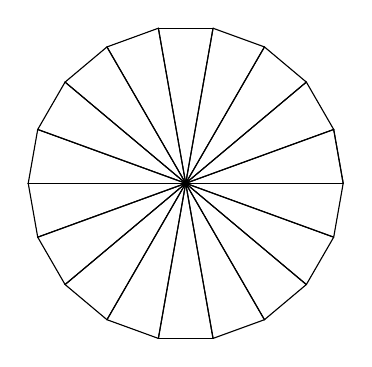
\begin{tikzpicture}[scale=1,>=stealth, font=\footnotesize, line join=round, line cap=round]
				\foreach \x in {0,20,...,360} {
					\draw[fill] (\x:2 cm) -- (\x + 20:2 cm);
					\draw[fill] (\x:2 cm) -- (\x + 180:2 cm);}
		\end{tikzpicture}}
	}
\end{bt}
\begin{bt}%[1D2G5-2]
	Cho đa giác đều gồm $2018$ đỉnh $A_1A_2\ldots A_{2018}$. Chọn ngẫu nhiên ra $3$ đỉnh trong $2018$ đỉnh của đa giác, xác suất để $3$ đỉnh được chọn là $3$ đỉnh của một tam giác tù là bao nhiêu?
	\loigiai{
		Chọn $3$ đỉnh ngẫu nhiên ta có $\mathrm{C}^3_{2018}$ cách chọn.\\
		Suy ra $| \Omega | = \mathrm{C}^3_{2018}$.\\
		Gọi $A$ là biến cố để chọn được $3$ đỉnh là $3$ đỉnh của một tam giác tù.\\
		Giả sử chọn tam giác tù $ABC$ với $A$ nhọn, $B$ tù và $C$ nhọn.\\
		Chọn một đỉnh bất kì làm đỉnh $A$ suy ra có $2018$ cách chọn.\\
		Qua đỉnh vừa chọn, ta kẻ đường kính, chia đa giác làm hai phần.\\
		Để tạo thành tam giác tù thì hai đỉnh $B$ và $C$ sẽ phải cùng nằm về một phía.\\
		Suy ra có $\mathrm{C}^2_{1008}+\mathrm{C}^2_{1008} = 2\mathrm{C}^2_{1008}$.\\
		Vì vai trò của $A$, $C$ như nhau nên mỗi tam giác được tính hai lần.\\
		Do vậy $|A|= 2018 \cdot \mathrm{C}^2_{1008}$.\\ Suy ra $P(A)= \dfrac{2018 \cdot 2 \cdot \mathrm{C}^2_{1008}}{\mathrm{C}_3^{2018}}=\dfrac{3021}{4034}$.
	}
\end{bt}	
	
% \begin{dang}{Các bài toán bàn tròn}
% 	Có $n$ phần tử được sắp xếp trên một vòng tròn $n$ vị trí. Số cách xếp sẽ là hoán vị của $n-1$ phần tử: $(n-1)!$.
% \end{dang}
% \viduminhhoa
% \begin{vd}%[1D2B2]
% 	Tính xác suất để $5$ bạn nam và $5$ bạn nữ ngồi xung quanh một bàn tròn sao cho nam và nữ ngồi xen kẽ với nhau.
% 	\loigiai{Số phần tử của không gian mẫu là $ n\left(\Omega\right)=9! $.\\
% 		Chọn $1$ bạn nam ngồi cố định vào $ 1 $ vị trí, $9$ bạn còn lại sẽ hoán vị xung quanh bạn này theo nguyên tắc là nam nữ xen kẽ. Khi đó, các bạn nam còn lại sẽ ở vị trí mang số $3,5,7,9$ và nữ sẽ ở vị trí số $2,4,6,8,10$ (theo chiều kim đồng hồ). Ở mỗi vị trí của mình, các nam và nữ được hoán vị cho nhau.
% 		Do đó, có $1\cdot4!\cdot 5!=2.880$ cách sắp xếp.\\
% 		Gọi $A$ là biến cố : ``$5$ bạn nam và $5$ bạn nữ ngồi xen kẽ với nhau trên một bàn tròn''.\\
% 		Ta có $\mathrm{P}(A)=\dfrac{n(A)}{n(\Omega)}=\dfrac{2880}{9!}$.
% 	}
% \end{vd}	
% \begin{vd}%[1D2K2]
% 	Tính xác suất để $ 5 $ bạn nữ và $ 3 $ bạn nam thành $ 1 $ vòng tròn sao cho mỗi nam phải đứng giữa $ 2 $ nữ bất kỳ.
% 	\loigiai{Số phần tử của không gian mẫu là $ n\left(\Omega\right)=7! $.\\
% 		Chọn $1$ nữ cố định, ta xếp $4$ nữ còn lại quanh vòng tròn thì giữa $5$ nữ này có $5$ chỗ trống. Chỉ cần đặt $3$ nam vào $3$ trong $5$ vị trí này thì được ngay một cách xếp.	Khi đó, có $4!\cdot \mathrm{A}^3_5=1440$ cách.\\
% 		Gọi $A$ là biến cố: ``$ 5 $ bạn nữ và $ 3 $ bạn nam thành $ 1 $ vòng tròn sao cho mỗi nam phải đứng giữa $ 2 $ nữ bất kỳ.\\
% 			Ta có $\mathrm{P}(A)=\dfrac{n(A)}{n(\Omega)}=\dfrac{1440}{7!}$.
% 	}
% \end{vd}
% 	\begin{vd}%[1D2K2-4]
% 	Lớp 10A4 cử đại diện $3$ học sinh, 11A5 cử đại diện $4$ học sinh, 12A6 cử đại diện $5$ học sinh đi đại hội (ngồi bàn tròn). Hỏi xác suất các thành viên của mỗi lớp ngồi cạnh nhau là bao nhiêu?

% 	\loigiai{
% 		Số phần tử của không gian mẫu là $ n\left(\Omega\right)=11! $.\\
% 		\begin{itemize}
% 			\item Xem $3$ học sinh lớp $10$ là $X$; $4$ học sinh lớp $11$ là $Y$; $5$ học sinh lớp $12$ là $Z$.
% 			\item Xếp $X$, $Y$, $Z$ vào bàn tròn có $2$ cách. Khi đó, $X$ có $3!$, $Y$ có $4!$, $Z$ có $5!$ cách sắp xếp.
% 			\item Vậy có $2\cdot 3!\cdot 4!\cdot 5!$ cách sắp xếp.
% 		\end{itemize}
% 	Gọi $A$ là biến cố: ``các thành viên của mỗi lớp ngồi cạnh nhau''.\\
%  Ta có $\mathrm{P}(A)=\dfrac{n(A)}{n(\Omega)}=\dfrac{2\cdot 3!\cdot 4!\cdot 5!}{11!}$.
% 	}
% \end{vd}

% 	\begin{vd}%[1D2G5-2]
% 	Xếp $6$ học sinh nam và $ 4 $ học sinh nữ ngồi vào một bàn tròn $10$ ghế. Tính xác suất để không có hai học sinh nữ ngồi cạnh nhau. 
% 	\loigiai{
% 		Chọn một học sinh ngồi cố định vào bàn tròn. Khi đó, có $ 9! $ cách sắp xếp các học sinh còn lại vào bàn tròn. Do đó, số phần tử của không gian mẫu là $ n\left(\Omega\right)=9! $.\\
% 		Gọi $ A $ là biến cố \lq\lq không có hai học sinh nữ ngồi cạnh nhau\rq\rq.\\
% 		Với một học sinh nam ngồi cố định vào bàn tròn, khi đó
% 		\begin{itemize}
% 			\item có $ 5! $ cách sắp xếp $ 5 $ học sinh nam còn lại vào bàn tròn sao cho có thể linh động chừa khoảng trống để học sinh nữ ngồi. Như vậy có tất cả $ 6 $ khoảng trống giữa các học sinh nam,
% 			\item có $ \mathrm{A}_6^4 $ cách sắp xếp $ 4 $ học sinh nữ vào $ 6 $ khoảng trống giữa các học sinh nam.
% 		\end{itemize}
% 		Như thế, số phần tử thuận lợi cho biến cố $ A $ là $ n(A)=5!\times \mathrm{A}_6^4$.\\
% 		Vậy xác suất cần tìm là $ \mathrm{P}(A)=\dfrac{n(A)}{n(\Omega)}=\dfrac{5!\times\mathrm{A}_6^4}{9!}=\dfrac{5}{42} $.
% 	}
% \end{vd}
% 	\begin{vd}%[1D2K2-4]
% 	Tính xác suất khi xếp $3$ người đàn ông, $2$ người đàn bà và $1$ đứa trẻ ngồi vào ghế xếp quanh một bàn tròn sao cho đứa trẻ ngồi giữa hai người đàn ông.
% 	\loigiai{
% 		Số phần tử của không gian mẫu là $n\left(\Omega\right)=5! $.\\
% 		Chọn $2$ người đàn ông có $\mathrm{C}_3^2=3$ cách.\\
% 		Xếp $2$ người đó ngồi cạnh nhau có $2$ cách.\\
% 		Xếp đứa trẻ vào giữa $2$ người này có $1$ cách.\\
% 		Xếp $3$ người còn lại vào $3$ ghế còn lại có $3!=6$ cách.\\
% 		Vậy có tất cả $3\cdot 2 \cdot 1 \cdot 6=36$ cách.\\
% 		Gọi $\mathrm{A}$ là biến cố: ``đứa trẻ ngồi giữa hai người đàn ông''.\\
% 		Ta có $\mathrm{P}(A)=\dfrac{n(A)}{n(\Omega)}=\dfrac{36}{5!}.$
% 	}
% \end{vd}
% \baitaptl
% \setcounter{bt}{0}
% 	\begin{bt}%[1D2B2-4]
% 	Tính xác suất khi xếp $6$ người quanh bàn tròn sao cho có một cặp vợ chồng ngồi cạnh nhau.
% 	\loigiai{
% 		Số phần tử của không gian mẫu là $n\left(\Omega\right)=5! $.\\
% 		Xem như cặp vợ chồng là một nhóm. Số cách xếp $1$ nhóm và $4$ người vào bàn tròn là $4!$ cách.\\
% 		Số cách xếp $2$ vợ chồng trong nhóm là $2!$ cách.\\
% 		Vậy có $2!\cdot 4!$ cách xếp.\\
% 		Gọi $\mathrm{A}$ là biến cố: ``một cặp vợ chồng ngồi cạnh nhau''.\\
% 		Ta có $\mathrm{P}(A)=\dfrac{n(A)}{n(\Omega)}=\dfrac{2!\cdot 4!}{5!}.$ 
% 	}
% \end{bt}
% 	\begin{bt}%[1D2K2-4]
% 	Có $4$ người đàn ông, $2$ người đàn bà và $1$ đứa trẻ được xếp ngồi vào bảy chiếc ghế đặt quanh một bàn tròn. Tính xác suất sao cho
% 	\begin{enumerate} 
% 		\item đứa trẻ ngồi giữa hai người đàn bà.
% 		\item đứa trẻ ngồi giữa hai người đàn ông.
% 	\end{enumerate}
% 	\loigiai{Số phần tử của không gian mẫu là $n\left(\Omega\right)=6! $.
% 		\begin{enumerate} 
% 			\item 
% 			\begin{itemize}
% 				\item Bước 1: Chọn $1$ ghế xếp em bé có $1$ cách (vì ngồi xung quanh bàn tròn).
% 				\item Bước 2: Xếp $2$ người phụ nữ ngồi $2$ ghế kề em bé, có $2!$ cách.
% 				\item Bước 3: Xếp $4$ người đàn ông vào $4$ ghế còn lại, có $4!$ cách.
% 			\end{itemize}
% 			Theo quy tắc nhân, có $2!\cdot 4!=48$ cách xếp.\\
% 			Gọi $\mathrm{A}$ là biến cố: ``đứa trẻ ngồi giữa hai người đàn bà''.\\
% 			Ta có $\mathrm{P}(A)=\dfrac{n(A)}{n(\Omega)}=\dfrac{48}{6!}.$
% 			\item 
% 			\begin{itemize}
% 				\item Bước 1: Chọn $2$ người đàn ông trong $4$ người, có $\mathrm{C}_4^2$ cách.
% 				\item Bước 2: Chọn $1$ ghế xếp em bé, có $1$ cách (vì ngồi xung quanh bàn tròn).
% 				\item Bước 3: Xếp $2$ người đàn ông vừa chọn ngồi 2 ghế kề em bé, có $2!$ cách.
% 				\item Bước 4:  Xếp $4$ người còn lại vào $4$ ghế còn lại, có $4!$ cách.
% 			\end{itemize}
% 			Theo quy tắc nhân có $\mathrm{C}_4^2\cdot 2!\cdot 4!=288$ cách xếp.\\
% 			Gọi $\mathrm{B}$ là biến cố: ``đứa trẻ ngồi giữa hai người đàn ông''.\\
% 			Ta có $\mathrm{P}(A)=\dfrac{n(B)}{n(\Omega)}=\dfrac{288}{6!}.$
% 		\end{enumerate}	
% 	}
% \end{bt}
% \begin{bt}%[1D2K2-4]
% 	Tính xác suất sao cho
% 		\begin{itemize}
% 		\item  khi xếp $6$ cặp vợ chồng ngồi xung quanh một chiếc bàn tròn thì nam và nữ xen kẽ nhau.
% 		\item  khi xếp $6$ cặp vợ chồng ngồi xung quanh một chiếc bàn tròn thì mỗi bà đều ngồi cạnh chồng của mình. 
% 	\end{itemize}
% 	\loigiai{Số phần tử của không gian mẫu là $n\left(\Omega\right)=11! $.\\	
% 		\begin{itemize}
% 			\item  Ta tiến hành xếp chỗ ngồi theo hai công đoạn.\\
% 			\textbf{Bước 1.} Xếp $6$ nam ngồi quanh bàn tròn, có $5!$ cách xếp.\\
% 			\textbf{Bước 2.} Ta xem 6 người nam vừa xếp là $6$ vách ngăn, vì $6$ người nam ngồi quanh bàn tròn nên có $6$ khoảng trống để xếp $6$ người nữa, vậy có $6!$ cách xếp.\\
% 			Theo quy tắc nhân ta có $5!\cdot 6!=86400$ cách.\\
% 			Gọi $\mathrm{A}$ là biến cố: ``nam và nữ ngồi xen kẽ nhau''.\\
% 			Ta có $\mathrm{P}(A)=\dfrac{n(A)}{n(\Omega)}=\dfrac{86400}{11!}.$
% 			\item  Ta tiến hành xếp chỗ ngồi theo hai công đoạn.\\
% 			\textbf{Bước 1.} Xếp $6$ người chồng ngồi quanh bàn tròn, có $5!$ cách xếp, vì vợ ngồi gần chồng.\\
% 			\textbf{Bước 2.} Mỗi cặp vợ chồng đổi chỗ cho nhau có $1$ cách xếp mới, vậy có $2^6$ cách.\\
% 			Theo quy tắc nhân có $5! \cdot 2^6=7680$ cách.\\
% 			Gọi $\mathrm{B}$ là biến cố: ``mỗi bà đều ngồi cạnh chồng mình''.\\
% 			Ta có $\mathrm{P}(A)=\dfrac{n(A)}{n(\Omega)}=\dfrac{7680}{11!}.$
% 		\end{itemize}
% 	}
% \end{bt}



\subsection{Bài tập trắc nghiệm cuối bài}
\setcounter{ex}{0}
\Opensolutionfile{ans}[ans/ans-xs]
\Opensolutionfile{ansbook}[ans/ansbook-xs]
\begin{ex}%[1D2B5-2]
	Có $7$ tấm bìa ghi $7$ chữ \rq\rq HIỀN \lq\lq, \lq\lq TÀI \lq\lq, \lq\lq LÀ \lq\lq, \lq\lq NGUYÊN \lq\lq, \lq\lq KHÍ \lq\lq, \lq\lq QUỐC \lq\lq, \lq\lq GIA \lq\lq. Một người xếp ngẫu nhiên $7$ tấm bìa cạnh nhau. Tính xác suất để khi xếp các tấm bìa được dòng chữ \lq\lq HIỀN TÀI LÀ NGUYÊN KHÍ QUỐC GIA \lq\lq. 
	\choice
	{$\dfrac{1}{25}$}
	{\True $\dfrac{1}{5040}$}
	{$\dfrac{1}{24}$}
	{$\dfrac{1}{13}$}
	\loigiai{
		Xếp ngẫu nhiên $7$ tấm bìa có $7!=5040$ (cách xếp) $\Rightarrow n(\Omega)=5040$.\\
		Đặt $A$ là biến cố \lq\lq xếp được chữ HIỀN TÀI LÀ NGUYÊN KHÍ QUỐC GIA \lq\lq. Ta có $n(A)=1$.\\
		Vậy $\mathrm{P}(A)=\dfrac{1}{5040}$.}
\end{ex}

\begin{ex}%[1D2B5-2]
	Trên giá sách có $4$ quyển sách toán, $3$ quyển sách lý, $2$ quyển sách hóa. Lấy ngẫu nhiên $3$ quyển sách. Tính xác suất để trong ba quyển sách lấy ra có ít nhất một quyển là toán. 
	\choice
	{$\dfrac{2}{7}$}
	{$\dfrac{3}{4}$}
	{\True $\dfrac{37}{42}$}
	{$\dfrac{10}{21}$}
	\loigiai{
		Số kết quả có thể khi chọn bất kì $3$ quyển sách trong $9$ quyển sách là $\mathrm{C}_9^3=84$.\\
		Gọi $A$ là biến cố \lq\lq Lấy được ít nhất $1$ sách toán trong $3$ quyển sách \lq\lq.\\
		$\overline{A}$ là biến cố \lq\lq Không lấy được sách toán trong $3$ quyển sách \lq\lq.\\
		Ta có xác sút để xảy ra $A$ là $\mathrm{P}(A)=1-\mathrm{P}\left(\overline{A}\right)=1-\dfrac{\mathrm{C}_5^3}{84}=\dfrac{37}{42}$.}
\end{ex}

\begin{ex}%[1D2B5-2]
	Gieo ngẫu nhiên $2$ con xúc sắc cân đối đồng chất. Tìm xác suất của biến cố$\colon$ \lq\lq Hiệu số chấm xuất hiện trên $2$ con xúc sắc bằng $1$ \lq\lq. 
	\choice
	{$\dfrac{2}{9}$}
	{$\dfrac{1}{9}$}
	{\True $\dfrac{5}{18}$}
	{$\dfrac{5}{6}$}
	\loigiai{
		Số phần tử của không gian mẫu$\colon$ $n(\Omega)=6\cdot 6=36$.\\
		Gọi $A$ là biến cố thỏa mãn yêu cầu bài toán$\colon$\\
		$A=\left\{(1; 2),(2; 1),(3; 2),(2; 3),(3; 4),(4; 3),(4; 5),(5; 4),(5; 6),(6; 5)\right\}$ nên $n(A)=10$.\\
		Vậy $\mathrm{P}(A)=\dfrac{10}{36}=\dfrac{5}{18}$.}
\end{ex}

\begin{ex}%[1D2B5-2]
	Có $10$ tấm bìa ghi 10 chữ \lq\lq NƠI \lq\lq, \lq\lq NÀO \lq\lq, \lq\lq CÓ \lq\lq, \lq\lq Ý \lq\lq, \lq\lq CHÍ \lq\lq, \lq\lq NƠI \lq\lq, \lq\lq ĐÓ \lq\lq, \lq\lq CÓ \lq\lq, \lq\lq CON \lq\lq, \lq\lq ĐƯỜNG \lq\lq. Một người xếp ngẫu nhiên 10 tấm bìa cạnh nhau. Tính xác suất để xếp các tấm bìa được dòng chữ \lq\lq NƠI NÀO CÓ Ý CHÍ NƠI ĐÓ CÓ CON ĐƯỜNG \lq\lq. 
	\choice
	{$\dfrac{1}{40320}$}
	{$\dfrac{1}{10}$}
	{$\dfrac{1}{3628800}$}
	{\True $\dfrac{1}{907200}$}
	\loigiai{
		Số phần tử của không gian mẫu là $n(\Omega)=10!$.\\
		Gọi $A$ là biến cố xếp các tấm bìa được dòng chữ \lq\lq NƠI NÀO CÓ Ý CHÍ NƠI ĐÓ CÓ CON ĐƯỜNG \lq\lq.\\
		Chú ý rằng có hai chữ \lq\lq NƠI \lq\lq và hai chữ \lq\lq CÓ \lq\lq, nên để tính $n(A)$, ta làm như sau
		\begin{itemize}
			\item Có $\mathrm{C}_2^1$ cách chọn một chữ \lq\lq NƠI \lq\lq và đặt vào đầu câu.
			\item Có $\mathrm{C}_2^1$ cách chọn một chữ \lq\lq CÓ \lq\lq và đặt vào vị trí thứ ba.
			\item Các vị trí còn lại chỉ có một cách đặt chữ.
			\item Vậy $n(A)=\mathrm{C}_2^1\cdot\mathrm{C}_2^1\cdot 1=4$, nên $\mathrm{P}(A)=\dfrac{4}{10!}=\dfrac{4}{3628800}=\dfrac{1}{907200}$.
		\end{itemize}
	}
\end{ex}

\begin{ex}%[1D2B5-2]
	Một lô hàng gồm $30$ sản phẩm tốt và $10$ sản phẩm xấu. Lấy ngẫu nhiên $3$ sản phẩm. Tính xác suất để $3$ sản phẩm lấy ra có ít nhất một sản phẩm tốt. 
	\choice
	{$\dfrac{135}{988}$}
	{$\dfrac{3}{247}$}
	{\True $\dfrac{244}{247}$}
	{$\dfrac{15}{26}$}
	\loigiai{
		Chọn ra ba sản phẩm tùy ý có $\mathrm{C}_{40}^3=9880$ cách Do đó $n(\Omega)=9880$.\\
		Gọi $A$ là biến cố có ít nhất $1$ sản phẩm tốt. Khi đó $\overline{A}$ là biến cố 3 sản phẩm không có sản phẩm tốt.\\
		$n\left(\overline{A}\right)=\mathrm{C}_{10}^3=120$.\\
		Vậy xác suất cần tìm là $\mathrm{P}(A)=1-\mathrm{P}\left(\overline{A}\right)=1-\dfrac{n\left(\overline{A}\right)}{n(\Omega)}=1-\dfrac{120}{9880}=\dfrac{244}{247}$.}
\end{ex}

\begin{ex}%[1D2B5-2]
	Trong trò chơi “Chiếc nón kỳ diệu” chiếc kim của bánh xe có thể dừng lại ở một trong $6$ vị trí với khả năng như nhau. Tính xác suất để trong ba lần quay, chiếc kim của bánh xe đó lần lượt dừng lại ở ba vị trí khác nhau. 
	\choice
	{$\dfrac{5}{36}$}
	{\True $\dfrac{5}{9}$}
	{$\dfrac{5}{54}$}
	{$\dfrac{1}{36}$}
	\loigiai{
		Số phần tử của không gian mẫu là $n(\Omega)=\mathrm{C}_6^1\mathrm{C}_6^1\mathrm{C}_6^1=6^3$.\\
		Gọi A là biến cố “trong ba lần quay, chiếc kim của bánh xe dừng lại ở ba vị trí khác nhau”.\\
		Số phần tử thuận lợi cho biến cố $A$ là $n(A)=\mathrm{C}_6^1\mathrm{C}_5^1\mathrm{C}_4^1$.\\
		Vậy xác suất của biến cố $A$ là $\mathrm{P}(A)=\dfrac{n(A)}{n(\Omega)}=\dfrac{\mathrm{C}_6^1\mathrm{C}_5^1\mathrm{C}_4^1}{\mathrm{C}_6^1\mathrm{C}_6^1\mathrm{C}_6^1}=\dfrac{5}{9}$.}
\end{ex}

\begin{ex}%[1D2B5-2]
	Lấy ngẫu nhiên hai viên bi từ một thùng gồm $4$ bi xanh, $5$ bi đỏ và $6$ bi vàng. Tính xác suất để lấy được hai viên bi khác màu?
	\choice
	{$67{,}6\%$}
	{$29{,}5\%$}
	{$32{,}4\%$}
	{\True $70{,}5\%$}
	\loigiai{
		Tổng số bi trong thùng là $4+5+6=15$ (bi).\\
		Số kết quả có thể khi lấy ra $2$ viên bi bất kì từ $15$ viên bi là $\mathrm{C}_{15}^2=105$.\\
		Số kết quả thuận lợi khi lấy ra hai bi khác màu là $\mathrm{C}_4^1\mathrm{C}_5^1+\mathrm{C}_5^1\mathrm{C}_6^1+\mathrm{C}_4^1\mathrm{C}_6^1=74$.\\
		Gọi $A$ là biến cố lấy ra hai viên bi khác màu. Xác suất xảy ra $A$ là $\mathrm{P}(A)=\dfrac{74}{105}\simeq 70{,}5\%$.}
\end{ex}

\begin{ex}%[1D2B5-2]
	Thầy giáo có $10$ câu hỏi trắc nghiệm, trong đó có $6$ câu đại số và $4$ câu hình học. Thầy gọi bạn Nam lên trả bài bằng cách chọn lấy ngẫu nhiên $3$ câu hỏi trong $10$ câu hỏi trên để trả lời. Hỏi xác suất bạn Nam chọn ít nhất có một câu hình học là bằng bao nhiêu?
	\choice
	{\True $\dfrac{5}{6}$}
	{$\dfrac{1}{30}$}
	{$\dfrac{1}{6}$}
	{$\dfrac{29}{30}$}
	\loigiai{
		Chọn ngẫu nhiên $3$ câu hỏi trong $10$ câu hỏi thì số phần tử của không gian mẫu $\colon n(\Omega)=\mathrm{C}_{10}^3$.\\
		Gọi $A\colon$ \lq\lq chọn ít nhất có một câu hình học \lq\lq, suy ra $\overline{A}\colon$ \lq\lq không chọn được câu hình \lq\lq.\\
		Có $n\left(\overline{A}\right)=\mathrm{C}_6^3$ suy ra $\mathrm{P}(A)=1-\mathrm{P}\left(\overline{A}\right)=1-\dfrac{\mathrm{C}_6^3}{\mathrm{C}_{10}^3}=\dfrac{5}{6}$.}
\end{ex}

\begin{ex}%[1D2B5-2]
	Để chào mừng ngày nhà giáo Việt Nam $20-11$ Đoàn trường THPT Hai Bà Trưng đã phân công ba khối$\colon$ khối $10$, khối $11$ và khối $12$ mỗi khối chuẩn bị ba tiết mục gồm$\colon$ một tiết mục múa, một tiết mục kịch và một tiết mục hát tốp ca. Đến ngày tổ chức ban tổ chức chọn ngẫu nhiên ba tiết mục. Tính xác suất để ba tiết mục được chọn có đủ ba khối và có đủ ba nội dung?
	\choice
	{\True $\dfrac{1}{14}$}
	{$\dfrac{1}{84}$}
	{$\dfrac{1}{28}$}
	{$\dfrac{9}{56}$}
	\loigiai{
		Chọn ba tiết mục trong chín tiết mục có $n(\Omega)=\mathrm{C}_9^3$ cách chọn.\\
		Gọi $A$ là biến cố$\colon$ ba tiết mục được chọn có đủ ba khối và có đủ ba nội dung.\\
		Chọn tiết mục khối $10$ có $3$ cách chọn.\\
		Chọn tiết mục ở khối $11$ có $2$ cách.\\
		Và tiết mục ở khối $12$ có 1 cách.\\
		Nên có $n(A)=3\cdot 2\cdot 1=6$ cách chọn.\\
		Xác suất của biến cố $A\colon$ $\mathrm{P}(A)=\dfrac{n(A)}{n(\Omega)}=\dfrac{1}{14}$.}
\end{ex}

\begin{ex}%[1D2B5-2]
	Kết quả $(b,c)$ của việc gieo con xúc sắc cân đối và đồng chất hai lần, trong đó $b$ là số chấm xuất hiện trong lần gieo đầu, $c$ là số chấm xuất hiện ở lần gieo thứ hai, được thay vào phương trình bậc hai $x^2+bx+c=0$. Tính xác suất để phương trình có nghiệm. 
	\choice
	{\True $\dfrac{19}{36}$}
	{$\dfrac{1}{2}$}
	{$\dfrac{1}{18}$}
	{$\dfrac{17}{36}$}
	\loigiai{
		Xét biến cố $A$$\colon$ \lq\lq phương trình có nghiệm \lq\lq.\\
		Trường hợp 1$\colon$ $b\geq 5$. Khi đó $c$ nhận giá trị tùy ý, nên có tất cả $2.6=12$ kết quả thuận lợi cho biến cố $A$.\\
		Trường hợp 2$\colon$ $b=4$. Khi đó $c\leq 4$, nên có $1.4=4$ kết quả thuận lợi cho biến cố $A$.\\
		Trường hợp 3$\colon$ $b<4$. Có $3$ kết quả là $(3,1)$, $(3,2)$, $(2,1)$.\\
		Vậy $n(A)=12+4+3=19$.\\
		Xác suất để phương trình có nghiệm là $\mathrm{P}(A)=\dfrac{19}{36}$.}
\end{ex}

\begin{ex}%[1D2B5-2]
	Một tổ có $9$ học sinh nam và $3$ học sinh nữ. Chia tổ thành $3$ nhóm, mỗi nhóm $4$ người để làm $3$ nhiệm vụ khác nhau. Tính xác suất khi chia ngẫu nhiên nhóm nào cũng có nữ. 
	\choice
	{$\dfrac{8}{55}$}
	{$\dfrac{292}{34650}$}
	{$\dfrac{292}{1080}$}
	{\True $\dfrac{16}{55}$}
	\loigiai{
		Không gian mẫu $\mathrm{C}_{12}^4\mathrm{C}_8^4\cdot 1=34650$.\\
		Gọi $A$ là biến cố \lq\lq Chia mỗi nhóm có đúng một nữ và ba nam \lq\lq.\\
		Số cách phân chia cho nhóm $1$ là $\mathrm{C}_3^1\mathrm{C}_9^3=252$ (cách).\\
		Khi đó còn lại $2$ nữ $6$ nam nên số cách phân chia cho nhóm $2$ có $\mathrm{C}_2^1\mathrm{C}_6^3=40$ (cách).\\
		Cuối cùng còn lại bốn người thuộc về nhóm $3$ nên có $1$ cách Theo quy tắc nhân ta có số kết quả thuận lợi $n(A)=252\cdot 40\cdot 1=10080$ (cách).\\
		Vậy xác suất cần tìm là $\mathrm{P}(A)=\dfrac{10080}{34650}=\dfrac{16}{55}$.}
\end{ex}

\begin{ex}%[1D2B5-2]
	Một lớp có 20 nam sinh và 15 nữ sinh. Giáo viên chọn ngẫu nhiên 4 học sinh lên bảng giải bài tập. Tính xác suất để 4 học sinh được chọn có cả nam và nữ. 
	\choice
	{\True $\dfrac{4615}{5236}$}
	{$\dfrac{4651}{5236}$}
	{$\dfrac{4615}{5263}$}
	{$\dfrac{4610}{5236}$}
	\loigiai{
		Số cách chọn $4$ học sinh lên bảng$\colon$ $n(\Omega)=\mathrm{C}_{35}^4$.\\
		Số cách chọn $4$ học sinh chỉ có nam hoặc chỉ có nữ$\colon$ $\mathrm{C}_{20}^4+\mathrm{C}_{15}^4$.\\
		Xác suất để $4$ học sinh được gọi có cả nam và nữ$\colon$ $1-\dfrac{\mathrm{C}_{20}^4+\mathrm{C}_{15}^4}{\mathrm{C}_{35}^4}=\dfrac{4615}{5236}$.}
\end{ex}

\begin{ex}%[1D2B5-2]
	Một cái hộp chứa $6$ viên bi đỏ và $4$ viên bi xanh. Lấy lần lượt $2$ viên bi từ cái hộp đó. Tính xác suất để viên bi được lấy lần thứ $2$ là bi xanh. 
	\choice
	{\True $\dfrac{2}{5}$}
	{$\dfrac{7}{24}$}
	{$\dfrac{11}{12}$}
	{$\dfrac{7}{9}$}
	\loigiai{
		Ta có Số phần tử của không gian mẫu $n(\Omega)=\mathrm{C}_{10}^1\cdot\mathrm{C}_9^1$.\\
		Gọi $A$ là biến cố $\colon$ \lq\lq Viên bi được lấy lần thứ $2$ là bi xanh \lq\lq.
		\begin{itemize}
			\item Trường hợp 1 $\colon$ Lần 1 lấy viên đỏ, lần 2 lấy viên xanh $\colon$ Có $\mathrm{C}_6^1\cdot\mathrm{C}_4^1$ cách chọn.
			\item Trường hợp 2 $\colon$ Lần 1 lấy viên xanh, lần 2 lấy viên xanh $\colon$ Có $\mathrm{C}_4^1\cdot\mathrm{C}_3^1$ cách chọn.
			\item $n(A)=\mathrm{C}_6^1\cdot\mathrm{C}_4^1+\mathrm{C}_4^1\cdot\mathrm{C}_3^1$.
			\item Vậy $\mathrm{P}(A)=\dfrac{n(A)}{n(\Omega)}=\dfrac{24+12}{10\cdot 9}=\dfrac{2}{5}$.
		\end{itemize}
	}
\end{ex}

\begin{ex}%[1D2B5-1]
	Một tổ gồm $5$ học sinh nam và $3$ học sinh nữ. Tính số cách chọn cùng lúc $3$ học sinh trong tổ đi tham gia chương trình thiện nguyện. 
	\choice
	{\True $56$}
	{$336$}
	{$24$}
	{$36$}
	\loigiai{
		Số cách chọn cùng lúc $3$ học sinh trong tổ đi tham gia chương trình thiện nguyện là $\mathrm{C}_8^3 =56$.}
\end{ex}

\begin{ex}%[1D2B5-2]
	Có $9$ chiếc thẻ được đánh số từ $1$ đến $9$, người ta rút ngẫu nhiên hai thẻ khác nhau. Xác suất để rút được hai thẻ mà tích hai số được đánh trên thẻ là số chẵn bằng
	\choice
	{$\dfrac{2}{3}$}
	{$\dfrac{5}{18}$}
	{$\dfrac{1}{3}$}
	{\True $\dfrac{13}{18}$}
	\loigiai{
		\textbf{Cách 1:} Rút ra hai thẻ tùy ý từ $9$ thẻ nên có $n(\Omega)=\mathrm{C}_9^2 =36$.\\
		Gọi $A$ là biến cố: “rút được hai thẻ mà tích hai số được đánh trên thẻ là số chẵn”.\\
		Suy ra $n(A)=\mathrm{C}_9^2-\mathrm{C}_5^2 =26$.\\
		Xác suất của $A$ là $\mathrm{P}(A)=\dfrac{26}{36} =\dfrac{13}{18}$.\\
		\textbf{Cách 2:} Rút ra hai thẻ tùy ý từ $9$ thẻ nên có $n(\Omega)=\mathrm{C}_9^2 =36$.\\
		Gọi $A$ là biến cố: “rút được hai thẻ mà tích hai số được đánh trên thẻ là số chẵn”.\\
		TH1: 1 thẻ đánh số lẻ, 1 thẻ đánh số chẵn có $\mathrm{C}_4^1\cdot\mathrm{C}_5^1=20$.\\
		TH2: 2 thẻ đánh số chẵn có $\mathrm{C}_4^2=6$.\\
		Suy ra $n(A)=26$.\\
		Xác suất của $A$ là $\mathrm{P}(A)=\dfrac{26}{36} =\dfrac{13}{18}$.}
\end{ex}

\begin{ex}%[1D2B5-5]
	Gieo một con xúc xắc cân đối và đồng chất. Giả sử con xúc xắc xuất hiện mặt $b$ chấm. Tính xác suất sao cho phương trình $x^2-bx+b-1=0$ ($x$ là ẩn số) có nghiệm lớn hơn $3$. 
	\choice
	{\True $\dfrac{1}{3}$}
	{$\dfrac{5}{6}$}
	{$\dfrac{2}{3}$}
	{$\dfrac{1}{2}$}
	\loigiai{
		Gieo một con xúc xắc cân đối đồng chất thì số phần tử của không gian mẫu là $6$.\\
		Phương trình $x^2-bx+b-1=0\Leftrightarrow(x-1)(x+1-b)=0\Leftrightarrow\hoac{&x=1\\&x=b-1.}$ \\
		Để phương trình có nghiệm $x>3$ thì $b-1>3\Leftrightarrow b>4$.\\
		Vậy $b\in\{5; 6\}$.\\
		Xác suất cần tính là $\text{P}=\dfrac{2}{6}=\dfrac{1}{3}$.}
\end{ex}

\begin{ex}%[1D2B5-5]
	Việt và Nam chơi cờ. Trong một ván cờ, xác suất Việt thắng Nam là $0{,}3$ và Nam thắng Việt là $0{,}4$. Hai bạn dừng chơi khi có người thắng, người thua. Tính xác suất để hai bạn dừng chơi sau hai ván cờ. 
	\choice
	{$0{,}12$}
	{$0{,}7$}
	{$0{,}9$}
	{\True $0{,}21$}
	\loigiai{
		Ván 1: Xác suất Việt và Nam hòa là $1-(0{,}3+0{,}4)=0{,}3$.\\
		Ván 2: Xác suất Việt thắng hoặc Nam thắng là $0{,}3+0{,}4=0{,}7$.\\
		Xác suất để hai bạn dừng chơi sau hai ván cờ là $P=0{,}3\cdot 0{,}7=0{,}21$.}
\end{ex}

\begin{ex}%[1D2B5-5]
	Một túi đựng $10$ tấm thẻ được đánh số từ $1$ đến $10$. Rút ngẫu nhiên ba tấm thẻ từ túi đó. Xác suất để tổng số ghi trên ba thẻ rút được là một số chia hết cho $3$ bằng
	\choice
	{$\dfrac{1}{3}$}
	{\True $\dfrac{2\mathrm{C}_3^3+\mathrm{C}_4^3+\mathrm{C}_3^1\mathrm{C}_3^1\mathrm{C}_4^1}{\mathrm{C}_{10}^3}$}
	{$\dfrac{2\mathrm{C}_3^3+\mathrm{C}_4^3}{\mathrm{C}_{10}^3}$}
	{$\dfrac{2\mathrm{C}_3^1\mathrm{C}_3^1\mathrm{C}_4^1}{\mathrm{C}_{10}^3}$}
	\loigiai{
		Số cách rút ngẫu nhiên ba tấm thẻ từ túi có $10$ thẻ là $n(\Omega)=\mathrm{C}_{10}^3$ cách.\\
		Trong các số từ $1$ đến $10$ có ba số chia hết cho $3$, bốn số chia cho $3$ dư $1$, ba số chia cho $3$ dư $2$.\\
		Để tổng các số ghi trên ba thẻ rút được là một số chia hết cho $3$ thì ba thẻ đó phải có số được ghi thỏa mãn:\\
		- Ba số đều chia hết cho $3$.\\
		- Ba số đều chia cho $3$ dư $1$.\\
		- Ba số đều chia cho $3$ dư $2$.\\
		- Một số chia hết cho $3$, một số chia cho $3$ dư $1$, một số chia cho $3$ dư $2$.\\
		Do đó số cách rút để tổng số ghi trên ba thẻ rút được là một số chia hết cho $3$ là $\mathrm{C}_3^3+\mathrm{C}_4^3+\mathrm{C}_3^3+\mathrm{C}_3^1\mathrm{C}_4^1\mathrm{C}_3^1$ cách.\\
		Vậy xác suất cần tìm là $\dfrac{2\mathrm{C}_3^3+\mathrm{C}_4^3+\mathrm{C}_3^1\mathrm{C}_3^1\mathrm{C}_4^1}{\mathrm{C}_{10}^3}$.}
\end{ex}

\begin{ex}%[1D2B5-4]
	Cho $A$ và $B$ là hai biến cố độc lập với nhau. $\mathrm{P}(A)=0,4$, $\mathrm{P}(B)=0,3$. Khi đó $\mathrm{P}(AB)$ bằng
	\choice
	{$0{,}58$}
	{$0{,}7$}
	{$0{,}1$}
	{\True $0{,}12$}
	\loigiai{
		Do $A$ và $B$ là hai biến cố độc lập với nhau nên $\mathrm{P}(AB)=\mathrm{P}(A)\cdot\mathrm{P}(B)=0{,}4\cdot 0{,}3=0{,}12$.}
\end{ex}

	\begin{ex}%[1D2B5-3]
	Một lớp có $35$ đoàn viên trong đó có $15$ nam và $20$ nữ. Chọn ngẫu nhiên $3$ đoàn viên trong lớp để tham dự hội trại $26$ tháng $3$. Tính xác suất để trong $3$ đoàn viên được chọn có cả nam và nữ. 
	\choice
	{\True $\dfrac{90}{119}$}
	{$\dfrac{30}{119}$}
	{$\dfrac{125}{7854}$}
	{$\dfrac{6}{119}$}
	\loigiai{
		Số kết quả có thể xảy ra $n(\Omega)=\mathrm{C}_{35}^3$.\\
		Gọi $A$ là biến cố “trong $3$ đoàn viên được chọn có cả nam và nữ”.\\
		Ta có: $n(\Omega)=\mathrm{C}_{15}^2\mathrm{C}_{20}^1+\mathrm{C}_{15}^1\mathrm{C}_{20}^2$.\\
		Vậy: $\mathrm{P}(A)=\dfrac{n(A)}{n(\Omega)}=\dfrac{\mathrm{C}_{15}^2\mathrm{C}_{20}^1+\mathrm{C}_{15}^1\mathrm{C}_{20}^2}{\mathrm{C}_{35}^3}=\dfrac{90}{119}$.}
\end{ex}

\begin{ex}%[1D2B5-3]
	Trong tủ đồ chơi của bạn An có $5$ con thú bông gồm: vịt, chó, mèo, gấu, voi. Bạn An muốn lấy ra một số thú bông. Xác suất để trong những con thú bông An lấy ra không có con vịt. 
	\choice
	{$\dfrac{16}{31}$}
	{$\dfrac{1}{2}$}
	{$\dfrac{15}{32}$}
	{\True $\dfrac{15}{31}$}
	\loigiai{
		\textbf{Trường hợp 1:} Bạn An chỉ lấy 1 con thú bông $\Rightarrow$ có 5 cách.\\
		\textbf{Trường hợp 2:} Bạn An lấy $2$ con thú bông $\Rightarrow$ có $\mathrm{C}_5^2$ cách.\\
		\textbf{Trường hợp 3:} Bạn An lấy $3$ con thú bông $\Rightarrow$ có $\mathrm{C}_5^3$ cách.\\
		\textbf{Trường hợp 4:} Bạn An lấy $4$ con thú bông $\Rightarrow$ có $\mathrm{C}_5^4$ cách.\\
		\textbf{Trường hợp 5:} Bạn An lấy cả $5$ con thú bông $\Rightarrow$ có $\mathrm{C}_5^5$ cách.\\
		Do đó, số phần tử của không gian mẫu là $n(\Omega)=5+\mathrm{C}_5^2+\mathrm{C}_5^3+\mathrm{C}_5^4+\mathrm{C}_5^5=31$.\\
		Gọi $A$ là biến cố: “trong những con thú bông An lấy ra không có con vịt”.\\
		Do đó, số kết quả thuận lợi cho biến cố $A$ là $n(A)=4+\mathrm{C}_4^2+\mathrm{C}_4^3+\mathrm{C}_4^4=15$.\\
		Vậy xác suất cần tìm là $\mathrm{P}(A)=\dfrac{n(A)}{n(\Omega)}=\dfrac{15}{31}$.}
\end{ex}

\begin{ex}%[1D2B5-3]
	Một tổ có $6$ học sinh nam và $4$ học sinh nữ. Chọn ngẫu nhiên $4$ học sinh. Xác suất để trong $4$ học sinh được chọn luôn có học sinh nữ là 
	\choice
	{$\dfrac{1}{14}$}
	{$\dfrac{1}{210}$}
	{\True $\dfrac{13}{14}$}
	{$\dfrac{209}{210}$}
	\loigiai{
		Chọn ngẫu nhiên $4$ học sinh trong $10$ học sinh có $n(\Omega)=\mathrm{C}_{10}^4$ cách chọn.\\
		Gọi $A$ là biến cố: ``Chọn được $4$ học sinh luôn có học sinh nữ''.\\
		Ta có số cách chọn được $4$ học sinh nam là $\mathrm{C}_6^4$ cách chọn.\\
		Số phần tử của biến cố $A$: $n(A)=\mathrm{C}_{10}^4-\mathrm{C}_6^4$.\\
		Xác suất của biến cố $A$: $\mathrm{P}(A)=\dfrac{n(A)}{n(\Omega)}=\dfrac{13}{14}$.}
\end{ex}


















\begin{ex}%[1D2K5-5]
	Trong kì thi thử THPT Quốc Gia, An làm đề thi trắc nghiệm môn Toán. Đề thi gồm $50$ câu hỏi, mỗi câu có $4$ phương án trả lời, trong đó chỉ có một phương án đúng; trả lời đúng mỗi câu được $0{,}2$ điểm. An trả lời hết các câu hỏi và chắc chắn đúng $45$ câu, $5$ câu còn lại An chọn ngẫu nhiên. Tính xác suất để điểm thi môn Toán của An không dưới $9{,}5$ điểm. 
	\choice
	{$\dfrac{9}{22}$}
	{\True $\dfrac{13}{1024}$}
	{$\dfrac{2}{19}$}
	{$\dfrac{53}{512}$}
	\loigiai{
		Để An đúng được không dưới $9{,}5$ điểm thì bạn ấy phải chọn đúng nhiều hơn $2$ trong $5$ câu còn lại.\\
		Xác suất mỗi câu chọn đúng là $\dfrac{1}{4}$ và không chọn đúng là $\dfrac{3}{4}$.\\
		Để An đúng được không dưới $9{,}5$ điểm thì bạn ấy phải chọn đúng hoặc $3$ hoặc $4$ hoặc $5$ trong $5$ câu còn lại.\\
		Do đó xác suất cần tìm là $\left(\dfrac{1}{4}\right)^3\left(\dfrac{3}{4}\right)^2+\left(\dfrac{1}{4}\right)^4\left(\dfrac{3}{4}\right)+\left(\dfrac{1}{4}\right)^5=\dfrac{13}{1024}$.}
\end{ex}
\begin{ex}%[1D2K5-2]
	Một hộp đựng $40$ tấm thẻ được đánh số thứ tự từ $1$ đến $40$. Rút ngẫu nhiên $10$ tấm thẻ. Tính xác suất để lấy được $5$ tấm thẻ mang số lẻ và $5$ tấm thẻ mang số chẵn, trong đó có đúng một thẻ mang số chia hết cho $6$. 
	\choice
	{$\dfrac{252}{1147}$}
	{$\dfrac{26}{1147}$}
	{$\dfrac{12}{1147}$}
	{\True $\dfrac{126}{1147}$}
	\loigiai{
		Số cách rút $10$ tấm thẻ $n(\Omega)=\mathrm{C}_{40}^{10}$.\\
		Gọi $A$ là biến cố: “lấy được $5$ tấm thẻ mang số lẻ và $5$ tấm thẻ mang số chẵn, trong đó có đúng một thẻ mang số chia hết cho $6$”.\\
		Ta có từ số $1$ đến số $40$ có $6$ số chia hết cho $6$ là $M=\left\{6; 12; 18;\cdots 36\right\}$.\\
		Chọn $1$ số chia hết trong tập $M$ có $\mathrm{C}_6^1$ cách (số được chọn là số chẵn).\\
		Số cách rút $4$ số từ tập $\{2; 4;\ldots 40\}\setminus M$ là $\mathrm{C}_{14}^4$.\\
		Số cách rút $5$ thẻ mang số lẻ $\mathrm{C}_{20}^5$.\\
		Vậy $\text{P}(A)=\dfrac{\mathrm{C}_6^1\cdot\mathrm{C}_{14}^4\cdot\mathrm{C}_{20}^5}{\mathrm{C}_{40}^{10}}=\dfrac{126}{1147}$.}
\end{ex}

\begin{ex}%[1D2K5-3]
	Kết quả $(b, c)$ của việc gieo một con xúc xắc cân đối hai lần liên tiếp, trong đó $b$ là số chấm xuất hiện lần gieo thứ nhất, $c$ là số chấm xuất hiện lần gieo thứ hai được thay vào phương trình bậc hai $x^2+bx+c=0$. Tính xác suất để phương trình bậc hai đó vô nghiệm: 
	\choice
	{$\dfrac{5}{36}$}
	{$\dfrac{7}{12}$}
	{$\dfrac{23}{36}$}
	{\True $\dfrac{17}{36}$}
	\loigiai{
		Gieo một con xúc xắc cân đối hai lần liên tiếp, số phần tử không gian mẫu là $36$.\\
		Ta có: $b$ là số chấm xuất hiện lần gieo thứ nhất, $c$ là số chấm xuất hiện lần gieo thứ hai nên $b\in[1; 6]$ và $c\in[1; 6]$ với $b$, $c\in\mathbb{Z}$.\\
		Phương trình $x^2+bx+c=0$ vô nghiệm khi $\Delta<0\Leftrightarrow b^2-4c<0\Leftrightarrow b^2<4c$.\\
		Với $b=1$ có $6$ trường hợp xảy ra.\\
		Với $b=2$ có $5$ trường hợp xảy ra (trừ trường hợp $c=1$).\\
		Với $b=3$ có $4$ trường hợp xảy ra (trừ trường hợp $c\leq 2$).\\
		Với $b=4$ có $2$ trường hợp xảy ra (trừ trường hợp $c\leq 4$).\\
		Do đó có tổng cộng $17$ khả năng có thể xảy ra để phương trình vô nghiệm.\\
		Vậy xác suất để phương trình vô nghiệm là $\text{P}=\dfrac{17}{36}$.}
\end{ex}
\begin{ex}%[1D2K5-4]
	Thầy Bình đặt lên bàn $30$ tấm thẻ đánh số từ $1$ đến $30$. Bạn An chọn ngẫu nhiên $10$ tấm thẻ. Tính xác suất để trong $10$ tấm thẻ lấy ra có $5$ tấm thẻ mang số lẻ, $5$ tấm mang số chẵn trong đó chỉ có một tấm thẻ mang số chia hết cho $10$. 
	\choice
	{\True $\dfrac{99}{667}$}
	{$\dfrac{8}{11}$}
	{$\dfrac{3}{11}$}
	{$\dfrac{99}{167}$}
	\loigiai{
		Số phần tử của không gian mẫu là $n(\Omega)=\mathrm{C}_{30}^{10}$.\\
		Gọi $A$ là biến cố thỏa mãn bài toán.\\
		Lấy $5$ tấm thẻ mang số lẻ, có $\mathrm{C}_{15}^5$ cách.\\
		Lấy $1$ tấm thẻ mang số chia hết cho $10$, có $\mathrm{C}_3^1$ cách.\\
		Lấy $4$ tấm thẻ mang số chẵn không chia hết cho $10$, có $\mathrm{C}_{12}^4$.\\
		Vậy $\mathrm{P}(A)=\dfrac{\mathrm{C}_{15}^5\cdot\mathrm{C}_3^1\cdot\mathrm{C}_{12}^4}{\mathrm{C}_{30}^{10}}=\dfrac{99}{667}$.}
\end{ex}
\begin{ex}%[1D2K5-4]
	Một đề thi trắc nghiệm gồm $50$ câu, mỗi câu có $4$ phương án trả lời trong đó chỉ có $1$ phương án đúng, mỗi câu trả lời đúng được $0{,}2$ điểm. Một thí sinh làm bài bằng cách chọn ngẫu nhiên $1$ trong $4$ phương án ở mỗi câu. Tính xác suất để thí sinh đó được $6$ điểm. 
	\choice
	{$1-0{,}25^{20}\cdot 0{,}75^{30}$}
	{$0{,}25^{30}\cdot 0{,}75^{20}$}
	{$0{,}25^{20}\cdot 0{,}75^{30}$}
	{\True $0{,}25^{30}\cdot 0{,}75^{20}\mathrm{C}_{50}^{20}$}
	\loigiai{
		Vì mỗi câu trả lời đúng được $0{,}2$ điểm nên để đạt được $6$ điểm cần trả lời đúng $30$ câu.\\
		Do mỗi câu có $4$ phương án trả lời trong đó chỉ có $1$ phương án đúng nên xác suất trả lời đúng một câu hỏi là $\dfrac{1}{4}$ và xác suất trả lời sai một câu hỏi là $\dfrac{3}{4}$.\\
		Vậy xác suất thí sinh đạt được $6$ điểm là $0{,}25^{30}\cdot 0{,}75^{20}\mathrm{C}_{50}^{20}$.}
\end{ex}
\begin{ex}%[1D2K5-5]
	Một con xúc xắc không cân đối, có đặc điểm mặt sáu chấm xuất hiện nhiều gấp hai lần mỗi mặt còn lại. Gieo con xúc xắc đó hai lần. Xác suất để tổng số chấm trên mặt xuất hiện trong hai lần gieo lớn hơn hoặc bằng $11$ bằng 
	\choice
	{\True $\dfrac{8}{49}$}
	{$\dfrac{4}{9}$}
	{$\dfrac{1}{12}$}
	{$\dfrac{3}{49}$}
	\loigiai{
		Gọi $x$ là xác suất xuất hiện mặt $6$ chấm thì mỗi mặt còn lại có xác xuất là $\dfrac{x}{2}$.\\
		Ta có $x+5\cdot\dfrac{x}{2}=1 \Rightarrow x=\dfrac{2}{7}$.\\
		Vậy  xác suất xuất hiện mặt $6$ chấm là $\dfrac{2}{7}$, mỗi mặt còn lại có xác suất là $\dfrac{1}{7}$.\\
		Có các khả năng:\\
		+ Hai lần gieo được mặt $6$ chấm.\\
		+ Lần thứ nhất được mặt $6$ chấm, lần thứ hai được mặt $5$ chấm.\\
		+ Lần thứ nhất được mặt $5$ chấm, lần thứ hai được mặt $6$ chấm.\\
		Xác suất cần tính là $\dfrac{2}{7}\cdot\dfrac{2}{7}+\dfrac{2}{7}\cdot\dfrac{1}{7}+\dfrac{1}{7}\cdot\dfrac{2}{7}=\dfrac{8}{49}$.}
\end{ex}

\begin{ex}%[1D2K5-5]
	Gọi $S$ là tập hợp các số tự nhiên có $6$ chữ số. Chọn ngẫu nhiên một số từ $S$, tính xác suất để các chữ số của số đó đôi một khác nhau và phải có mặt chữ số $0$ và $1$. 
	\choice
	{$\dfrac{7}{125}$}
	{\True $\dfrac{7}{150}$}
	{$\dfrac{189}{1250}$}
	{$\dfrac{7}{375}$}
	\loigiai{
		Số phần tử của $S$ bằng $9.10^5$.\\
		Xét phép thử chọn ngẫu nhiên một số từ $S$, ta được $n(\Omega)=9\cdot 10^5$.\\
		Gọi $A$ là biến cố “ Chọn được số có các chữ số đôi một khác nhau và phải có mặt chữ số $0$ và $1$ ”. Ta có các trường hợp sau.\\
		Giả sử số chọn được có dạng: $\overline{a_1a_2\cdots a_6}$.\\
		\textbf{Trường hợp 1:} $a_1=1$.\\
		Số cách chọn vị trí cho số $0$ là $5$ cách.\\
		Số cách chọn $4$ chữ số còn lại là $\mathrm{A}_8^4$ cách.\\
		Vậy trường hợp này có $1\cdot 5\cdot\mathrm{A}_8^4$ số.\\
		\textbf{Trường hợp 2:} $a_1\neq 1\Rightarrow a_1$ có $8$ cách.\\
		Số cách chọn vị trí cho hai chữ số $0;1$ là $\mathrm{A}_5^2$.\\
		Số cách chọn ba số còn lại là $\mathrm{A}_7^3$.\\
		Vậy trường hợp này có $8\cdot\mathrm{A}_5^2\cdot\mathrm{A}_7^3$ số.\\
		Suy ra $P_A=\dfrac{5\cdot\mathrm{A}_8^4+8\cdot\mathrm{A}_5^2\cdot\mathrm{A}_7^3}{9\cdot 10^5}=\dfrac{7}{150}$.}
\end{ex}

\begin{ex}%[1D2K5-5]
	Có hai chiếc hộp $A$ và $B$. Hộp $A$ chứa $6$ viên bi trắng, $4$ viên bi đen. Hộp $B$ chứa $7$ viên bi trắng, $3$ viên bi đen. Người ta lấy ngẫu nhiên một viên bi từ hộp $A$ bỏ vào hộp $B$ rồi sau đó từ hộp $B$ lấy ngẫu nhiên ra hai viên bi. Tính xác suất để hai viên bi lấy được từ hộp $B$ là hai viên bi trắng. 
	\choice
	{\True $\dfrac{126}{275}$}
	{$\dfrac{21}{55}$}
	{$\dfrac{123}{257}$}
	{$\dfrac{37}{83}$}
	\loigiai{
		Gọi $\Omega$ là không gian mẫu.\\
		Có $10$ cách lấy ra $1$ viên bi từ hộp $A$. Khi bỏ viên bi lấy từ hộp $A$ vào hộp $B$ thì số bi trong hộp $B$ là $11$. Khi đó có $\mathrm{C}_{11}^2$ cách lấy $2$ viên bi từ hộp $B$. Do đó ta có $n(\Omega)=10\mathrm{C}_{11}^2$.\\
		Có $4$ cách lấy ra một viên bi đen từ hộp $A$. Khi bỏ viên bi đen lấy từ hộp $A$ vào hộp $B$ thì số bi trắng trong hộp $B$ vẫn là $7$. Khi đó có $\mathrm{C}_7^2$ cách lấy $2$ viên bi trắng từ hộp $B$.\\
		Có $6$ cách lấy ra một viên bi trắng từ hộp $A$. Khi bỏ viên bi trắng lấy từ hộp $A$ vào hộp $B$ thì số bi trắng trong hộp $B$ là $8$. Khi đó có $\mathrm{C}_8^2$ cách lấy $2$ viên bi trắng từ hộp $B$.\\
		Vậy có tổng cộng $4\mathrm{C}_7^2+6\mathrm{C}_8^2$ cách lấy theo yêu cầu bài ra.\\
		Do đó xác suất cần tính là $\text{P}=\dfrac{4\mathrm{C}_7^2+6\mathrm{C}_8^2}{10\mathrm{C}_{11}^2}=\dfrac{126}{275}$.}
\end{ex}

\begin{ex}%[1D2K5-2]
	Một hộp đựng $9$ tấm thẻ được đánh số từ $1$ đến $9$. Hỏi phải rút ít nhất bao nhiêu thẻ để xác suất “có ít nhất một thẻ ghi số chia hết cho $4$” phải lớn hơn $\dfrac{5}{6}$. 
	\choice
	{$7$}
	{\True $6$}
	{$5$}
	{$4$}
	\loigiai{
		Giả sử rút $x\left(1\leq x\leq 9;x\in\mathbb{N}\right)$ thẻ, số cách chọn $x$ thẻ từ $9$ thẻ trong hộp là $\mathrm{C}_9^x\Rightarrow n(\Omega)=\mathrm{C}_9^x$.\\
		Gọi $A$ là biến cố: “Trong số $x$ thẻ rút ra, có ít nhất một thẻ ghi số chia hết cho $4$”\\
		$ \Rightarrow n(\overline{A})=\mathrm{C}_7^x $. Ta có $\mathrm{P}\left(\overline{A}\right)=\dfrac{\mathrm{C}_7^x}{\mathrm{C}_9^x}\Rightarrow\mathrm{P}(A)=1-\dfrac{\mathrm{C}_7^x}{\mathrm{C}_9^x}$.\\
		Do đó $\mathrm{P}(A)>\dfrac{5}{6}\Leftrightarrow 1-\dfrac{\mathrm{C}_7^x}{\mathrm{C}_9^x}>\dfrac{5}{6}\Leftrightarrow x^2-17x+60<0\Rightarrow 5<x<12\Rightarrow 6\leq x\leq 7$.\\
		Vậy số thẻ ít nhất phải rút là $6$.}
\end{ex}

\begin{ex}%[1D2K5-2]
	Một nhóm $10$ học sinh gồm $6$ nam trong đó có Quang, và $4$ nữ trong đó có Huyền được xếp ngẫu nhiên vào $10$ ghế trên một hàng ngang để dự lễ sơ kết năm học. Xác suất để xếp được giữa $2$ bạn nữ gần nhau có đúng $2$ bạn nam, đồng thời Quang không ngồi cạnh Huyền là
	\choice
	{$\dfrac{109}{30240}$}
	{\True $\dfrac{1}{280}$}
	{$\dfrac{1}{5040}$}
	{$\dfrac{109}{60480}$}
	\loigiai{
		Ta có $n(\Omega)=10!$.\\
		Giả sử các ghế được đánh số từ $1$ đến $10$.\\
		Để có cách xếp sao cho giữa $2$ bạn nữ có đúng $2$ bạn nam thì các bạn nữ phải ngồi ở các ghế đánh số $1$, $4$, $7$, $10$. Có tất cả số cách xếp chỗ ngồi loại này là $6!\cdot 4!$ cách.\\
		Ta tính số cách sắp xếp chỗ ngồi sao cho Huyền và Quang ngồi cạnh nhau.\\
		Nếu Huyền ngồi ở ghế $1$ hoặc $10$ thì có $1$ cách xếp chỗ ngồi cho Quang. Nếu Huyền ngồi ở ghế $4$ hoặc $7$ thì có $2$ cách xếp chỗ ngồi cho Quang.\\
		Do đó, số cách xếp chỗ ngồi cho Quang và Huyền ngồi liền nhau là $2+2\cdot 2=6$.\\
		Suy ra, số cách xếp chỗ ngồi cho $10$ người sao cho Quang và Huyền ngồi liền nhau là
		$6.3!\cdot 5!$.\\
		Gọi $A$ là biến cố \lq\lq Giữa $2$ bạn nữ gần nhau có đúng $2$ bạn nam, đồng thời Quang không ngồi cạnh Huyền \lq\lq.\\
		$n(A)=4!\cdot 6!-6\cdot 3!\cdot 5!=12960\Rightarrow\mathrm{P}(A)=\dfrac{n(A)}{n(\Omega)}=\dfrac{12960}{10!}=\dfrac{1}{280}$.\\
		Vậy xác suất cần tìm là $\dfrac{1}{280}$.}
\end{ex}

\begin{ex}%[1D2K5-2]
	Một ngân hàng đề thi có $50$ câu hỏi khác nhau, trong đó có $40\%$ câu hỏi ở mức độ nhận biết, $20\%$ câu hỏi ở mức độ thông hiểu, $30\%$ câu hỏi ở mức độ vận dụng và $10\%$ câu hỏi ở mức độ vận dụng cao. Xây dựng $1$ đề thi trắc nghiệm gồm $50$ câu hỏi khác nhau từ ngân hàng đề thi đó bằng cách sắp xếp ngẫu nhiên các câu hỏi. Tính xác suất để xây dựng được $1$ đề thi mà các câu hỏi được sắp xếp theo mức độ khó tăng dần: nhận biết – thông hiểu – vận dụng – vận dụng cao. (chọn giá trị gần đúng nhất)
	\choice
	{\True $4{,}56\cdot 10^{-26}$}
	{$5{,}46\cdot 10^{-29}$}
	{$5{,}46\cdot 10^{-26}$}
	{$4{,}56\cdot 10^{-29}$}
	\loigiai{
		Từ giả thiết, ta có cấu trúc của đề thi gồm
		\begin{itemize}
			\item $20$ câu hỏi ở mức độ nhận biết.
			\item $10$ câu hỏi ở mức độ thông hiểu.
			\item $15$ câu hỏi ở mức độ vận dụng.
			\item $5$ câu hỏi ở mức độ vận dụng cao.
		\end{itemize}
		Với $50$ câu hỏi đã có, trộn ngẫu nhiên để tạo ra 1 đề thi, ta có $50!$ đề được tạo thành.\\
		Trong số đó, có các đề được sắp xếp theo mức độ khó tăng dần: nhận biết – thông hiểu – vận dụng – vận dụng cao nên vị trí các nhóm câu hỏi là cố định, còn các câu hỏi trong cùng 1 nhóm thì có thể hoán vị cho nhau. Vì vậy, ta có được\\
		$20!$ hoán vị của $20$ câu hỏi ở mức độ nhận biết (câu $1$ đến câu $20$).\\
		$10!$ hoán vị của $10$ câu hỏi ở mức độ thông hiểu (câu $21$ đến câu $30$).\\
		$15!$ hoán vị của $15$ câu hỏi ở mức độ vận dụng (câu $31$ đến câu $45$).\\
		$5!$ hoán vị của $5$ câu hỏi ở mức độ vận dụng cao (câu $46$ đến câu $50$).\\
		Do đó, số đề thi thỏa mãn yêu cầu bài toán gồm $(20!)\cdot (10!)\cdot (15!)\cdot (5!)$ đề.\\
		Vậy, xác suất để xây dựng được $1$ đề thi thỏa mãn yêu cầu của bài toán là\\
		$\mathrm{P}(A)=\dfrac{(20!)\cdot (10!)\cdot (15!)\cdot (5!)}{50!}=4{,}56\cdot 10^{-26}$.}
\end{ex}


\begin{ex}%[1D2G5-2]
	An và Bình cùng tham gia kì thi THPTQG năm $2018$, ngoài thi ba môn Toán, Văn, Tiếng Anh bắt buộc thì An và Bình đều đăng kí thi thêm đúng hai môn tự chọn khác trong ba môn Vật lí, Hóa học và Sinh học dưới hình thức thi trắc nghiệm để xét tuyển Đại học. Mỗi môn tự chọn trắc nghiệm có $8$ mã đề thi khác nhau, mã đề thi của các môn khác nhau là khác nhau. Tính xác suất để An và Bình có chung đúng một môn thi tự chọn và chung một mã đề. 
	\choice
	{$\dfrac{1}{9}$}
	{$\dfrac{1}{10}$}
	{\True $\dfrac{1}{12}$}
	{$\dfrac{1}{24}$}
	\loigiai{
		Gọi $A$ là biến cố: “An và Bình có chung đúng một môn thi tự chọn và chung một mã đề”.\\
		Số khả năng An chọn $2$ môn thi tự chọn và mã đề của $2$ môn thi là $\mathrm{C}_3^2\cdot 8^2$.\\
		Số khả năng Bình chọn $2$ môn thi tự chọn và mã đề của $2$ môn thi là $\mathrm{C}_3^2\cdot 8^2$.\\
		Do đó, số phần tử của không gian mẫu là $n(\Omega)=\mathrm{C}_3^2\cdot 8^2\cdot\mathrm{C}_3^2\cdot 8^2$.\\
		Bây giờ ta đếm số khả năng để An và Bình có chung đúng một môn thi tự chọn và chung một mã đề:\\
		Số khả năng An chọn $2$ môn thi tự chọn và mã đề của $2$ môn thi là $\mathrm{C}_3^2\cdot 8^2$.\\
		Sau khi An chọn thì Bình có $2$ cách chọn $2$ môn thi tự chọn để có đúng một môn thi tự chọn với An, để chung mã đề với An thì số cách chọn mã đề $2$ môn thi của Bình là $1\cdot8=8$ cách. Như vậy, số cách chọn môn thi và mã đề thi của Bình là $2\cdot8$.\\
		Do đó: $n(A)=\mathrm{C}_3^2\cdot 8^2\cdot 2\cdot 8$.\\
		Bởi vậy: $\mathrm{P}(A)=\dfrac{n(A)}{n(\Omega)} =\dfrac{\mathrm{C}_3^2{\cdot 8}^2\cdot 2\cdot 8}{\mathrm{C}_3^2{\cdot 8}^2\cdot\mathrm{C}_3^2{\cdot 8}^2}=\dfrac{1}{12}$.}
\end{ex}

\begin{ex}%[1D2G5-2]
	Gọi $A$ là tập hợp tất cả các số tự nhiên có $5$ chữ số. Chọn ngẫu nhiên một số từ tập $A$. Tính xác suất để chọn được số chia hết cho $11$ và chữ số hàng đơn vị là số nguyên tố.
	\choice
	{$\dfrac{2045}{13608}$}
	{$\dfrac{409}{90000}$}
	{$\dfrac{409}{3402}$}
	{\True $\dfrac{409}{11250}$}
	\loigiai{
		Gọi số cần tìm có dạng $\overline{abcde}=11k$.\\
		Số cách chọn số có $5$ chữ số từ tập số tự nhiên là $n(\Omega)=9\cdot 10^4$.\\
		Gọi $A$ là biến cố: chọn được số chia hết cho $11$ và chữ số hàng đơn vị là số nguyên tố.\\
		Do số có tận cùng là số nguyên tố nên $e=\{2;3;5;7\}$.\\
		Suy ra $k$ có tận cùng là $2$; $3$; $5$; $7$.\\
		Ta có số cần tìm có $5$ chữ số nên $10010\leq 11k\leq 99990\Leftrightarrow 910\leq k\leq 9090$.\\
		Xét các bộ số $\left(910;911,\ldots 919\right)$; $\left(920;921;\ldots 929\right)$;$\cdots$ $\left(9080;9081\cdots 9089\right)$.\\
		Số các bộ số là $\dfrac{9080-910}{10}+1=818$ bộ.\\
		Mỗi bộ số sẽ có $4$ số $k$ thỏa mãn. Do đó $n(A)=818\cdot 4=3272$.\\
		Xác suất của biến cố là $\text{P}(A)=\dfrac{3272}{9\cdot 10^4}=\dfrac{409}{11250}$.}
\end{ex}

\begin{ex}%[1D2G5-2]
	Chọn ngẫu nhiên một vé xổ số có $5$ chữ số được lập từ các chữ số từ $0$ đến $9$. Tính xác suất để lấy được vé không có chữ số $1$ hoặc chữ số 2. 
	\choice
	{\True $0{,}8533$}
	{$0{,}5533$}
	{$0{,}6533$}
	{$0{,}2533$}
	\loigiai{
		Có $10^5$ vé xổ số có $5$ chữ số được lập từ các chữ số từ $0$ đến $9$, do đó để lấy ngẫu nhiên một vé xổ số có $10^5$ cách.\\
		Số vé xổ số mà không có chữ số $1$ là $9^5$, số vé xổ số mà không có chữ số $2$ là $9^5$.\\
		Số vé xổ số mà không có cả chữ số $1$ và $2$ là $8^5$.\\
		Do đó để lấy được vé không có chữ số $1$ hoặc chữ số 2 có $2\cdot 9^5-8^5=85330$.\\
		Vậy xác suất cần tìm là $\dfrac{85330}{10^5}=0{,}8533$.}
\end{ex}

\begin{ex}%[1D2G5-2]
	Chọn ngẫu nhiên một số tự nhiên có năm chữ số. Tính xác suất để số được chọn có dạng $\overline{abcde}$ trong đó $1\leq a\leq b\leq c\leq d\leq e\leq 9$. 
	\choice
	{\True $\dfrac{143}{10000}$}
	{$\dfrac{138}{1420}$}
	{$\dfrac{11}{200}$}
	{$\dfrac{3}{7}$}
	\loigiai{
		Có $9.10^4$ số tự nhiên có $5$ chữ số được tạo thành.\\
		Từ $1\leq a\leq b\leq c\leq d\leq e\leq 9\Rightarrow 1\leq a<b+1<c+2<d+3<e+4\leq 13$.\\
		Đặt $a_1=a$, $a_2=b+1$, $a_3=c+2$, $a_4=d+3$, $a_5=e+4\Rightarrow 1\leq a_1<a_2<a_3<a_4<a_5\leq 13$.\\
		Mỗi cách chọn bộ số $\left(a_1,a_2,a_3,a_4,a_5\right)$ tương ứng ta được một số $\overline{abcde}$ thỏa mãn bài toán.\\
		Số các số có dạng $\overline{abcde}$ thỏa mãn là $\mathrm{C}_{13}^5=1287$ số.\\
		Vậy xác suất cần tìm là $\text{P}=\dfrac{1287}{9\cdot 10^4}=\dfrac{143}{10000}$.}
\end{ex}

\begin{ex}%[1D2G5-2]
	Mỗi lượt, ta gieo một con xúc xắc (loại $6$ mặt, cân đối) và một đồng xu (cân đối). Tính xác suất để trong $3$ lượt gieo như vậy, có ít nhất một lượt gieo được kết quả con xúc xắc xuất hiện mặt $1$ chấm, đồng thời đồng xu xuất hiện mặt sấp. 
	\choice
	{\True $\dfrac{397}{1728}$}
	{$\dfrac{1385}{1728}$}
	{$\dfrac{1331}{1728}$}
	{$\dfrac{1603}{1728}$}
	\loigiai{
		Trước hết ta tính xác suất để trong một lượt gieo thứ $k$ không được kết quả con xúc xắc xuất hiện mặt $1$ chấm, đồng thời đồng xu xuất hiện mặt sấp.\\
		Số phần tử của không gian mẫu là $\mathrm{C}_2^1\cdot\mathrm{C}_6^1=12$.\\
		Số cách gieo để được kết quả con xúc xắc xuất hiện mặt $1$ chấm, đồng thời đồng xu xuất hiện mặt sấp là $\mathrm{C}_1^1\cdot\mathrm{C}_1^1=1$. Vậy $\mathrm{P}(A_k)=\dfrac{12-1}{12}=\dfrac{11}{12}$.\\
		Gọi $A$ là biến cố trong $3$ lượt gieo có ít nhất một lượt gieo được kết quả con xúc xắc xuất hiện mặt $1$ chấm, đồng thời đồng xu xuất hiện mặt sấp.\\
		Khi đó $\mathrm{P}(A)=1-\mathrm{P}\left(\mathrm{A}_1A_2A_3\right)=1-\left(\dfrac{11}{12}\right)^3=\dfrac{397}{1728}$.}
\end{ex}

\begin{ex}%[1D2G5-2]
	Tung một đồng xu không đồng chất $2020$ lần. Biết rằng xác suất xuất hiện mặt sấp là $0{,}6$. Tính xác suất để mặt sấp xuất hiện đúng $1010$ lần. 
	\choice
	{$\dfrac{1}{2}$}
	{$(0{,}24)^{1010}$}
	{$\dfrac{2}{3}$}
	{\True $\mathrm{C}_{2020}^{1010}\cdot (0{,}24)^{1010}$}
	\loigiai{
		Ta có $\mathrm{C}_{2020}^{1010}$ cách chọn $1010$ vị trí trong $2020$ lần tung đồng xu để mặt xấp xuất hiện, các lần tung còn lại không xuất hiện mặt sấp. Ứng với mỗi cách chọn cố định 1010 vị trí xuất hiện mặt xấp ta có xác suất của trường hợp đó tính như sau:
		\begin{itemize}
			\item[+] Tại những lần mặt xấp xuất hiện thì xác suất xảy ra là $0{,}6$.
			\item[+] Tại những lần mặt ngửa xuất hiện thì xác suất xảy ra là $1-0{,}6$.
		\end{itemize}
		Do có $1010$ lần xuất hiện mặt sấp và $1010$ xuất hiện mặt ngửa nên ứng với mỗi cách chọn cố định 1010 vị trí xuất hiện mặt xấp thì có xác xuất là $0{,}6^{1010}(1-0{,}6)^{1010}=(0{,}24)^{1010}$.\\
		Vậy xác xuất cần tính là $\mathrm{C}_{2020}^{1010}\cdot (0{,}24)^{1010}$.}
\end{ex}

\begin{ex}%[1D2G5-2]
	Trong một lớp có $n$ học sinh gồm ba bạn Chuyên, Hà, Tĩnh cùng $n-3$ học sinh khác. Khi xếp tùy ý các học sinh này vào dãy ghế được đánh số từ $1$ đến $n$ mỗi học sinh ngồi một ghế thì xác suất để số ghế của Hà bằng trung bình cộng số ghế của Chuyên và số ghế của Tĩnh là $\dfrac{13}{675}$. Khi đó $n$ thỏa mãn
	\choice
	{$n\in[35;39]$}
	{$n\in[40;45]$}
	{$n\in[30;34]$}
	{\True $n\in[25;29]$}
	\loigiai{
		Số cách xếp $n$ học sinh vào $n$ ghế là $n!$, do đó $n(\Omega)=n!$.\\
		Gọi $A$ là biến cố xếp các bạn học sinh sao cho số ghế của Hà bằng trung bình cộng số ghế của Chuyên và số ghế của Tĩnh.\\
		$\bullet$ \textbf{Nếu $n$ là số lẻ:}\\
		Chọn ba số trong $n$ số để ba số đó lập thành cấp số cộng: có $n-2+n-4+\cdots +1=\dfrac{(n-1)^2}{4}$.\\
		Xếp ba bạn Chuyên, Hà, Tĩnh vào ba ghế có ba số đã chọn thỏa bài toán: có 2 cách.\\
		Xếp $n-3$ bạn còn lại vào ghế: có $(n-3)!$ cách.\\
		Do đó số phần tử của $A$ là $n(A)=\dfrac{2\cdot (n-1)^2\cdot (n-3)!}{4n!} =\dfrac{n-1}{2n(n-2)}$.\\
		Theo đề ta có $\dfrac{n-1}{2n(n-2)}=\dfrac{13}{675}\overset{n\in\mathbb{N}}{\Rightarrow} n=27$.\\
		$\bullet$ \textbf{Nếu $n$ là số chẵn:}\\
		Chọn ba số trong $n$ số để ba số đó lập thành cấp số cộng: có $n-2+n-4+\cdots +2=\dfrac{n(n-2)}{4}$.\\
		Xếp ba bạn Chuyên, Hà, Tĩnh vào ba ghế có ba số đã chọn thỏa bài toán: có 2 cách.\\
		Xếp $n-3$ bạn còn lại vào ghế: có $(n-3)!$ cách.\\
		Do đó số phần tử của $A$ là $n(A)=\dfrac{2\cdot n(n-2)\cdot (n-3)!}{4\cdot n!} =\dfrac{1}{2(n-1)}$.\\
		Theo đề ta có $\dfrac{1}{2(n-1)}=\dfrac{13}{675}$ (vô nghiệm trên $\mathbb{N}$).\\
		Vậy lớp có $27$ học sinh.}
\end{ex}
%%%%%%%%%%%%%%%%%%%%%%%%%%%%%%%%%%%%%%%%%%%%%%%%%%%%%%%%%%%%%%%%%%%%%%%%%%%%%%%%%%%%%%%%%%%%%%%%%%%%%%%%%%%%%%%%%%%%%%%%%%%%
\begin{ex}%[1D2Y5-2]
	Xác suất để Bình đá bóng vào cầu môn là $0{,}4$. Khi đó, xác suất để Bình đá hỏng là 
	\choice
	{$0{,}24$}
	{$0{,}16$}
	{$0{,}4$}
	{\True $0{,}6$}
	\loigiai{
		Gọi $A$ là biến cố \lq\lq Bình đá hỏng \rq\rq.\\
		Do biến cố đá vào và đá hỏng là $2$ biến cố đối nên $\mathrm{P}(A)=1-\mathrm{P}\left(\overline{A}\right)=0{,}6$.}
\end{ex}

\begin{ex}%[1D2Y5-2]
	Gieo một đồng tiền $2$ lần. Biến cố đối của biến cố \lq\lq Mặt sấp xuất hiện ít nhất một lần\rq\rq\, là 
	\choice
	{Mặt sấp chỉ xuất hiện một lần}
	{Mặt sấp xuất hiện hai lần}
	{Mặt ngửa chỉ xuất hiện một lần}
	{\True Mặt ngửa xuất hiện hai lần}
	\loigiai{
		Biến cố đối của biến cố \lq\lq Mặt sấp xuất hiện ít nhất một lần\rq\rq\, là \lq\lq Mặt ngửa xuất hiện hai lần \rq\rq.
	}
\end{ex}

\begin{ex}%[1D2B5-2]
	Từ một hộp chứa $4$ viên bi xanh, $3$ viên bi đỏ, $2$ viên bi vàng, lấy ngẫu nhiên $2$ viên bi. Tính xác suất của biến cố lấy được hai viên bi được lấy khác màu
	\choice
	{\True $\dfrac{13}{18}$}
	{$\dfrac{7}{18}$}
	{$\dfrac{8}{15}$}
	{$\dfrac{1}{5}$}
	\loigiai{		
		$A$: \lq\lq hai viên bi được lấy khác màu\rq\rq.\\
		Biến cố đối của $A$ là \lq\lq Hai bi được lấy cùng màu\rq\rq.\\
		$\overline{A}$: \lq\lq hai viên bi được lấy cùng màu\rq\rq.\\
		Ta có $n(\overline{A})=\mathrm{C}_{4}^2+\mathrm{C}_3^2+\mathrm{C}_2^2=10$.\\
		Xác suất của $\overline{A}$ là $\mathrm{P}\left(\overline{A}\right)=\dfrac{n(C)}{n(\Omega)}=\dfrac{5}{18}$.
		Suy ra xác suất của biến cố $A$ là $\mathrm{P}(A)=1-\mathrm{P}\left(\overline{A}\right)=\dfrac{13}{18}$.
	}
\end{ex}

\begin{ex}%[1D2B5-2]
	Từ một hộp $13$ bóng đèn, trong đó có $6$ bóng hỏng, lấy ngẫu nhiên $5$ bóng ra khỏi hộp. Tính xác suất sao cho có ít nhất một bóng không hỏng.
	\choice
	{\True $\dfrac{427}{429}$}
	{$\dfrac{5}{429}$}
	{$\dfrac{424}{429}$}
	{$\dfrac{2}{429}$}
	\loigiai{
		Gọi $B$ là biến cố \lq\lq Có ít nhất một bóng hỏng được lấy trong $5$ bóng được lấy ra\rq\rq.\\
		Biến cố đối của $B$ là $\overline{B}$: \lq\lq Cả $5$ bóng đều hỏng\rq\rq.\\
		Số phần tử của $\overline{B}$ là $n\left(\overline{B}\right)=\mathrm{C}_6^5$.\\
		Xác suất của $B$ là $\mathrm{P}\left(B\right)=1-\mathrm{\overline{B}}=1-\dfrac{n\left(\overline{B}\right)}{n(\Omega)}=\dfrac{427}{429}$. 
	}
\end{ex}

\begin{ex}%[1D2K5-2]
	Trong đợt kiểm tra chất lượng sản xuất sản phẩm tiêu dùng, một đoàn thanh tra lấy ngẫu nhiên $5$ sản phẩm từ $1$ lô hàng của một công ty để kiểm tra. Tính xác suất để đoàn thanh tra lấy được ít nhất $2$ phế phẩm. Biết rằng trong lô hàng đó có $100$ sản phẩm, trong đó có $95$ chính phẩm và $5$ phế phẩm.
	\choice
	{\True $\dfrac{357319}{18821880}$}
	{$\dfrac{18821880}{57940519}$}
	{$\dfrac{57940519}{73858244}$}
	{$\dfrac{357319}{73858244}$}
	\loigiai{
		Gọi $\Omega$ là không gian mẫu: $n(\Omega)=\mathrm{C}_{100}^5=75287520$.\\
		Gọi $A$ là biến cố: "$5$ sản phẩm được lấy ra có ít nhất $2$ phế phẩm".\\
		Suy ra biến cố đối $\overline{A}$ là biến cố "$5$ sản phẩm được lấy ra có không quá $1$ phế phẩm".\\
		Trường hợp 1: $5$ sản phẩm được lấy ra không có phế phẩm nào: $\mathrm{C}_{95}^5=57940519$.\\
		Trường hợp 2: $5$ sản phẩm được lấy ra có đúng $1$ phế phẩm: $\mathrm{C}_5^1\cdot\mathrm{C}_{95}^4=15917725$.\\
		Số phần tử của biến cố $\overline{A}$ là: $n(\overline{A})=\mathrm{C}_{95}^5+\mathrm{C}_5^1\cdot\mathrm{C}_{95}^4=73858244$.\\
		Vậy $\mathrm{P}(A)=1-\mathrm{P}(\overline{A})=1-\dfrac{n(\overline{A})}{n(\Omega)}=\dfrac{357319}{18821880}$.
	}
\end{ex}

\begin{ex}%[1D2B5-2]
	Một đơn vị vận tải có $10$ xe ô tô trong đó có $6$ xe tốt. Họ điều động ngẫu nhiên $3$ xe đi công tác. Tính xác suất sao cho $3$ xe điều động đi phải có ít nhất $1$ xe tốt.
	\choice
	{\True $\dfrac{29}{30}$}
	{$\dfrac{1}{30}$}
	{$\dfrac{3}{16}$}
	{$\dfrac{13}{16}$}
	\loigiai{
		Gọi $\Omega$ là không gian mẫu: $n(\Omega)=\mathrm{C}_{10}^3=120$.\\
		Gọi $A$ là biến cố: "$3$ xe điều động đi phải có ít nhất $1$ xe tốt".\\
		Suy ra biến cố đối $\overline{A}$ là biến cố "$3$ xe điều động đi không có xe tốt nào".\\
		Số phần tử của biến cố $\overline{A}$ là: $n(\overline{A})=\mathrm{C}_{4}^3=4$.\\
		Vậy $\mathrm{P}(A)=1-\mathrm{P}(\overline{A})=1-\dfrac{n(\overline{A})}{n(\Omega)}=\dfrac{29}{30}$.
	}
\end{ex}

\begin{ex}%[1D2B5-2]
	Trên giá sách có $5$ quyển sách toán học, $4$ quyển Vật lý và $3$ quyển Hóa học. Lấy ngẫu nhiên $4$ quyển. Tính xác suất sao cho ít nhất $1$ quyển Toán học.
	\choice
	{\True $\dfrac{92}{99}$}
	{$\dfrac{7}{99}$}
	{$\dfrac{3}{35}$}
	{$\dfrac{33}{35}$}
	\loigiai{
		Gọi $\Omega$ là không gian mẫu: $n(\Omega)=\mathrm{C}_{12}^4=495$.
		Gọi $A$ là biến cố: "Lấy ngẫu nhiên $4$ quyển sách sao cho có ít nhất $1$ quyển Toán học".\\
		Biến cố đối $\overline{A}$ là biến cố "Lấy ngẫu nhiên $4$ quyển sách sao cho không có quyển Toán học nào".\\
		Số phần tử của biến cố $\overline{A}$ là: $n(\overline{A})=\mathrm{C}_{7}^4=35$.\\
		Vậy $\mathrm{P}(A)=1-\mathrm{P}(\overline{A})=1-\dfrac{n(\overline{A})}{n(\Omega)}=\dfrac{92}{99}$.
	}
\end{ex}

\begin{ex}%[1D2B5-2]
	Một chi đoàn có $15$ đoàn viên, trong đó có $7$ nam và $8$ nữ. Người ta chọn ra $4$ người trong chi đoàn đó để lập một đội thanh niên tình nguyện. Tính xác suất sao cho trong $4$ người được chọn có ít nhất một nữ.
	\choice
	{\True $\dfrac{38}{39}$}
	{$\dfrac{1}{39}$}
	{$\dfrac{33}{35}$}
	{$\dfrac{2}{35}$}
	\loigiai{
		Gọi $\Omega$ là không gian mẫu: $n(\Omega)=\mathrm{C}_{15}^4=1365$.\\
		Gọi $A$ là biến cố: "$4$ người được chọn có ít nhất một nữ". \\
		Suy ra biến cố đối $\overline{A}$ là biến cố: "$4$ người được chọn không có nữ nào".\\
		Số phần tử của biến cố $\overline{A}$ là: $n(\overline{A})=\mathrm{C}_{7}^4=35$. \\
		Vậy $\mathrm{P}(A)=1-\mathrm{P}(\overline{A})=1-\dfrac{n(\overline{A})}{n(\Omega)}=\dfrac{38}{39}$.
	}
\end{ex}

\begin{ex}%[1D2B5-2]
	Một lớp học có $20$ học sinh nam và $15$ học sinh nữ. Thầy giáo chủ nhiệm chọn ra $5$ học sinh để lập một tốp ca chào mừng ngày $22$ tháng $12$. Tính xác suất sao cho trong tốp ca có ít nhất một học sinh nữ.
	\choice
	{\True $\dfrac{2273}{2387}$}
	{$\dfrac{114}{2387}$}
	{$\dfrac{114}{2273}$}
	{$\dfrac{2159}{2273}$}
	\loigiai{
		Gọi $\Omega$ là không gian mẫu: $n(\Omega)=\mathrm{C}_{35}^5=324632$.\\
		Gọi $A$ là biến cố: "$5$ người được chọn có ít nhất một nữ". \\
		Suy ra biến cố đối $\overline{A}$ là biến cố:"$5$ người được chọn không có nữ nào".\\
		Số phần tử của biến cố $\overline{A}$ là: $n(\overline{A})=\mathrm{C}_{20}^5=15504$. \\
		Vậy $\mathrm{P}(A)=1-\mathrm{P}(\overline{A})=1-\dfrac{n(\overline{A})}{n(\Omega)}=\dfrac{2273}{2387}$. 
	}
\end{ex}

\begin{ex}%[1D2K5-2]
	Một đội văn nghệ của trường THPT Năng Khiếu gồm $5$ học sinh nữ và $10$ học sinh nam. Chọn ngẫu nhiên $8$ học sinh trong đội văn nghệ để lập một tốp ca. Tính xác suất để tốp ca có ít nhất $3$ học sinh nữ.
	\choice
	{\True $\dfrac{82}{143}$}
	{$\dfrac{61}{143}$}
	{$\dfrac{61}{82}$}
	{$\dfrac{21}{82}$}
	\loigiai{
		Gọi $\Omega$ là không gian mẫu: $n(\Omega)=\mathrm{C}_{15}^8=6435$.\\
		Gọi $A$ là biến cố: "có ít nhất $3$ học sinh nữ được chọn" \\
		Suy ra biến cố đối $\overline{A}$ là biến cố:"có không quá $2$ học sinh nữ được chọn"\\
		Trường hợp $1$: không có học sinh nữ nào được chọn: $\mathrm{C}_{10}^8=45$.\\
		Trường hợp $2$: $1$ học sinh nữ và $7$ học sinh nam được chọn: $\mathrm{C}_5^1\cdot\mathrm{C}_{10}^7=600$.\\
		Trường hợp $3$: $2$ học sinh nữ và $6$ học nam được chọn: $\mathrm{C}_5^2\cdot\mathrm{C}_{10}^6=2100$.\\
		Số phần tử của biến cố $\overline{A}$ là: $n(\overline{A})=\mathrm{C}_{10}^8+\mathrm{C}_5^1\cdot\mathrm{C}_{10}^7+\mathrm{C}_5^2\cdot\mathrm{C}_{10}^6=2745$. \\
		Vậy $\mathrm{P}(A)=1-\mathrm{P}(\overline{A})=1-\dfrac{n(\overline{A})}{n(\Omega)}=\dfrac{82}{143}$. 
	}
\end{ex}

\begin{ex}%[1D2B5-2]
	Một hộp chứa các quả cầu kích thước khác nhau gồm $3$ quả cầu đỏ, $6$ quả cầu xanh và $9$ quả cầu vàng. Chọn ngẫu nhiên $2$ quả cầu. Tính xác suất để hai quả cầu được chọn là khác màu.
	\choice
	{\True $\dfrac{11}{17}$}
	{$\dfrac{6}{17}$}
	{$\dfrac{5}{9}$}
	{$\dfrac{2}{9}$}
	\loigiai{
		Số phần tử của không gian mẫu $n\left(\Omega\right)=\mathrm{C}_{18}^2=153$.\\
		Gọi $A$ là biến cố \lq\lq Hai quả cầu được chọn không cùng màu\rq\rq.\\
		Biến cố đối $\overline{A}$ của $A$ là \lq\lq $2$ viên bi được lấy cùng màu\rq\rq.\\
		Ta có $n\left(\overline{A}\right)=\mathrm{C}_3^2+\mathrm{C}_6^2+\mathrm{C}_9^2=54$.\\
		Xác suất của biến cố $A$ là $\mathrm{P}\left(A\right)=1-n\left(\overline{A}\right)=1-\dfrac{n\left(\overline{A}\right)}{n\left(\Omega\right)}=\dfrac{11}{17}$.
	}
\end{ex}
\Closesolutionfile{ans}
\Closesolutionfile{ansbook}
\indapan{10}{ans/ans-xs}
\input{ans/ansbook-xs}



